% !TeX program = xelatex
% !TeX encoding = UTF-8 Unicode
% !BIB program = biber

\documentclass[english]{tcc}

\addbibresource{bibliothek.bib}

\title{Command Governor Supervisor Scheme Based On Region Of Attraction}

\addauthor{Álan Crístoffer e Sousa}{acristoffers@gmail.com}

\setorientador{Prof.\ Dr.\ Valter Júnior de Souza Leite}
\addcoorientador{Prof.\ Dr.\ Walter Lucia}

\setcoordenador{Prof.\ Dr.\ Erivelton Geraldo Nepomuceno}
\addmembrobanca{Prof.\ Dr.\ Márcio Fantini Miranda}

\seteixodeformacao{System Control}

\setlocal{Divinópolis}
\setano{2020}
\setmes{December}

\setdedicatoria{To my family, who always supported me in this journey.}
\setfrase{The world always seems brighter when you've just made something that wasn't there before.}
\setfraseautor{Neil Gaiman}
\setagradecimentos{
  to my parents, for all their support and trust in me;\\[2mm]
  to Prof.\ Valter for all the patience and great guidance;\\[2mm]
  to Prof.\ Luis for the conversations and help;\\[2mm]
  to my fellow Lucas Arantes, who shared this journey with me.
}

\preamble{}
\newcommand{\CG}{\ensuremath{CG}}
% !TeX root = document.tex
% !TeX encoding = UTF-8 Unicode

% probably a good idea for the nomenclature entries:
\acsetup{list/template=longtable,make-links=true}

\ExplSyntaxOn
\cs_set_protected:Npn \acro_activate_hyperref_support:
  {
    \bool_if:nT { \l__acro_hyperref_loaded_bool }
      {
        \sys_if_engine_xetex:TF
          {
            \cs_set:Npn \acro_hyper_link:nn ##1##2
             { \hyperlink {##1} { \XeTeXLinkBox{##2} } } 
          }
          { \cs_set_eq:NN \acro_hyper_link:nn \hyperlink }
        \cs_set:Npn \acro_hyper_target:nn ##1##2
          { \raisebox { 3ex } [ 0pt ] { \hypertarget {##1} { } } ##2 }
      }
  }
\ExplSyntaxOff

\DeclareAcronym{CG}{
    short = CG,
    long  = Command Governor,
    tag = abbrev
}

\DeclareAcronym{AT}{
    short = \(A^{T}\),
    long  = Matrix transpose,
    sort  = A',
    tag = nomencl
}


\begin{document}
\maketitle{}
% !TeX root = document.tex
% !TeX encoding = UTF-8 Unicode

\begin{abstract}
  The command governor (\CG{}) is a useful strategy to avoid constraints violation
  in case of control reconfiguration or operational conditions changes, like
  switched systems mode changes. In general, the structure of the \CG{} specializes
  in producing an alternative reference signal to drive a closed-loop system to
  the desired reference while avoiding constraints violations in the control
  signal, state-space, or combinations of them. In this paper, we propose a
  simple strategy that modifies the conventional structures of the \CG{} and
  supervisor, yielding a switched rule based on the estimated controllers'
  region of attraction. We present some simulations to illustrate the proposal's
  potential and compare it with a competitor scheme exploiting a dwell-time
  approach. The results suggest that our approach adds new possibilities of \CG{}
  and supervisor design, reducing the transition time between system modes and
  improving the closed-loop performance indexes.
\end{abstract}

\textbf{Keywords}: Command Governor, Discrete-time systems, Switching systems,
Lyapunov stability, Region of attraction

\acresetall % resets the counters on all acronyms, so they get fully printed
            % when they first appear.
\toc{}
% !TeX root = document.tex
% !TeX encoding = UTF-8 Unicode

\chapter{Introduction}%
\label{chp:introduction}

Physical systems have constraints on their inputs, outputs, and states, which
are usually ignored to facilitate the controller's design. Such constraints can
result from physical limitations, such as a tank's capacity or a turbine's
maximum power output, or can be mathematically imposed to achieve some goal,
like keeping a process' pH bounded. In the literature, different solutions
exists to address actuator saturation constraints, see
e.g.~\parencite{klug.castelan.ea:fuzzy,tarbouriech.garcia.ea:stability}.
However, those techniques do not enforce constraints but design controllers that
avoid the borders of constraints or even allow the system to violate them for a
short period.

By taking advantage of optimization techniques, Model Predictive Control uses an
online optimization procedure to predict a system's state evolution on a
prediction horizon and compute a system's optimal control trajectory and allows
constraints to be imposed to states, inputs, outputs, and their
variations~\parencite{wang:model,zhang:fast}. As the optimization procedure is
online, constraints are enforced, and the controller will actively avoid
violations while allowing for less conservative control paths.

Besides MPC, other techniques were developed to keep systems constrained, but
instead of computing the optimal control path that keeps the system constrained,
it uses model prediction to change the reference given to existing controllers
to keep the system constrained. The first of such techniques were reference
filters, which imposed only
soft-constraints~\parencite{vahidi.kolmanovsky.ea:constraint}, i.e. constraints
which penalize the objective function when constraints are violated instead of
rendering the problem infeasible.

This idea then evolved into Reference Governors (RG), which divides the problem
into two parts: tracking and constraint enforcement. The controller solves the
tracking problem in the inner loop without taking constraints into account, and
the Reference Governor solves the constraint enforcement problem in the outer
loop by using the reference and system's output to change the inner loop's
reference. Figure~\ref{fig:rg-block-diagram} shows a block diagram for this
technique. The optimization problem finds the best \(\delta\) that minimizes the
distance between \(g(k)\) and \(r(k)\) without violating constraints. Because of
the numerical simplicity of the optimization problem, this approach has an easy
implementation but suffers from loss of dimensions. Such a loss comes from the
fact that \(\delta\in\mathcal{R}\) while
\(r(k)\in\mathcal{R}^n\)~\parencite{gilbert.kolmanovsky:fast}.

\begin{figure}
  \centering
  \tikzstyle{block}    = [draw, rectangle, minimum height=3em, minimum width=6em]
  \tikzstyle{sum}      = [draw, circle, node distance=1cm]
  \tikzstyle{point}    = [coordinate]
  \tikzstyle{pinstyle} = [pin edge={to-,thin,black}]
  \begin{tikzpicture}[auto, node distance=2cm,>=latex']
    % We start by placing the blocks
    \node [point, name=input] {};
    \node [sum] (prod) [right=4cm of input] {\Large \(\times\)};
    \node [block] (controller) [right=1cm of prod] {Controller};
    \node [block, above of=prod] (rg) {Reference Governor};
    \node [block] (system) [right=1cm of controller] {System};
    \node [point, name=output, node distance=3cm, right of=system] {};
    \node [point, name=state, above of=system] {};
    \node [point, name=ref, left of=rg] {};

    \draw [draw,->] (input) -- node [name=r] {\(r(k)\)} (prod);
    \draw [] (r) |- (ref);
    \draw [->] (ref) -- (rg);
    \draw [->] (rg) -- node {\(\delta\)} (prod);
    \draw [->] (prod) -- node {\(g(k)\)} (controller);
    \draw [->] (controller) -- node {\(u(k)\)} (system);
    \draw [->] (system) -- node {\(y(k)\)} (output);
    \draw [] (system) -- node {\(x(k)\)} (state);
    \draw [->] (state) -- node {} (rg);
    \draw [->] (state) -| node {} (controller);
  \end{tikzpicture}
  \caption{Reference Governor's block diagram}%
  \label{fig:rg-block-diagram}
\end{figure}

Building on this idea and on the work of~\textcite{kapasouris.athans.ea:design},
which explores the ideas of the Lyapunov Theorem and Invariant Sets
Theorem~\parencite{blanchini.miani:set-theoretic},
\textcite{bemporad.casavola.ea:nonlinear}
and~\textcite{casavola.mosca.ea:robust} developed what is known today as the
\ac{CG} approach. The difference is that Reference Governors optimize a number
\(\delta\), which multiplies the reference \(r(k)\) to create the virtual reference
\(g(k)\), whereas Command Governors optimize the the vector \(g(k)\) directly,
requiring more computational processing power but yielding better closed-loop
performance.

Reference and Command Governors are still subjects of studies, and used in
conjunction with other techniques. It has been of particular interest on the
adaptive control field
\parencite{arabi.yucelen.ea:command,ristevski.dogan.ea:transient,wilcher.jaramillo.ea:on,dogan.yucelen.ea:improving,gruenwald.yucelen.ea:expanded,makavita.jayasinghe.ea:experimental}
as a mean to add constraints to the system. It has also been used to constrain
switching networks \parencite{ong.djamari.ea:governor}, networks with delays
\parencite{shen.song.ea:constrained} and interconnected systems
\parencite{tedesco.casavola:turn-based}. \textcite{peng.wang.ea:constrained}
also used a Command Governor to develop an anti-disturbance controller for an
uncertain, constrained system
and~\textcite{schwerdtner.bortoff.ea:projection-based} developed an anti-windup
controller for systems with saturated inputs.
\textcite{seeber.golles.ea:reference} provide a real-time implementation of
reference shaping for a biomass grate boiler, based on Command Governor, to
avoid actuator saturation and to constrain mass-flow.

The Command Governor can be used in so many different scenarios because it is a
add-on technique, not requiring adaptation from the controller or system. This
is one main advantage of the Command Governor, as well as the fact that it
enforces hard-constraints. The main drawback is that it requires an online
optimization procedure, which might not be doable on systems with fast dynamics.
Another concern is that the optimization problem might not be feasible in the
presence of model uncertainties, as, for example, an observer might put the
model's state on an invalid state for the optimization problem. A common
technique is to re-apply the last calculated reference value when the
optimization problem is unfeasible, but it can lead to instability if the
situation persists for extended periods of
time~\parencite{garone.di-cairano.ea:reference}.

This work applies the \CG{} technique to switched systems. Switched systems are
composed of many subsystems, called modes, which switch according to a switching
rule~\parencite{liberzon:switching,liberzon.morse:basic}. Only one subsystem can
be active at a given time. The switching can cause instability even when all
subsystems are stable. Techniques exist to guarantee stability under abirtrary
switching, such as using polytopic linear parameter varying
representations~\parencite{deaecto.geromel.ea:robust}, but they are extremely
conservative. Development leads to the notion of a dwell-time: how long a
subsystem must remain active before switching to avoid
instability~\parencite{liberzon.morse:basic}. Different approaches have been
proposed to compute the minimum dwell time
(see~\parencite{chesi.colaneri.ea:computing} and reference therein) and
stabilizing controller (see~\parencite{lin.antsaklis:stability} for switched
linear systems). Fewer solutions exist to deal with constrained switching
systems, see e.g.~\parencite{franzè.lucia.ea:command,lucia.franzè:stabilization}
and references therein.

In \parencite{franzè.lucia.ea:command,lucia.franzè:stabilization}, the \CG{}
framework is used to supervise the system mode switches and to assure both
stability and constraint satisfaction.

\section{Objectives}%
\label{sec:objectives}

In this work, considering a class of constrained switched systems (switching
systems with controlled switching signals), we propose a novel switching rule
based on the controllers's region of attraction. Two rules can be stated:

\begin{enumerate}
  \item the system's state is inside the next controller's region of attraction.
  \item the system's state is inside the command governors' constraint's
        intersection.
\end{enumerate}

This allows two switching rules. In the first scenario, the first rule triggers
a partial switch, in which only the controller is changed. The second rule is
used to complete the switch, swaping the active command governor unit. We call
this a hybrid switch. The second scenario makes a complete switch using only the
second rule. Both scenarios need the same stability condition, the only
difference is that the second avoids the first set membership check, at the cost
of possibly missing on convergence's speed gains opportunities.

\section{Thesis organization}%
\label{sec:organization}

The main concepts involved in this work are explained in
Chapter~\ref{chp:theoretical-foundations} -
\nameref{chp:theoretical-foundations}. The proposed technique is explained in
Chapter~\ref{chp:switching-rules} - \nameref{chp:switching-rules}. In
Chapter~\ref{chp:results} - \nameref{chp:results} we show two experiments that
illustrate the advantages of the proposed technique.

% !TeX root = document.tex
% !TeX encoding = UTF-8 Unicode

\chapter{Theoretical Foundations}%
\label{chp:theoretical-foundations}

This work presents a new mode-switching strategy for Command Governors based on
the concept of a Region of Attraction. The Command Governor framework requires
the system to be divided into modes, turning it into a switched system if it was
not already one. Thus, those are the main concepts involved in this work and
will be further explained in the following sections.

\section{Switched Systems}%
\label{sec:switched-systems}

A switched system is a system composed of many subsystems, called modes, and a
mode-transition rule. It is often used to divide non-linear systems into many
linear systems around different operation points, creating linear
approximations, which are active one at a time. Please do not confuse it with
switching systems, in which mode transition can happen arbitrarily, whereas, in
the switched system, a supervisor orchestrates
them~\parencite{lucia.franzè:stabilization,liberzon.morse:basic}.

A linear switched system has the description

\begin{align}
  \dot{x}(t) & = A_{\sigma(t)}x(t) + B_{\sigma(t)}u(t), \\
  y(t)       & = C_{\sigma(t)}x(t) + D_{\sigma(t)}u(t),
\end{align}

where \(\sigma(t):t>0\rightarrow\mathbb{K}=\{1,\ldots,N\}\) is the switching function.
\(A_{i}, B_{i}, C_{i}\) and \(D_{i}\) are real matrices and represent
linearizations around different operation points. There are also nonlinear
switched systems with the form

\begin{align}
  \dot{x}(t) & = f_{\sigma(t)}(t,x(t),u(t)), \\
  y(t)       & = g_{\sigma(t)}(t,x(t)),
\end{align}

but those will not be discussed here. In both cases, \(t_{k}:k\in\mathbb{N}\) is
the switching instant.

There are two classes of switching functions: pertubation and control. For the
former, given \(J(\sigma)\) a switching criterion and
\(\mathcal{D}_{T}=\sigma(\cdot):t_{k+1}-t_{k}\ge{}T~\forall{}~k\in{}\mathbb{N}\), we solve

\begin{equation}
  \sigma = \sup_{\sigma\in\mathcal{D}_{T}} J(\sigma),
\end{equation}

and for the later, which is the one of interest for us, given \(\mathcal{S}\)
the set of all stabilizing switching functions, we solve

\begin{equation}
  \sigma = \inf_{\sigma\in\mathcal{S}} J(\sigma).
\end{equation}

This is, however, a very broad definition. In plain english, the pertubation
switching function finds the worse-case scenario (the admissible pertubation
depends on the magnitude of \(T\)) and the control the best-case. To define
stabilizing switching functions, let us analyse the stability of switched
systems.

The linear switched system is not guaranteed to be stable even if all subsystems
are stable~\parencite{liberzon.morse:basic}. This happens because the switching
signal itself is a source of instability, as the subsystems might behave
differently and diverge or start cycling under constant switching. This can also
be seen if you consider the set \(\{A_{1}, A_{2}, \ldots, A_{N}\}\) to be the
vertices of a polytope, as the system will be instantaneously jumping between
the vertices~\parencite{geromel.colaneri:stabilization}.

Borrowing from robust control, if we do in fact consider the system to be a
polytope and can find \(P\succ{}0\) such that

\begin{equation}
  A_{i}^{\top}P+PA_{i} \prec{} 0,
\end{equation}

then the system is stable under arbitrary
switching~\parencite{geromel.deaecto:stability}. However, this is a conservative
solution and might yield very small regions of attraction. A more desirable
result is to have

\begin{equation}
  A_{i}^{\top}P_{i}+P_{i}A_{i} \prec{} 0,
\end{equation}

but it is only stable under arbitrary switching, when switching from \(i\) to
\(j\), if

\begin{align}
  V(x(t_{k+1})) & = x^{\top}(t_{k+1})P_{j}x(t_{k+1})                                        \\
                & = x^{\top}(t_{k})e^{A^{\top}_{i}T_{k}}P_{j}xe^{A_{i}T_{k}}(t_{k})         \\
                & < x^{\top}(t_{k})e^{A^{\top}_{i}(T_{k}-T)}P_{i}xe^{A_{i}(T_{k}-T)}(t_{k}) \\
                & < x^{\top}(t_{k})P_{i}x(t_{k})                                            \\
                & = V(x(t_{k})),
\end{align}

which also implies that all subsystems must be
stable~\parencite{geromel.colaneri:stabilization}.

Still on the realm of robust control, it is also possible to certify stability
under arbitrary switching if~\parencite{liberzon.morse:basic}

\begin{equation}
  (\alpha{}A_{i}+(1-\alpha)A_{j})^{\top}P_{ij}+P_{ij}(\alpha{}A_{i}+(1-\alpha)A_{j}) \prec{} 0,~\forall{}~\alpha{}\in{}[0,1].
\end{equation}

The solutions discussed so far allow arbitrary switching, but a large class of
systems will not satisfy the conditions required. If the switching is assumed to
not be arbitrary, one can create a rule that will guarantee stability. One such
rule is the slow-switching. The dwell-time is a way of slow switching in which
\(t_{k+1}-t_{k}>T\), and the goal is to minimize \(T\), forcing a system to be
active for at least \(T\)
seconds~\parencite{chesi.colaneri.ea:computing,franzè.lucia.ea:command,liberzon.morse:basic}.
Note that there is one \(T\) for each mode.

Other ways of guaranteeing switching stability exists.
See~\textcite{geromel.deaecto:stability,liberzon.morse:basic,geromel.colaneri:stabilization}.

\section{Command Governor}%
\label{sec:command-governor}

\subsection{System Description}%
\label{subsec:system-description}

A linear, switched, discrete-time system given in the state-space representation
has the form

\begin{equation}
  \label{eq:state-space}
  \begin{aligned}
    x(k+1) & = A_{i}x(k)+B_{i}u(k), \\
    y(k)   & = C_{i}x(k)+D_{i}u(k), \\
    c(k)   & = E_{i}x(k)+F_{i}u(k),
  \end{aligned}
\end{equation}

where \(x(k)\in\mathbb{R}^n\) is the state vector, \(y(k)\in\mathbb{R}^p\) is the
output, \(c(k)\in\mathbb{R}^{n_c}\) is the constrained or weight output, the
matrices \(A\in\mathbb{R}^{n\times{}n}\), \(B\in\mathbb{R}^{n\times{}n_u}\),
\(C\in\mathbb{R}^{n_y\times{}n}\), and \(D\in\mathbb{R}^{n_y\times{}n_u}\) concern the
system's dynamic and output, matrices \(E\in\mathbb{R}^{n_c\times{}n}\) and
\(F\in\mathbb{R}^{n_c\times{}n_u}\) concern the constrained output and are chosen by
the designer to take into account the constraints associate with the state and
control signal. The sub-index \(i = 1,\ldots, s\) refers to the active model. In many
cases the mode \(i\) is switched depending on the state-vector, and thus on its
trajectory.

We exploit the state-feedback structure to propose a mode-dependent
proportional-integral (PI) action for the system~\eqref{eq:state-space}. The
controller is designed to ensure null steady-state error for piecewise constant
references at each mode \(i\), and thus the integral action is applied over the
tracking error~\parencite{lopes.leite.ea:anti-windup}

\begin{equation}
  \label{eq:r-y-error}
  e(k) = r(k)-y(k),
\end{equation}

where \(r(k)\) is the desired output of the system. The proportional action
comes from the system's state deviation with respect to the equilibrium point.
Figure~\ref{fig:pi-controller-diagram} depicts the topology of the considered
controller.

\begin{figure}[!htb]
  \centering
  \resizebox{0.98\linewidth}{!}{\setlength{\unitlength}{4144sp}%
%
\begingroup\makeatletter\ifx\SetFigFont\undefined%
\gdef\SetFigFont#1#2#3#4#5{%
  \reset@font\fontsize{#1}{#2pt}%
  \fontfamily{#3}\fontseries{#4}\fontshape{#5}%
  \selectfont}%
\fi\endgroup%
\begin{picture}(10169,2767)(1914,-4943)
\thinlines
{\color[rgb]{0,0,0}\put(8866,-3301){\vector( 0, 1){630}}
}%
{\color[rgb]{0,0,0}\multiput(8551,-3211)(9.00000,0.00000){66}{\makebox(1.5875,11.1125){\tiny.}}
}%
{\color[rgb]{0,0,0}\multiput(9091,-2806)(-9.00000,0.00000){66}{\makebox(1.5875,11.1125){\tiny.}}
}%
{\color[rgb]{0,0,0}\put(8236,-2986){\vector( 1, 0){1260}}
}%
{\color[rgb]{0,0,0}\put(9377,-2809){\line(-1, 0){270}}
\put(9107,-2809){\line(-3,-2){591.923}}
\put(8522,-3214){\line(-1, 0){270}}
}%
\thicklines
{\color[rgb]{0,0,0}\put(8191,-3346){\framebox(1440,720){}}
}%
{\color[rgb]{0,0,0}\put(10576,-2356){\line(-1, 0){  2}}
\multiput(10565,-2358)(-10.00000,-2.00000){2}{\makebox(6.3500,9.5250){\small.}}
\multiput(10555,-2360)(-12.94120,-3.23530){2}{\makebox(6.3500,9.5250){\small.}}
\multiput(10542,-2363)(-8.00000,-2.00000){3}{\makebox(6.3500,9.5250){\small.}}
\multiput(10526,-2367)(-9.03845,-1.80769){3}{\makebox(6.3500,9.5250){\small.}}
\multiput(10508,-2371)(-10.94120,-2.73530){3}{\makebox(6.3500,9.5250){\small.}}
\multiput(10486,-2376)(-11.52940,-2.88235){3}{\makebox(6.3500,9.5250){\small.}}
\multiput(10463,-2382)(-8.31373,-2.07843){4}{\makebox(6.3500,9.5250){\small.}}
\multiput(10438,-2388)(-8.60000,-2.86667){4}{\makebox(6.3500,9.5250){\small.}}
\multiput(10412,-2396)(-8.60000,-2.86667){4}{\makebox(6.3500,9.5250){\small.}}
\multiput(10386,-2404)(-9.00000,-3.00000){4}{\makebox(6.3500,9.5250){\small.}}
\multiput(10359,-2413)(-8.90803,-3.56321){4}{\makebox(6.3500,9.5250){\small.}}
\multiput(10332,-2423)(-9.31033,-3.72413){4}{\makebox(6.3500,9.5250){\small.}}
\multiput(10304,-2434)(-9.71263,-3.88505){4}{\makebox(6.3500,9.5250){\small.}}
\multiput(10275,-2446)(-7.20000,-3.60000){5}{\makebox(6.3500,9.5250){\small.}}
\multiput(10246,-2460)(-7.60000,-3.80000){5}{\makebox(6.3500,9.5250){\small.}}
\multiput(10216,-2476)(-7.50000,-4.50000){5}{\makebox(6.3500,9.5250){\small.}}
\multiput(10186,-2494)(-7.67307,-5.11538){5}{\makebox(6.3500,9.5250){\small.}}
\multiput(10155,-2514)(-7.28000,-5.46000){5}{\makebox(6.3500,9.5250){\small.}}
\multiput(10126,-2536)(-6.64918,-5.54098){6}{\makebox(6.3500,9.5250){\small.}}
\multiput(10093,-2564)(-5.70000,-5.70000){6}{\makebox(6.3500,9.5250){\small.}}
\multiput(10064,-2592)(-5.67622,-6.81147){5}{\makebox(6.3500,9.5250){\small.}}
\multiput(10041,-2619)(-4.92000,-6.56000){5}{\makebox(6.3500,9.5250){\small.}}
\multiput(10021,-2645)(-5.48717,-8.23075){4}{\makebox(6.3500,9.5250){\small.}}
\multiput(10005,-2670)(-4.52940,-7.54900){4}{\makebox(6.3500,9.5250){\small.}}
\multiput(9992,-2693)(-3.80000,-7.60000){4}{\makebox(6.3500,9.5250){\small.}}
\multiput(9981,-2716)(-3.70000,-11.10000){3}{\makebox(6.3500,9.5250){\small.}}
\multiput(9973,-2738)(-3.65000,-10.95000){3}{\makebox(6.3500,9.5250){\small.}}
\multiput(9966,-2760)(-3.30000,-9.90000){3}{\makebox(6.3500,9.5250){\small.}}
\multiput(9960,-2780)(-1.80770,-9.03850){3}{\makebox(6.3500,9.5250){\small.}}
\multiput(9956,-2798)(-2.00000,-8.00000){3}{\makebox(6.3500,9.5250){\small.}}
\multiput(9952,-2814)(-2.32430,-13.94580){2}{\makebox(6.3500,9.5250){\small.}}
\multiput(9950,-2828)(-2.82355,-11.29420){3}{\makebox(6.3500,9.5250){\small.}}
\put(9944,-2851){\vector(-1,-4){0}}
}%
{\color[rgb]{0,0,0}\put(4264,-4030){\framebox(879,603){}}
}%
{\color[rgb]{0,0,0}\put(8201,-4291){\framebox(1105,720){}}
}%
{\color[rgb]{0,0,0}\thinlines
\put(2566,-3031){\circle{484}}
}%
{\color[rgb]{0,0,0}\put(3781,-3031){\circle{484}}
}%
{\color[rgb]{0,0,0}\put(7381,-2941){\circle{484}}
}%
\thicklines
{\color[rgb]{0,0,0}\put(1936,-3076){\vector( 1, 0){405}}
}%
{\color[rgb]{0,0,0}\put(2836,-3076){\vector( 1, 0){720}}
}%
{\color[rgb]{0,0,0}\put(4231,-3706){\line(-1, 0){450}}
\put(3781,-3706){\vector( 0, 1){450}}
}%
{\color[rgb]{0,0,0}\put(7606,-2986){\vector( 1, 0){585}}
}%
{\color[rgb]{0,0,0}\put(9631,-2986){\vector( 1, 0){450}}
}%
{\color[rgb]{0,0,0}\put(6841,-2986){\vector( 1, 0){315}}
}%
{\color[rgb]{0,0,0}\put(5401,-3031){\line( 0,-1){675}}
\put(5401,-3706){\vector(-1, 0){270}}
}%
{\color[rgb]{0,0,0}\put(5716,-3391){\framebox(1125,675){}}
}%
{\color[rgb]{0,0,0}\put(4051,-3031){\vector( 1, 0){1665}}
}%
{\color[rgb]{0,0,0}\put(10036,-3346){\framebox(1665,720){}}
}%
{\color[rgb]{0,0,0}\put(8191,-3976){\line(-1, 0){810}}
\put(7381,-3976){\vector( 0, 1){810}}
}%
{\color[rgb]{0,0,0}\put(11701,-2986){\line( 1, 0){360}}
\put(12061,-2986){\line( 0,-1){1935}}
\put(12061,-4921){\line(-1, 0){9495}}
\put(2566,-4921){\vector( 0, 1){1665}}
}%
{\color[rgb]{0,0,1}\put(3286,-4741){\dashbox{114}(3645,2205){}}
}%
{\color[rgb]{0,0,0}\put(10036,-4336){\framebox(1665,720){}}
}%
{\color[rgb]{0,0,0}\put(12061,-4156){\vector(-1, 0){405}}
}%
{\color[rgb]{0,0,0}\put(9811,-2986){\line( 0,-1){495}}
\put(9811,-3481){\line( 1, 0){2115}}
\put(11926,-3481){\line( 0,-1){360}}
\put(11926,-3841){\vector(-1, 0){270}}
}%
{\color[rgb]{0,0,0}\put(10036,-3976){\vector(-1, 0){765}}
}%
{\color[rgb]{.69,0,0}\put(7156,-4741){\dashbox{57}(2520,1305){}}
}%
\thinlines
{\color[rgb]{0,0,0}\multiput(6311,-3661)(12.00000,3.00000){2}{\makebox(1.5875,11.1125){\tiny.}}
\multiput(6323,-3658)(8.40000,2.80000){3}{\makebox(1.5875,11.1125){\tiny.}}
\multiput(6340,-3653)(7.90000,2.63333){4}{\makebox(1.5875,11.1125){\tiny.}}
\multiput(6364,-3646)(9.60000,3.20000){4}{\makebox(1.5875,11.1125){\tiny.}}
\multiput(6393,-3637)(8.40000,2.80000){5}{\makebox(1.5875,11.1125){\tiny.}}
\multiput(6427,-3627)(9.00000,3.00000){5}{\makebox(1.5875,11.1125){\tiny.}}
\multiput(6463,-3615)(7.74000,2.58000){6}{\makebox(1.5875,11.1125){\tiny.}}
\multiput(6502,-3603)(7.92000,2.64000){6}{\makebox(1.5875,11.1125){\tiny.}}
\multiput(6542,-3591)(7.80000,2.60000){6}{\makebox(1.5875,11.1125){\tiny.}}
\multiput(6581,-3578)(9.30000,3.10000){5}{\makebox(1.5875,11.1125){\tiny.}}
\multiput(6618,-3565)(9.00000,3.00000){5}{\makebox(1.5875,11.1125){\tiny.}}
\multiput(6654,-3553)(8.32500,2.77500){5}{\makebox(1.5875,11.1125){\tiny.}}
\multiput(6687,-3541)(7.50000,3.00000){5}{\makebox(1.5875,11.1125){\tiny.}}
\multiput(6717,-3529)(9.71263,3.88505){4}{\makebox(1.5875,11.1125){\tiny.}}
\multiput(6746,-3517)(8.44827,3.37931){4}{\makebox(1.5875,11.1125){\tiny.}}
\multiput(6771,-3506)(7.86667,3.93333){4}{\makebox(1.5875,11.1125){\tiny.}}
\multiput(6795,-3495)(10.60000,5.30000){3}{\makebox(1.5875,11.1125){\tiny.}}
\multiput(6816,-3484)(9.77940,5.86764){3}{\makebox(1.5875,11.1125){\tiny.}}
\multiput(6836,-3473)(9.04410,5.42646){3}{\makebox(1.5875,11.1125){\tiny.}}
\multiput(6854,-3462)(8.42310,5.61540){3}{\makebox(1.5875,11.1125){\tiny.}}
\multiput(6871,-3451)(8.00000,6.00000){3}{\makebox(1.5875,11.1125){\tiny.}}
\multiput(6887,-3439)(9.00000,7.50000){3}{\makebox(1.5875,11.1125){\tiny.}}
\multiput(6905,-3424)(8.70490,7.25408){3}{\makebox(1.5875,11.1125){\tiny.}}
\multiput(6922,-3409)(8.25000,8.25000){3}{\makebox(1.5875,11.1125){\tiny.}}
\multiput(6938,-3392)(7.50000,9.00000){3}{\makebox(1.5875,11.1125){\tiny.}}
\multiput(6953,-3374)(4.51283,6.76925){4}{\makebox(1.5875,11.1125){\tiny.}}
\multiput(6967,-3354)(4.82050,7.23075){4}{\makebox(1.5875,11.1125){\tiny.}}
\multiput(6981,-3332)(4.76470,7.94117){4}{\makebox(1.5875,11.1125){\tiny.}}
\multiput(6995,-3308)(5.14707,8.57844){4}{\makebox(1.5875,11.1125){\tiny.}}
\multiput(7010,-3282)(3.60000,7.20000){5}{\makebox(1.5875,11.1125){\tiny.}}
\multiput(7024,-3253)(3.80000,7.60000){5}{\makebox(1.5875,11.1125){\tiny.}}
\multiput(7038,-3222)(3.12070,7.80175){5}{\makebox(1.5875,11.1125){\tiny.}}
\multiput(7051,-3191)(3.24138,8.10344){5}{\makebox(1.5875,11.1125){\tiny.}}
\multiput(7065,-3159)(3.08620,7.71550){5}{\makebox(1.5875,11.1125){\tiny.}}
\multiput(7077,-3128)(3.72413,9.31033){4}{\makebox(1.5875,11.1125){\tiny.}}
\multiput(7088,-3100)(3.17240,7.93100){4}{\makebox(1.5875,11.1125){\tiny.}}
\multiput(7097,-3076)(2.82000,8.46000){6}{\makebox(1.5875,11.1125){\tiny.}}
\put(7111,-3034){\vector( 1, 3){0}}
}%
\put(9226,-3211){\makebox(0,0)[rb]{\smash{{\SetFigFont{12}{14.4}{\rmdefault}{\mddefault}{\updefault}{\color[rgb]{0,0,0}\(\underbar{u}\)}%
}}}}
\put(8461,-2896){\makebox(0,0)[rb]{\smash{{\SetFigFont{12}{14.4}{\rmdefault}{\mddefault}{\updefault}{\color[rgb]{0,0,0}\(\bar{u}\)}%
}}}}
\put(10621,-2311){\makebox(0,0)[rb]{\smash{{\SetFigFont{12}{14.4}{\rmdefault}{\mddefault}{\updefault}{\color[rgb]{0,0,0}\(\textrm{sat}(u(k))\)}%
}}}}
\put(4622,-3746){\makebox(0,0)[lb]{\smash{{\SetFigFont{9}{10.8}{\rmdefault}{\mddefault}{\updefault}{\color[rgb]{0,0,0}\(z^{-1}\)}%
}}}}
\put(8643,-3976){\makebox(0,0)[lb]{\smash{{\SetFigFont{14}{16.8}{\rmdefault}{\mddefault}{\updefault}{\color[rgb]{0,0,0}\(K\)}%
}}}}
\put(2341,-3481){\makebox(0,0)[lb]{\smash{{\SetFigFont{12}{14.4}{\rmdefault}{\mddefault}{\updefault}{\color[rgb]{0,0,0}-}%
}}}}
\put(3376,-2896){\makebox(0,0)[lb]{\smash{{\SetFigFont{12}{14.4}{\rmdefault}{\mddefault}{\updefault}{\color[rgb]{0,0,0}+}%
}}}}
\put(3556,-3436){\makebox(0,0)[lb]{\smash{{\SetFigFont{12}{14.4}{\rmdefault}{\mddefault}{\updefault}{\color[rgb]{0,0,0}+}%
}}}}
\put(2026,-3256){\makebox(0,0)[lb]{\smash{{\SetFigFont{12}{14.4}{\rmdefault}{\mddefault}{\updefault}{\color[rgb]{0,0,0}+}%
}}}}
\put(1981,-2941){\makebox(0,0)[lb]{\smash{{\SetFigFont{12}{14.4}{\rmdefault}{\mddefault}{\updefault}{\color[rgb]{0,0,0}\(r(k)\)}%
}}}}
\put(2791,-3976){\makebox(0,0)[lb]{\smash{{\SetFigFont{12}{14.4}{\rmdefault}{\mddefault}{\updefault}{\color[rgb]{0,0,0}\(y(k)\)}%
}}}}
\put(7021,-2851){\makebox(0,0)[lb]{\smash{{\SetFigFont{12}{14.4}{\rmdefault}{\mddefault}{\updefault}{\color[rgb]{0,0,0}+}%
}}}}
\put(7516,-3661){\makebox(0,0)[lb]{\smash{{\SetFigFont{12}{14.4}{\rmdefault}{\mddefault}{\updefault}{\color[rgb]{0,0,0}\(u_p(k)\)}%
}}}}
\put(7786,-3166){\makebox(0,0)[lb]{\smash{{\SetFigFont{12}{14.4}{\rmdefault}{\mddefault}{\updefault}{\color[rgb]{0,0,0}\(u(k)\)}%
}}}}
\put(6346,-3886){\makebox(0,0)[lb]{\smash{{\SetFigFont{12}{14.4}{\rmdefault}{\mddefault}{\updefault}{\color[rgb]{0,0,0}\(u_i(k)\)}%
}}}}
\put(3501,-3931){\makebox(0,0)[lb]{\smash{{\SetFigFont{12}{14.4}{\rmdefault}{\mddefault}{\updefault}{\color[rgb]{0,0,0}\(v(k-1)\)}%
}}}}
\put(6346,-3076){\makebox(0,0)[lb]{\smash{{\SetFigFont{8}{9.6}{\rmdefault}{\mddefault}{\updefault}{\color[rgb]{0,0,0}\(K_i\)}%
}}}}
\put(10801,-2986){\makebox(0,0)[lb]{\smash{{\SetFigFont{12}{14.4}{\rmdefault}{\mddefault}{\updefault}{\color[rgb]{0,0,0}sys}%
}}}}
\put(4681,-2896){\makebox(0,0)[lb]{\smash{{\SetFigFont{12}{14.4}{\rmdefault}{\mddefault}{\updefault}{\color[rgb]{0,0,0}\(v(k)\)}%
}}}}
\put(2861,-2941){\makebox(0,0)[lb]{\smash{{\SetFigFont{12}{14.4}{\rmdefault}{\mddefault}{\updefault}{\color[rgb]{0,0,0}\(e(k)\)}%
}}}}
\put(7156,-3391){\makebox(0,0)[lb]{\smash{{\SetFigFont{12}{14.4}{\rmdefault}{\mddefault}{\updefault}{\color[rgb]{0,0,0}+}%
}}}}
\put(7291,-4516){\makebox(0,0)[lb]{\smash{{\SetFigFont{12}{14.4}{\rmdefault}{\mddefault}{\updefault}{\color[rgb]{.69,0,0}Proportional Action}%
}}}}
\put(3466,-4516){\makebox(0,0)[lb]{\smash{{\SetFigFont{12}{14.4}{\rmdefault}{\mddefault}{\updefault}{\color[rgb]{0,0,1}Integral Action}%
}}}}
\put(10756,-4021){\makebox(0,0)[lb]{\smash{{\SetFigFont{12}{14.4}{\rmdefault}{\mddefault}{\updefault}{\color[rgb]{0,0,0}obs}%
}}}}
\put(9511,-3886){\makebox(0,0)[lb]{\smash{{\SetFigFont{12}{14.4}{\rmdefault}{\mddefault}{\updefault}{\color[rgb]{0,0,0}\(x(k)\)}%
}}}}
\end{picture}%
}
  \caption{PI-like controller.}%
  \label{fig:pi-controller-diagram}
\end{figure}

By defining an augmented state vector
\[
  \xi(k)=\begin{bmatrix}{x(k)}^\top &v{(k)}^\top\end{bmatrix}^\top,
\]
where \(v(k)\in\mathbb{R}^{n_u}\) is the vector of added integrators, the
closed-loop system shown in Figure~\ref{fig:pi-controller-diagram} can be
rewritten as

\begin{equation}
  \label{sistemaaum}
  \begin{split}
    \xi(k+1) &= \mathcal{A}_i\xi(k)+\mathcal{B}_{i}u(k), \\
    y_{k}    &= \mathcal{C}_i\xi(k)+\mathcal{D}_{i}u(k),
  \end{split}
\end{equation}

where \(\mathcal{A}_i=\begin{bmatrix}A_i & \textbf{0} \\-C_{i}&\textbf{I}
\end{bmatrix} \), \(\mathcal{B}_i=\begin{bmatrix}B_i\\D_i\end{bmatrix}\),
\(\mathcal{C}_i=\begin{bmatrix} C_i & \textbf{0} \end{bmatrix}\),
\(\mathcal{D}_i=\begin{bmatrix}\mathcal{D}_i^\top&\textbf{0}\end{bmatrix}^\top\).

The design of each controller gain \(K_i\in\mathbb{R}^{n_u\times{}(n+p)}\) may use
standard LMI based techniques, such as, for instance, pole
placement~\parencite{yu:lmis}, LPV design~\parencite{briat:linear}, or robust
control~\parencite{boyd.ghaoui.ea:linear}. In this case, the main issue is to
ensure the stability between the switching instants, and our approach concerns
such an aspect, as presented in the next section. It is important to note that,
in practice, the controller may be designed independently for each mode.

Note that the constrained output can also be expressed in terms of the augmented
state \(\xi(k)\), taking into account the state of the integrator, i.e., \(c(k)\)
in~\eqref{eq:state-space} can be given by

\begin{equation}
  \label{eq:constrained-output}
  c(k) = \mathcal{E}_i\xi(k) + \mathcal{F}_i u(k),
\end{equation}

with the mode-dependent matrices \(\mathcal{E}_i\) and \(\mathcal{F}_i\) with
adequate dimensions.

\subsection{Command Governor}%
\label{subsec:cg}

The Command Governor (\CG{}) is an add-on technique that extends existing
controllers with constraint enforcement. It uses the system model to predict
states given a reference \(y(k)\) and computes the virtual reference \(g(k)\)
closest to \(y(k)\) that keeps the system constrained.
Figure~\ref{fig:cg-schematic} presents its block diagram, which shows that the
\CG{} is aware of the system and controller states. The constraint itself is an
integral part of the \CG{}.\

% !TeX root = ../document.tex
% !TeX encoding = UTF-8 Unicode

\begin{figure}[ht!]
  \centering
  \resizebox*{\linewidth}{!}{%
    \begin{tikzpicture}[node distance=1cm,block/.style={align=center,draw,shape=rectangle,very thick,minimum height=2em, minimum width=3em},>={Stealth}]

      \node (r)  []                      {\(r(k)\)};
      \node (cg) [block, right=of r]     {Command\\Governor};
      \node (C)  [block, right=of cg]    {Primal\\Controller};
      \node (G)  [block, right=of C]     {System};
      \node (y)  [right=of G.north east] {\(y(k)\)};
      \node (c)  [right=of G.south east] {\(c(k)\)};
      \node (e)  [below=of C]            {\(\begin{bmatrix}x_{c}(k)\\x(k)\end{bmatrix}\)};
      \node [draw=blue,rectangle,dashed,fit=(C) (G) (e)] {};

      \draw [->, thick] (r) -- (cg);
      \draw [->, thick] (cg) -- node [above] {\(g(k)\)} (C);
      \draw [->, thick] (C) -- node (u) [above] {\(u(k)\)} (G);

      \draw [->, thick] ([yshift=-3mm]G.north east) -- (y.west);
      \draw [->, thick] ([yshift=3mm]G.south east) -- (c.west);
      \draw [->, thick] (G) |- node (x) [near start, above right] {\(x(k)\)} ([yshift=1em]e.south east);
      \draw [->, thick] (x) -| ([xshift=5mm]C.south);
      \draw [->, thick] (C) -- node [left] {\(x_{c}(k)\)} (e.north);
      \draw [->, thick] (e.west) -| (cg.south);
    \end{tikzpicture}%
  }
  \caption[Command Governor Block Diagram.]{Command Governor Block Diagram. The
    system's and controller's states are fedback to constraint the output
    \(c(k)\).}%
  \label{fig:cg-schematic}
\end{figure}


In what follows we use the sets \(\mathcal{C}\), \(\mathcal{W}\), and
\(\mathcal{V}\) defined as follows:

\begin{enumerate}
  \item The set of values allowed to the constrained output, \(c(k)\), defines
        the set \(\mathcal{C}\), which is the output restriction.
  \item Let \(\omega\equiv g(k)\) for a constant \(g(k)\). \(\mathcal{W}\) is the set of
        all values \(\omega{}\) that keep \(c(k)\) constrained on the steady-state.
        \[\mathcal{W} = \{\omega\in\mathbb{R}^{n_y}:
          c(k)\in\mathcal{C},k\rightarrow\infty{}\}.\]
  \item \(\mathcal{V}\) is the set of \(\omega{}\) values ensuring the constrained
        output to belong to \(\mathcal{C}\) in the next \(k_0\) samples
        \[
          \mathcal{V}=\{\omega\in\mathcal{W}:c(k)\in\mathcal{C},0<k\leq{}k_0\},
        \]
\end{enumerate}

We write the set \(\mathcal{V}\) in terms of convex constraints on the virtual
reference, the \(k\) future states, the minimization of the distance to the
desired reference, and actuator saturation.

The output of the Command Governor is given by the following convex optimization
procedure:

\begin{equation}
  \begin{aligned}
    g(k)=\argmin_{\omega\in\mathcal{V}} & \norm{\omega-r(k)}^2_\Psi
  \end{aligned}
  \label{eq:cg}
\end{equation}

where \(\Psi{}\) is a semi-definite positive weighing matrix and \(g(k)\) is the
virtual reference closest to the desired reference, not allowing the system to
violate the constraints. Observe that the set \(\mathcal{V}\) is defined by
evolving the system in closed-loop, without disturbances, a number \(k_0\) of
samples ahead, and testing if the state sequence remains inside the constraints.

\subsection{Supervisor}%
\label{subsec:supervisor}

The supervisor is responsible for selecting which i-th \CG{} is currently
active. Figure~\ref{fig:supervisor-schematic} shows its block diagram, in which
we see that all \CG{}s are continuously updated, but only one is active to send
control signals to the system. The policy for switching \CG{}s is
problem-dependent. It might be another controller giving better performance,
according to some metric, or being able to access a state-space region.

\begin{figure}[ht!]
  \centering
  \captionsetup{justification=centering}
  \begin{tikzpicture}[auto,node distance=1cm,>={Stealth},block/.style={draw,rectangle,minimum height=2em,minimum width=4em,thick},sum/.style={draw,circle,thick},point/.style={coordinate},dot/.style={draw,thick,circle,minimum size=0.5em},tight/.style={inner sep=0pt,outer sep=0pt}]
    \node (cg2) [block]              {\(CG_{2}\)};
    \node (C2)  [block,right=of cg2] {\(PC_{2}\)};
    \node (X2)  [tight,below=of C2]  {\(\begin{bmatrix}x_{C2}(k)\\x(k)\end{bmatrix}\)};
    \node [draw,rectangle,dashed,fit=(cg2) (C2) (X2)] {};
    \draw [->,thick] (cg2) -> node [below] {\(g_{2}(k)\)} (C2);
    \draw [->,thick] (C2) -> node [swap] {\(x_{C2}(k)\)} (X2);
    \draw [->,thick] (X2) -| (cg2);

    \node (cg3) [block,above=3cm of cg2] {\(CG_{3}\)};
    \node (C3)  [block,right=of cg3]     {\(PC_{3}\)};
    \node (X3)  [tight,below=of C3]      {\(\begin{bmatrix}x_{C3}(k)\\x(k)\end{bmatrix}\)};
    \node [draw,rectangle,dashed,fit=(cg3) (C3) (X3)] {};
    \draw [->,thick] (cg3) -> node [below] {\(g_{3}(k)\)} (C3);
    \draw [->,thick] (C3) -> node [swap] {\(x_{C3}(k)\)} (X3);
    \draw [->,thick] (X3) -| (cg3);

    \node (cg1) [block,below=3cm of cg2] {\(CG_{1}\)};
    \node (C1)  [block,right=of cg1]     {\(PC_{1}\)};
    \node (X1)  [tight,below=of C1]      {\(\begin{bmatrix}x_{C1}(k)\\x(k)\end{bmatrix}\)};
    \node [draw,rectangle,dashed,fit=(cg1) (C1) (X1)] {};
    \draw [->,thick] (cg1) -> node [below] {\(g_{1}(k)\)} (C1);
    \draw [->,thick] (C1) -> node [swap] {\(x_{C1}(k)\)} (X1);
    \draw [->,thick] (X1) -| (cg1);

    \node (supervisor) [block,above left=of cg3,draw=orange] {Supervisor};
    \node (r) [left=of supervisor] {\(r(k)\)};
    \draw [->,thick] (supervisor) |- node [near start, above left] {\(r'(k)\)} (cg1);
    \draw [->,thick] (supervisor) |- (cg2);
    \draw [->,thick] (supervisor) |- (cg3);

    \node (sw1) [tight,dot,right=2cm of C2]          {};
    \node (sw2) [tight,dot,above right=0.5em of sw1] {};
    \node (sw3) [tight,dot,below right=0.5em of sw1] {};
    \node (sw4) [point,right=1em of sw1]             {};
    \node (sw5) [point,right=1em of sw4]             {};
    \node (switch) [draw,rectangle,tight,fit=(sw1) (sw2) (sw3) (sw5),thick] {};
    \draw [thick] (sw5) -- (sw4) -- (sw2);

    \node (system) [block,right=1.5cm of switch] {System};
    \node (y) [right=of system] {\(y(k)\)};

    \draw [->,thick] (r) |- (supervisor);
    \draw [->,thick,dotted,draw=orange] ([yshift=0.75em]supervisor.south east) -| ([xshift=-0.5em]switch.north east);
    \draw [->,thick] (system) -- (y);
    \draw [->,thick,draw=blue] (switch) -- node {\(u_{i}(k)\)} (system);
    \draw [->,thick,draw=blue] (C3.east) -| node [below left] {\(u_{3}(k)\)} (sw2.north);
    \draw [->,thick,draw=blue] (C2.east) --  node {\(u_{2}(k)\)} (sw1.west);
    \draw [->,thick,draw=blue] (C1.east) -| node [above left] {\(u_{1}(k)\)} (sw3.south);
    \draw [->,thick,draw=red] (system) |- ([yshift=0.75em]X1.south east);
    \draw [->,thick,draw=red] (system) |- node [above left] {\(x(k)\)} ([yshift=0.75em]X2.south east);
    \draw [->,thick,draw=red] (system) |- node [above left] {\(x(k)\)} ([yshift=0.75em]X3.south east);
    \draw [->,thick,draw=red] (system) |- ([yshift=-0.75em]supervisor.north east);
    \draw [->,thick,draw=red] (system) |- ++(-1cm,-5cm) -| ([xshift=-1em]C1.south east);
    \draw [->,thick,draw=red] (system) |- ++(-1cm,-1cm) -| ([xshift=-1em]C2.south east);
    \draw [->,thick,draw=red] (system) |- ++(-1cm,3cm)  -| ([xshift=-1em]C3.south east);
  \end{tikzpicture}%
  \caption{Supervisor Block Diagram.}%
  \label{fig:supervisor-schematic}
\end{figure}


However, even if the policy allows the change, it will not be admissible if
\(x(k)\not\in\mathcal{X}_i\cap{}\mathcal{X}_j\), where

\begin{equation}
  \mathcal{X}_i =
  \left\{
  x\in\mathbb{R}^n | \begin{bmatrix}\omega\\x\end{bmatrix} \in
  \mathcal{Z}_i \textrm{ for at least one } \omega\in\mathbb{R}^{n_y}
  \right\}
\end{equation}

is the set of all states that can be steered to an equilibrium point without
constraint violation, with

\begin{equation}
  \mathcal{Z}_i =
  \left\{
  \begin{bmatrix}r\\x\end{bmatrix}
  \in\mathbb{R}^{n_y}\times\mathbb{R}^{n} | c(k)\in\mathcal{C}_i,
  \forall{}k\in\mathbb{Z}^+
  \right\}
\end{equation}

being the admissible output set.

A system can have many \CG{} units, each of them with its constraint region. A
generic \CG{} switch \(\CG{}_i\rightarrow{}\CG{}_j\) is admissible (with respect to the
plant constraints) if the two \CG{}'s domains have a nonempty intersection. If
one wants to go from \(\CG{}_1\) to \(\CG{}_3\) and there is no intersection,
one must find a path through other \CG{}s with nonempty intersections. Therefore
the union of all \CG{}'s domains cannot be a disconnected domain. To change the
active \CG{}, one needs to go to a point interior to the \CG{}' domains
intersection, called way-point. This point can be chosen arbitrarily inside the
intersection of constraints. However, it is better to use points in the central
area, not so close to the borders, to avoid problems involving disturbances and
controller sensitivity~\parencite{keel.bhattacharyya:robust}. All the paths from
one \CG{} to another can be calculated offline, for example, using graph
theory\parencite{ahuja.mehlhorn.ea:faster,pettie:new}.

In~\parencite{franzè.lucia.ea:command,lucia.franzè:stabilization} it has been
shown that any \(\CG{}\) switch, e.g. \(\CG{}_i\rightarrow{}\CG{}_j\) can be safely
accomplished (preserving the constraints) form any point belonging to the
intersection between the two \CG{}s' domains. Therefore, a possible way to
achieve a safe switch is to define a waypoint reference in the intersection set.
Once the plant trajectory, under the action of \(\CG{}_i\) is confined in the
intersection region, then \(\CG{}_j\) is activated. Moreover, the minimum
waiting time assuring that the state of the system enters \(\CG{}_j\)'s domain
is defined resorting to the concept of guaranteed dwell-time.

This approach is a way of guaranteeing stability, as the dwell-time is
calculated not to allow the switching to occur neither too soon nor too often,
giving enough time to the current controller to stabilize the system before
switching again. It is, however, a very conservative approach that assumes a
worst-case scenario. Although it might be necessary to stabilize some systems,
it is not always needed and may lead the convergence time to take longer.

\section{Region of Attraction}%
\label{sec:region-of-attraction}

The Region of Attraction is a definition which initiated with the work of the
French mathematician Henri Poincaré. He studied real, nonlinear differential
equations' behaviour, finding that the states' evolution in time is stable,
unstable or cyclic. However, he did not find proof, which was later given by the
Swedish mathematician Ivar Bendixson~\parencite{bendixson:sur}.

Real differential equations are equations that satisfy the Lipschitz condition.
All differential equations that represent the dynamics of a real-world, physical
system satisfy this condition. The condition is

\begin{equation}
  \label{eq:lipschitz}
  \norm{\frac{\partial{}f(x,t)}{\partial{}x}} \le L,
\end{equation}

where \(L\) is a real, positive constant. This condition is important as it
guarantees that the equation \(\dot{x}=f(x,t)\) with initial condition
\(x(t_{0})=x_{0}\) has a unique solution for every \(\delta\) in
\([t_{0}, t_{0}+\delta]\)~\parencite{donchev.farkhi:stability}. In other words, the
differential equation has only unique solutions.

For equations satisfying this condition, the Poincaré-Bendixson theorem states
that you can define a closed region \(V(x)\) on the plane containing one
equilibrium point~\parencite{bendixson:sur}. Then:

\begin{enumerate}
  \item if the point is unstable (the jacobian at the point has positive
        eigenvalues) and \(\nabla{}V\cdot{}f(x) < 0\) (where \(\nabla{}V(x)\) is the gradient
        of \(V(x)\)), then there is a stable cycle inside the region \(V(x)\);
  \item if the point is unstable and \(\nabla{}V\cdot{}f(x) > 0\), then there is an
        unstable cycle inside the region \(V(x)\) or no cycles;
  \item if the point is stable and \(\nabla{}V\cdot{}f(x) < 0\), then there is a
        semi-stable cycle inside the region \(V(x)\) or no cycles;
  \item if the point is stable and \(\nabla{}V\cdot{}f(x) > 0\), then there is a
        semi-stable cycle inside the region \(V(x)\).
\end{enumerate}

Figure~\ref{fig:poincare-cycles} shows some possible gradients.
In~\ref{fig:semi-stable-cycle} there is a stable point and a semi-stable cycle.
Notice how all points inside the cycle converge to the origin (center of the
figure) and all points outside diverges. The cycle exists but is not stable, as
the state might either converge or diverge after some time.
In~\ref{fig:stable-cycle} the gradients are the opposite of the previous case,
resulting on a sustained cycle. Every initial state will converge to the cycle
and the state will keep looping forever. In~\ref{fig:stable-point} there is no
cycle, but there could be one. This is the most common case, specially when
working with linearizations. All states converge to the origin, regardless of
the initial state. Note that we do not know what happens outside the plotted
region. There could be a cycle hidden there, or the gradient might change
completely, so we cannot make any affirmation about the system's behaviour
outside the plotted region. You could call this region \(V(x)\) and it would be
a Region of Attraction.

\begin{figure}[!htb]
  \centering
  %
  \begin{subfigure}[b]{0.45\linewidth}
    \centering
    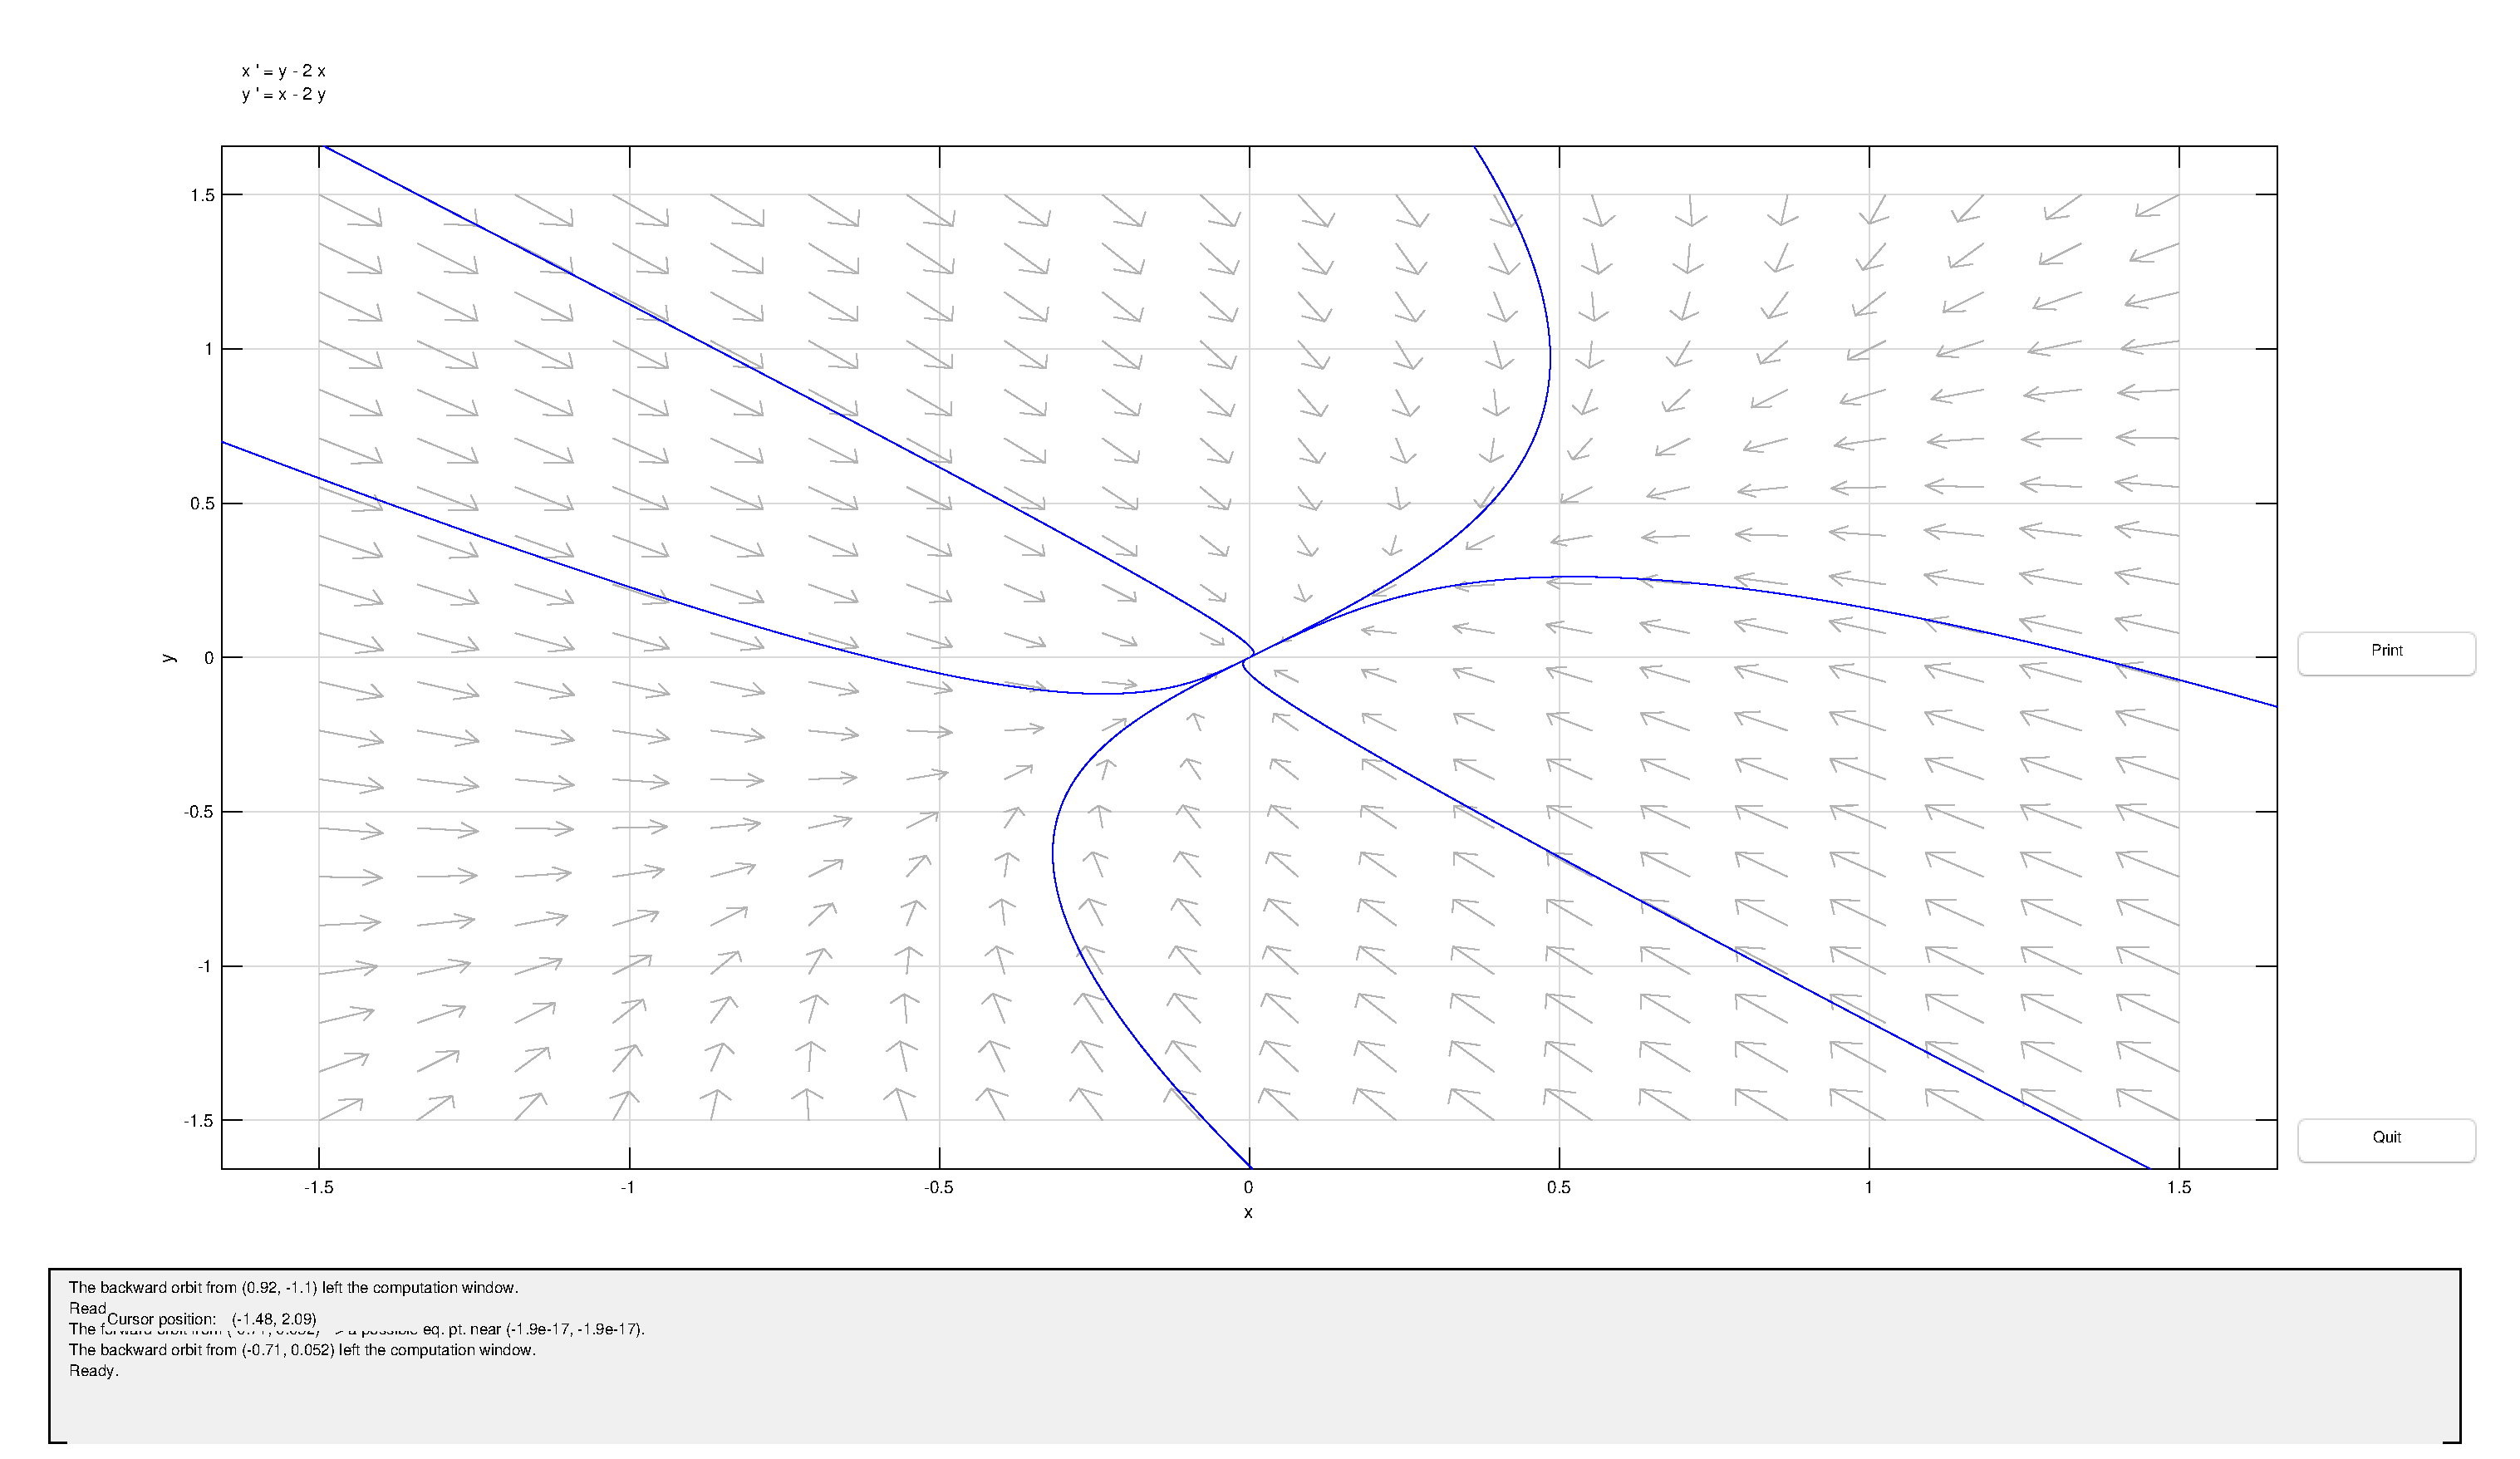
\includegraphics[trim=116 155 125 55,clip,width=\linewidth]{imgs/stable-point}
    \caption{Stable point}%
    \label{fig:stable-point}
  \end{subfigure}
  %
  \begin{subfigure}[b]{0.45\linewidth}
    \centering
    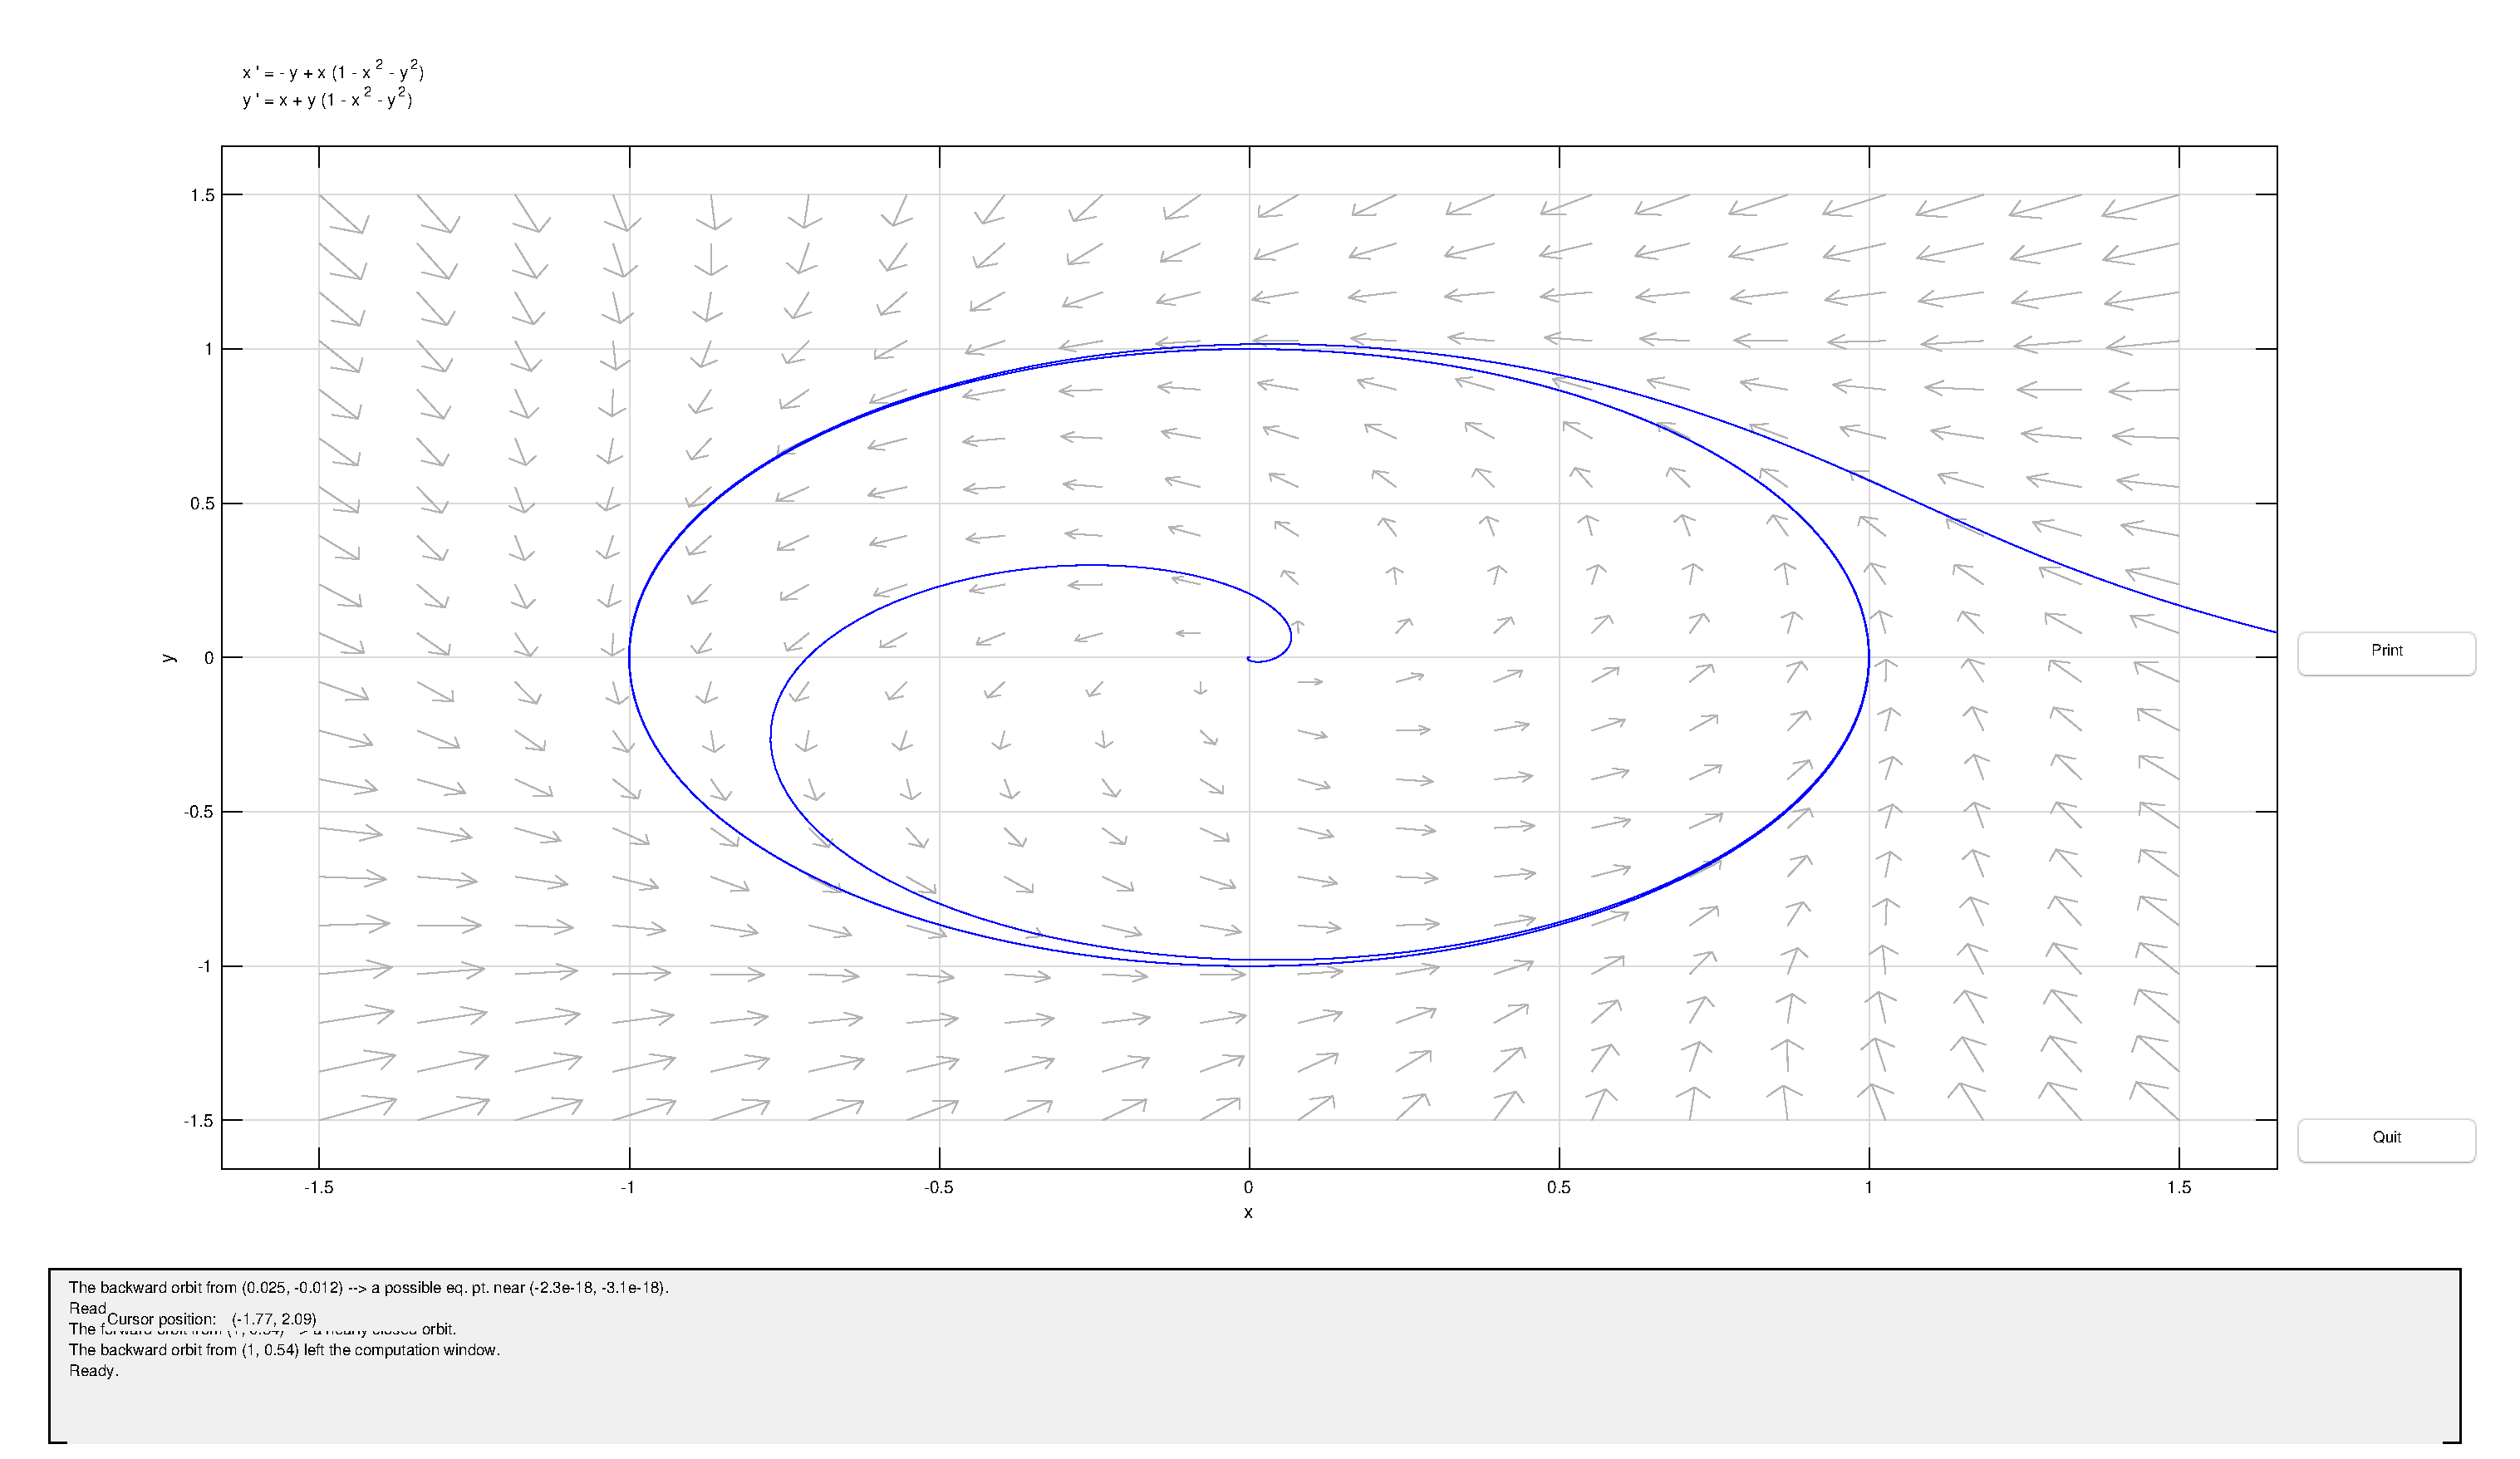
\includegraphics[trim=116 155 125 55,clip,width=\linewidth]{imgs/stable-cycle}
    \caption{Stable cycle}%
    \label{fig:stable-cycle}
  \end{subfigure}
  %
  \begin{subfigure}[b]{0.5\linewidth}
    \centering
    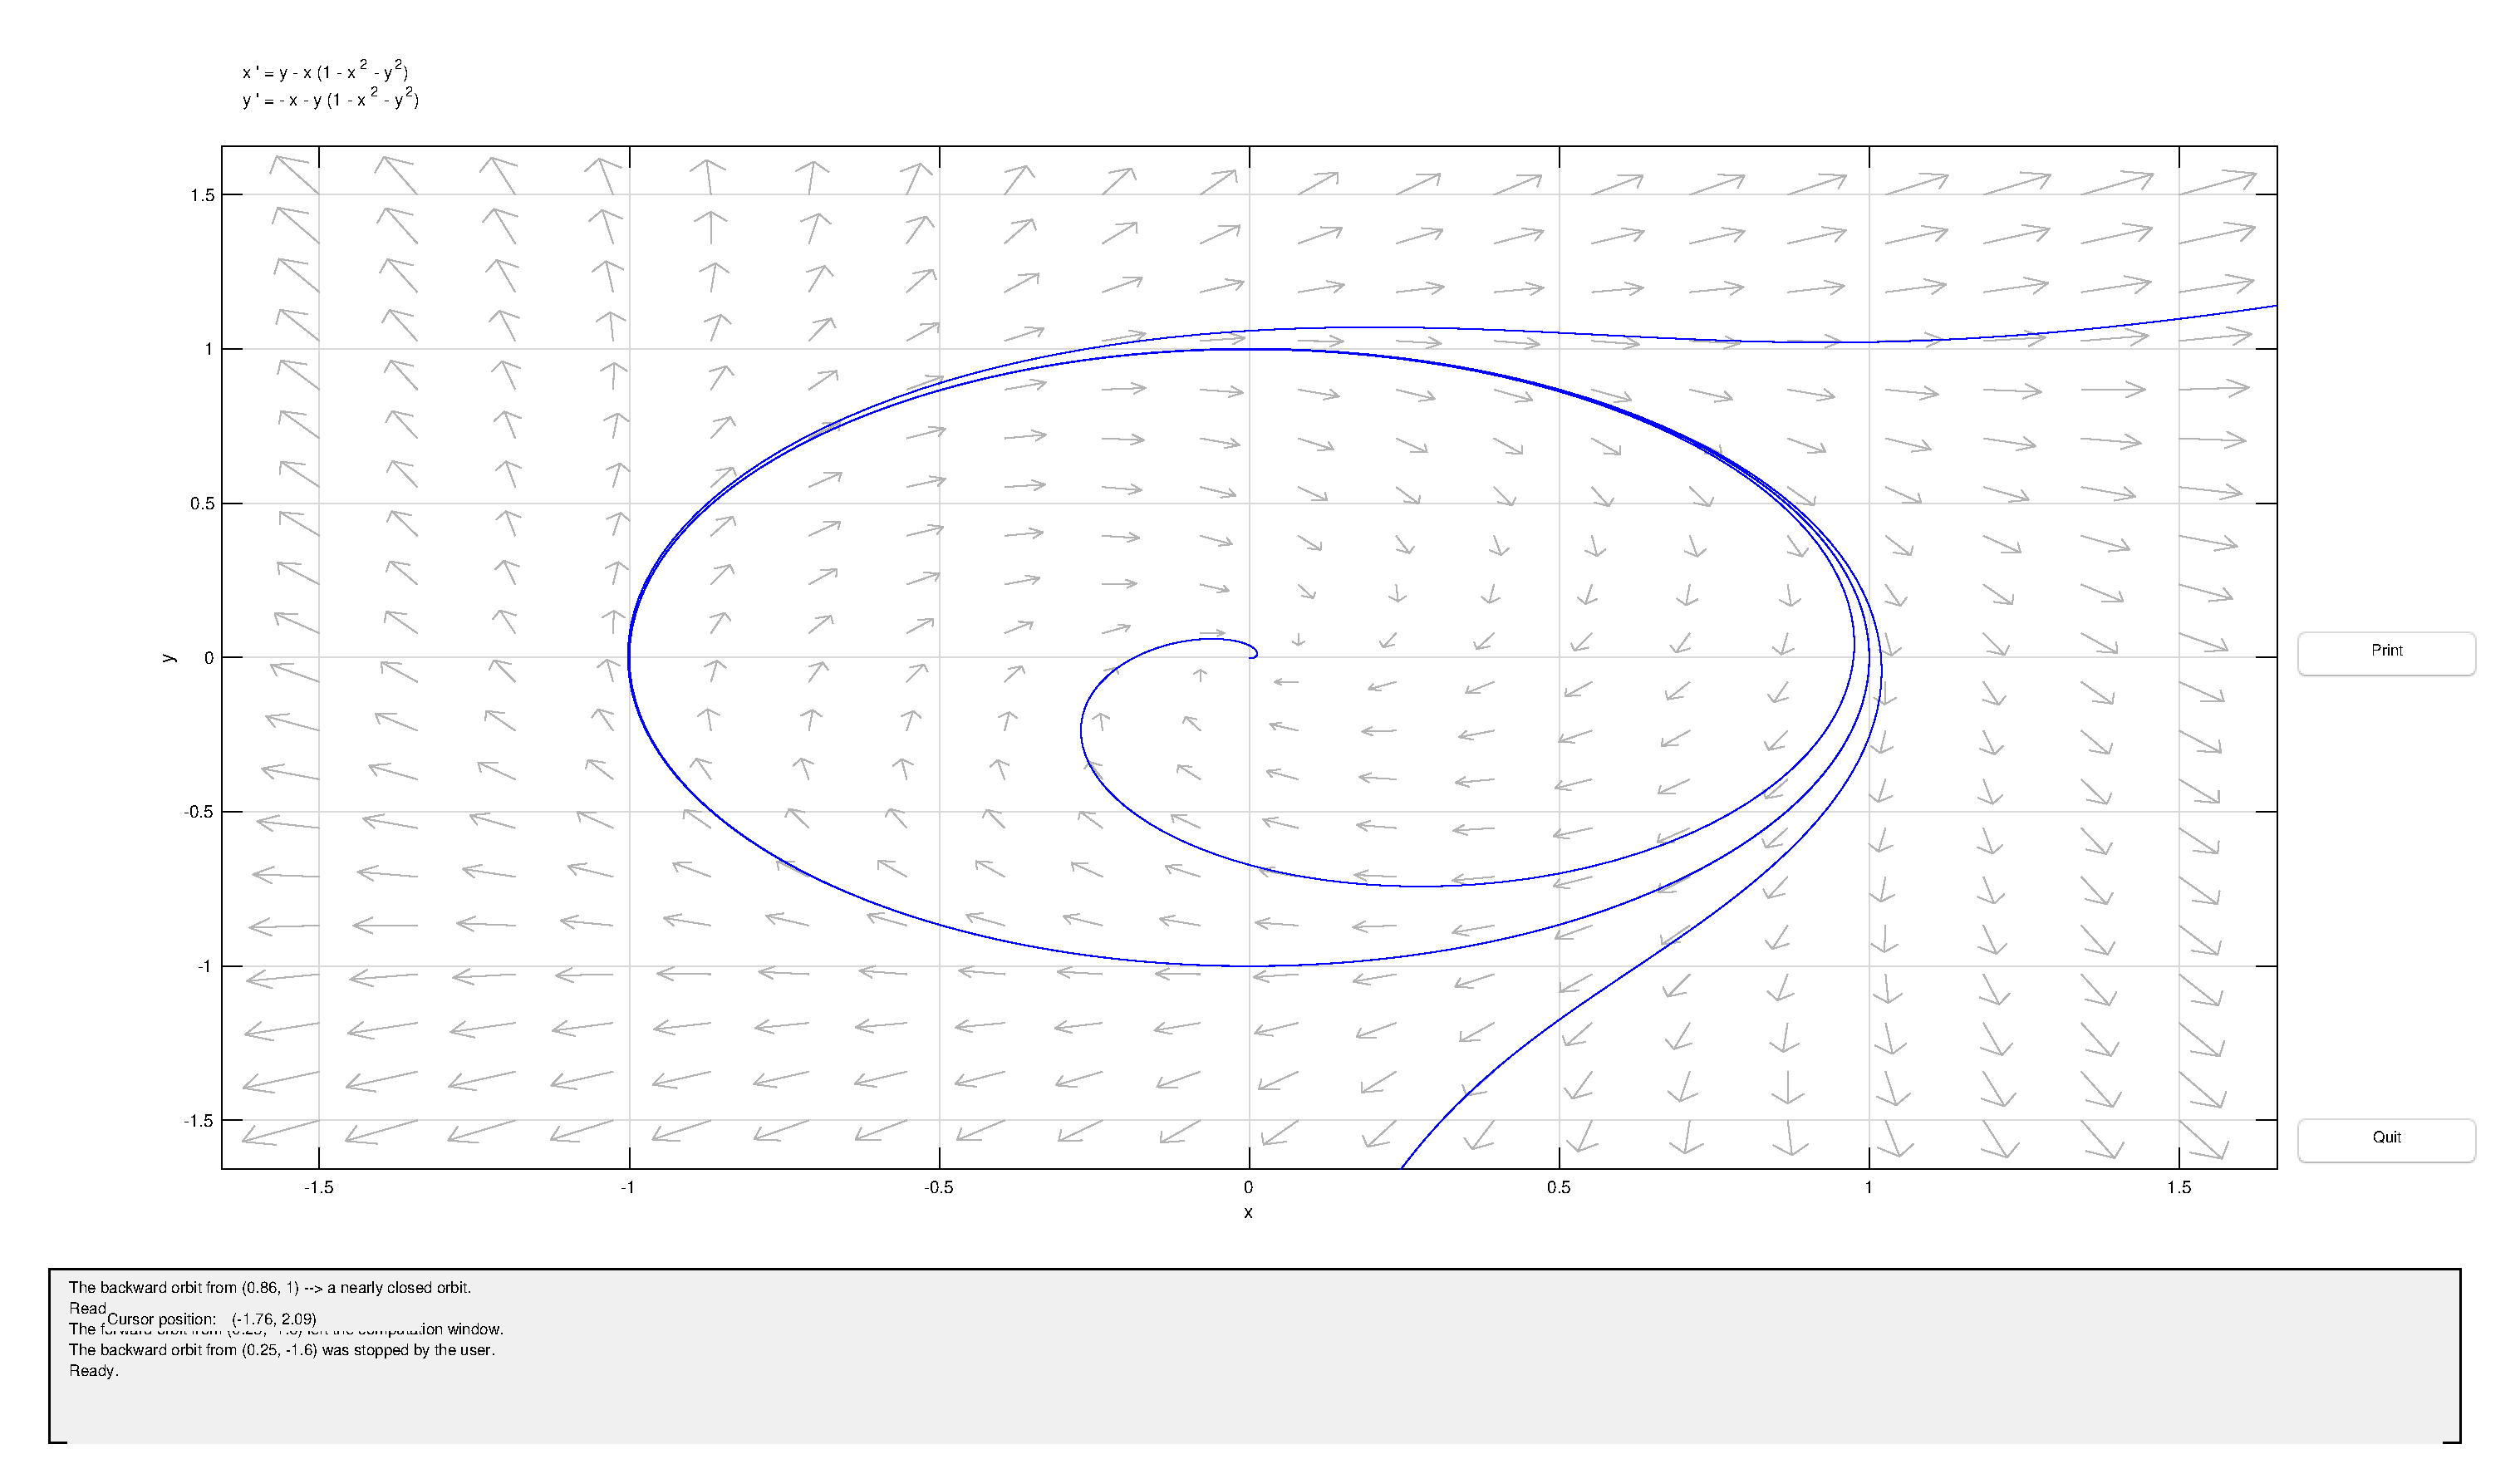
\includegraphics[trim=116 155 125 55,clip,width=\linewidth]{imgs/semi-stable-cycle}
    \caption{Semi-stable cycle}%
    \label{fig:semi-stable-cycle}
  \end{subfigure}
  %
  \caption{Different cycles' gradient maps}%
  \label{fig:poincare-cycles}
\end{figure}

So, by definition, a Region of Attraction is the closed region in the state
plane that guarantees that all initial states inside it will converge to a point
inside of it (usually the origin). This definition does allow stable cycles.

Lyapunov's stability criteria states that for the system \(\dot{x} = f(t, x)\),
if there is a function \(V(x)\) such that

\begin{align}
  V(x)       & = 0 \iff x = 0,                                           \\
  V(x)       & > 0 \iff x \ne 0,                                         \\
  \dot{V}(x) & = \nabla{}V\cdot{}f(x) \le 0 \phantom{0} \forall x \ne 0,
\end{align}

then the system is stable~\parencite{chen:linear,hespanha:linear}. Futhermore,
if \(\dot{V}(x)<0\), the system is asymptotically stable. In this context,
\(V(x)\) is an energy function, but its derivative reminds us of Poincaré's
theorem. In fact, Lyapunov's function can be seen as a more restricted form or
Poincaré's region, which always contains stable points or stable cycles inside
it. If the derivative is strictly negative, the region \(V(x)\) is guarantee to
not contain cycles~\parencite{chen:linear}. Because of this link between the two
theorems, Lyapunov's stability criteria is often used to estimate the region of
attraction.

A common choice of \(V(x)\) is \(V(X)=x^{\top}Px\), which is an ellipsoid. It is
the most used candidate since it is easy to verify its positiviness:
\(V(x)\ge{}0~\forall{}x\) if \(P\) is SDP (semidefinte
positive)~\parencite{bochnak.coste.ea:real}. It is also a simple region to
describe and derive, making it easy to use with LMI tools. Note, however, that
there are infinite possible regions, and \(V(X)=x^{\top}Px\) is most certainly
\textit{not} the largest region, making it a conservative solution.

% !TeX root = document.tex
% !TeX encoding = UTF-8 Unicode

\chapter{Switching Rules}%
\label{chp:switching-rules}

This chapter presents two switching rules: the dwell-time, the most employed and
studied of such techniques in literature, and the proposed rule based on the
region of attraction. Other techniques exist, like using robust control to
design a controller that never allows the system to unstabilize; however, they
are more conservative and not viable in many cases.

\section{Dwell-time}%
\label{sec:dwell-time}

As discussed in Section~\ref{sec:switched-systems}, the act of switching can
cause instability, even if all modes are stable. Although it is possible to
verify if the system is stable under arbitrary switching (and therefore to
design controllers to do so), the procedure is not straight-forward and
challenging to apply to most real-world situations.

There are, however, other ways of verifying and guaranteeing the stability of
systems under switches governed by some rules. The dwell-time is one of such
techniques that restricts the switching signal \(\sigma{}(t)\) to the set
%
\begin{equation}
  \mathcal{D}_{T} := \{\sigma(\cdot):t_{k+1}-t_{k}\ge{}T\},
\end{equation}
%
where \(t_{k}\) and \(t_{k+1}\) are the switching instants, for all
\(k\in{}\mathbb{R}\), which forces the system to remain for \(T\) seconds on a
mode before switching to next one~\parencite{colaneri:dwell}. This is called a
slow switch. The timer is restarted every time the reference changes and
switching is only allowed after \(T\) seconds has passed. For large enough
values of \(T\), this rule guarantees the system's stability.

As the dwell-time certifies stability of the switch, it decouples the switching
logic and the system stability, making it possible to analyse the system
stability for each mode independently. One problem, however, is that computing
the minimum dwell-time is not easy and is the focus of current research. An
easier problem is to find an upper bound for it, which can be done efficiently
using numerical algorithms~\parencite{colaneri:dwell}.

Another technique that uses the concept of dwell-time is the average dwell-time,
where the switching rule \(\sigma\) allows for a fixed number of discontinuities
\(N_{\sigma}(t,\tau)\) for \(t\ge{}\tau{}\ge{}0\) such that the set
\(\mathcal{D}_{T_{D},N_{0}}\) satisfies
%
\begin{equation}
  N_{\sigma}(t,\tau) \le{} N_{0} + \frac{t-\tau}{\tau_{D}},
\end{equation}
%
where \(\tau_{D}\) is the average dwell-time and \(N_{0}\) is the chatter
bound~\parencite{hespanha.morse:stability}. This set is larger than
\(\mathcal{D}_{T}\) and allows for signals with discontinuities separated by at
most \(\tau_{D}\).

To illustrate how the dwell-time works, consider the state-space of a fictional
two-state system shown in Figure~\ref{fig:dt-example}. \(\bullet\) marks the system's
initial state, \(\diamond\) are the waypoints and \(\star\) is the reference. The collored
ellipses are each mode's state's constraints, numbered 1, 2, 3 from left to
right. Since there are three ellipses, we have three modes, meaning three
command governors, controllers and linearized systems. The waypoints are
intermediate references, chosen to allow the system to travel from the current
state (\(\bullet\)) to the reference (\(\star\)) without violating any constraint.

\begin{figure}[ht!]
  \centering
  \begin{tikzpicture}[auto,node distance=3cm,>={Stealth},waypoint/.style={draw,circle,minimum size=1em,inner sep=0pt,outer sep=0pt,thick},state/.style={draw,thick,circle,minimum size=1em,inner sep=0pt,outer sep=0pt},constraint/.style={ellipse,fill opacity=0.7,text opacity=1}]
    \node (x)  [state]                {\(\bullet\)};
    \node (w1) [waypoint,below=of x]  {\(\diamond\)};
    \node (w2) [waypoint,right=of w1] {\(\diamond\)};
    \node (w3) [waypoint,above=of w2] {\(\star\)};

    \begin{scope}[on background layer]
      \node (c1) [constraint,fill=cyan!80,fit=(x) (w1)]    {};
      \node (c2) [constraint,fill=green!80,fit=(w1) (w2)]  {};
      \node (c3) [constraint,fill=orange!80,fit=(w2) (w3)] {};
    \end{scope}

    \draw [->,thick] (x) -- (w1);
    \draw [->,thick] (w1) -- (w2);
    \draw [->,thick] (w2) -- (w3);
  \end{tikzpicture}%
  \caption[Dwell-time illustrative example.]{Dwell-time illustrative example.
    The plane is the phase-plane of a second order system. Each colored region
    represents one mode's contraints, each symbol inside a circle represents a
    point of interest: \(\bullet\) is the initial state, \(\diamond\) are the waypoints and
    \(\star\) the final reference, as set by the operator. The arrows show the path
    the system will take as the supervisor changes the references to the
    waypoints and then to \(\star\).}%
  \label{fig:dt-example}
\end{figure}


Consider that the system is on steady-state at \(\bullet\) when the reference switched
to \(\star\). Since there are three constraints, the supervisor scheme shown in
Figure~\ref{fig:supervisor-schematic} is the same as this examle's one. The
supervisor will receive the new reference \(r(k)\) and, because the system is
currently on mode 1, will set \(r'(k)\) to the first waypoint's coordinates,
since it is not possible to gro from \(\bullet\) to \(\star\) directly without violating
the constraints.

Because a reference change occurred, the supervisor will start a timer, counting
down from the first mode's dwell-time, \(T_{1}\). Even if \(r(k)\) changes
again, \(r'(k)\) will not be changed until this timer expires. This gives the
first mode's controller enough time to converge to the first waypoint,
guaranteeing stability.

Because the waypoint is at mode 1's and mode 2's constraints intersection, the
supervisor is allowed to change the the system to the second mode and change the
reference \(r'(k)\) to the second waypoint's coordinates, as soon as the
dwell-time's timers expire (both changes happen simultaniously). Again, because
the reference changed, a new timer will start, but now counting down from mode
2's dwell-time, \(T_{2}\). The same procedure will be repeated once the system's
state reaches the second waypoint, when \(r'(k)\) will finally be set to
\(r(k)\).

Algorithm~\ref{alg:dwell-time} presents a generalized version of the algorith
described in the given example.

\begin{algorithm}[H]
  \begin{algorithmic}[1]
  \State{}\textbf{Input}: \(\CG{}_i\) \(\leftarrow{}\) current \CG{},~\(\CG{}_j\) \(\leftarrow{}\) target \CG{}.
  \State{}change \(r'(k)\) to next way-point
  \While{dwell-time of \(\CG{}_{i}\) not ellapsed}
    \State{}calculate \(g(k)\)
    \State{}execute controller
  \EndWhile{}
  \State{}change to \(\CG{}_j\)
  \State{}restart algorithm
  \end{algorithmic}
  \caption{dwell-time implementation}%
  \label{alg:dwell-time}
\end{algorithm}

Firstly, \(\CG{}_{i}\) is set to the currently active \CG{} and \(\CG{}_{j}\) to
the next \CG{} in the path (briefly disscussed in
Subsection~\ref{subsec:supervisor}). Then the reference \(r'(k)\) is set to the
next waypoint in the path. The timer is started and the supervisor will wait for
it to ellapse before making any change to the system. While it is not ellapsed,
the active \CG{} and controller will drive the system to the reference
\(r'(k)\). As soon as the time ellapses, the system switches modes, activating
\(\CG{}_{j}\). The procedure is then repeated.

\section{Region of Attraction}%
\label{sec:roa-switching-rule}

The goal of this switching rule is to allow the system to converge faster to the
final reference when going through a path of restricted mode switches. To do so,
it is necessary to:

\begin{enumerate}
  \item guarantee stability after switching modes,
  \item switch modes as soon as possible.
\end{enumerate}

The main contribution of this work is to propose a switching rule based on the
controller's region of attraction yielding a guaranteed stable closed-loop
system. As described in Section~\ref{sec:region-of-attraction}, the controller's
region of attraction is the forward invariant neighbourhood under the flow
generated by a critical point. On a switched system, there is one controller and
linearized system for each mode, therefore there is also one region of
attraction for each mode.

Since the definition of a Region of Attraction undesirably allows the existence
of limit-cycles within the region, we turn to Lyapunov's theorem to further
restrict the region, eliminating them. The set which represents the region of
attraction becomes \textit{contractive}, becoming smaller as the system's state
converges to the critical point. The Lyapunov function is seen as an energy
function, and its value at some point in the state-space is an energy level.
This leads to the so called level sets, which are all points that yield the same
energy level, in Lyapunov's sense.

The level set, denoted \(\mathcal{L}_{V}(P)\), where \(P\) is the matrix used in
the function \(V(x)=x^{\top}Px\), is an estimative of the region of attraction and,
being contractive, implies that, once the system reaches a lower energy level,
in Lyapunov's sense, it can not go to a state with higher energy and can only
stay at the same level if it is zero, which guarantees convergence, as the only
point with zero energy is the origin of the linear system.

The region of attraction is, therefore, a certificate of stability for a system.
However, as stated in Section~\ref{sec:switched-systems}, having stable modes is
not enough to guarantee the stability of the system after switching.
Nonetheless, the following region of attraction based rule guarantees that the
system will remain stable after switching:

\begin{align}
  \sigma_{i} = \begin{cases}
    1 & \textrm{if}~\xi_{i}(k)\in\mathcal{L}_V(P_i) \\
    0 & \textrm{otherwise}
  \end{cases},
\end{align}
%
where \(\xi_{i}(k)\) is the mode's state, and \(\sigma_{i}\) is the switching rule,
meaning that the system can switch to the \(i\)th mode if \(\sigma_{i}=1\). The
switching rule does not force the use of any particular region of attraction
estimation. Any method can be used to estimate the region of attraction, and the
use of Lyapunov's theorem is just an example.

Let us discuss the stability of the system when this rule is used. Suppose a
system with two modes is currently in mode 1, and the supervisor has deemed that
it needs to go mode 2. The switch will only occur when the system's state is
inside the second mode's controller's region of attraction. Because it is inside
the region of attraction, it guarantees that it will converge, and therefore the
switch is stable.

Consider the same scenario, however the system has 10 modes and the switch from
mode 1 to mode 2 follows the path \(1 \rightarrow 3 \rightarrow 8 \rightarrow 2\), meaning that, to go from
\(1\) to \(2\), it first needs to switch to \(3\), then to \(8\) and only then
to \(2\). The worst-case would be if the system is in the middle of the
intersection of all regions of attraction. In this case, the system will
instantly switch modes, going from \(1\) to \(2\) in \(3\) sample times, in the
case of a discrete system. However, since the switch can only happen when the
state is inside the next mode's controller's region of attraction, it will
simply cause the previous scenario to be applied recursivelly, and the system
will remain stable after it reaches the last mode.

In another scenario, the software generating the references for the supervisor
(i.e. generating \(r(k)\)) might malfunction or have a badly defined rule that
will make the reference jump between many values, making the system try to
switch modes seemly randomly. In this case the system will do the switches as
long as it is allowed, but the state will always be inside some controller's
region of attraction. It will then either never converge nor diverge (because of
the ever-changing reference) or enter a state that is only inside one mode's
controller's region of attraction, at which point it will not switch modes
anymore.

The illustrative scenarios show that the state will always be inside some
controller's region of attraction, and therefore it is not possible for the
system to diverge. It can oscilate due to varying references, but that is a case
of malfunction or badly desined referencing system, not normal operation.
Furthermore, when used in conjunction with Command Governors, the reference is
always guaranteed to be inside the region of attraction (since the constraint
region is completely contained inside it), even if the supervisor's reference is
not, eliminating the possible scenario where the system diverges because the
reference is outside the region of attraction, dragging the system out of it.

To illustrate, we will use the same example of Section~\ref{sec:dwell-time}, but
this time applying the region of attraction based rule. A difference, seen in
Figure~\ref{fig:roa-example}, is the presence of the dashed circles,
representing each controller's region of attraction. When the reference
\(r'(k)\) changes to the first waypoint's coordinates, the supervisor will start
checking whether the system's state is inside the region of attraction of the
next mode's controller and, when it enters this region, the controller and
linearized model will be changed to those of the system's mode 2, but the
constraints will still be those of mode 1. We call this a hybrid switch. In
Figure~\ref{fig:roa-example}, the dashed arrows represent a path followed while
in a hybrid mode.

\begin{figure}[ht!]
  \centering
  \captionsetup{justification=centering}
  \begin{tikzpicture}[auto,node distance=3cm,>={Stealth},waypoint/.style={draw,circle,minimum size=1em,inner sep=0pt,outer sep=0pt,thick},state/.style={draw,thick,circle,minimum size=1em,inner sep=0pt,outer sep=0pt},constraint/.style={ellipse,fill opacity=0.7,text opacity=1}]
    \node (x)  [state]                {\(\bullet\)};
    \node (w1) [waypoint,below=of x]  {\(\diamond\)};
    \node (w2) [waypoint,right=of w1] {\(\diamond\)};
    \node (w3) [waypoint,above=of w2] {\(\star\)};

    \begin{pgfonlayer}{background}
      \node (c1) [name path=c1,constraint,fill=cyan!80,fit=(x) (w1)]    {};
      \node (c2) [name path=c2,constraint,fill=green!80,fit=(w1) (w2)]  {};
      \node (c3) [name path=c3,constraint,fill=orange!80,fit=(w2) (w3)] {};
    \end{pgfonlayer}

    \node (roa1) [circle,very thick,draw=cyan!80,dashed,fit=(c1)]   {};
    \node (roa2) [circle,very thick,draw=green!80,dashed,fit=(c2)]  {};
    \node (roa3) [circle,very thick,draw=orange!80,dashed,fit=(c3)] {};

    \coordinate (i11) at (intersection of w1--x and roa2);
    \path[name path=xw1] (x)--(w1);
    \path[name intersections={of=xw1 and c2,by=i12}];

    \coordinate (i21) at (intersection of w2--w1 and roa3);
    \path[name path=xw2] (w1)--(w2);
    \path[name intersections={of=xw2 and c3,by=i22}];

    \draw [->,thick]        (x) -- (i11);
    \draw [->,thick,dashed] (i11) -- (i12);
    \draw [->,thick]        (i12) -- (i21);
    \draw [->,thick,dashed] (i21) -- (i22);
    \draw [->,thick]        (i22) -- (w3);
  \end{tikzpicture}%
  \caption{Region of attraction illustrative example}%
  \label{fig:roa-example}
\end{figure}


The advantage of the hybrid switch is the possibility to speedup convergence. It
is not required, but if the second controller is known to have a desired better
performance index, it can be allowed. If it is known that it performs worse,
this rule can be ignored. Here we assume that switching earlier always results
in faster convergence to highlight in the figure when those changes would occur.

While in this hybrid mode, the system continues to converge to the waypoint. The
supervisor checks at each instant whether the system's state is inside the
current and next mode's constraint's intersection. Upon entering the
intersection, a full mode switch is performed, activating mode 2's command
governor and constraints. The supervisor sets the reference \(r'(k)\) to the
next waypoint in path, in this case the second one, and system is free to
converge to it.

The same procedure will be repeated, with a hybrid switch occurring when the
system's states enters the third mode's controller's region of attraction and
another full switch when it enters modes 2 and 3's constraints intersection.

With this switching rule, there is no wait: the system will change mode as soon
as possible, yielding faster overall convergence. The hybrid switching is an
addition that may increase the performance of the system at the cost of
computation resources, but is not necessary and can be safelly ignored.
Algorithm~\ref{alg:roa-rule} shows the proposed rule in both its forms, assuming
the use of a Command Governor, which is always recommended for this rule as it
helps to guarantee stability.

\begin{algorithm}[H]
  \begin{algorithmic}[1]
    \State{}\textbf{Input}: \(\CG{}_i\leftarrow{}\) current \CG{},~\(\CG{}_j\leftarrow{}\) target \CG{}.
    \State{}\textbf{let} \(P_j\) be the \(P\) matrix of \(\CG{}_j\)'s Lyapunov function.
    \If{should switch controllers earlier}
      \While{\(\xi(k)\not\in\mathcal{L}_V(P_j)\)}
        \State{}calculate \(g(k)\)
        \State{}execute controller
      \EndWhile{}
      \State{}change current controller and model to \(\CG{}_j\)'s ones
      \State{}reset integrators
    \EndIf{}
    \While{\(x(k)\not\in\mathcal{X}_i\cap\mathcal{X}_j\) or \(\hat{\xi}(k)\not\in\mathcal{L}_V(P_j)\)}
      \State{}calculate \(g(k)\)
      \State{}execute controller
    \EndWhile{}
    \State{}change to \(\CG{}_j\)
    \State{}reset integrators if not already done
    \State{}change \(r(k)\) to next way-point
    \State{}restart algorithm
  \end{algorithmic}
  \caption{Switching rule based on region of attraction}%
  \label{alg:roa-rule}
\end{algorithm}

\(\CG{}_{i}\) is the currently active \CG{} and \(\CG{}_{2}\) is the next \CG{}
in the path. \(P_{j}\) is next \CG{}'s Lyapunov function's \(P\) matrix.
\texttt{should switch controllers earlier} tests whether a hybrid from
\(\CG{}_{i}\) to \(\CG{}_{j}\) is allowed. If it is, the supervisor checks if
the system's state is inside next mode's controller's region of attraction.
While it is not, the current controller is executed, alogside its \CG{} unit.
Once the system enters the next mode's controller's region of attraction, the
controller and internal linearized model are switched, taking the necessary
measures to guarantee continuity of signals, specially control signal, such as
resetting integrators. This controller is executed until the system's state
enters the current and next mode's constraint's intersection, when the full mode
switch occurs. The reference \(r'(k)\) is set to the next waypoint's coordinates
and the algorithm is restarted.

\section{Practical Implementation Aspects}%
\label{sec:practival-implementation-aspects}

When implementing the techniques described in this thesis, some details need
attention. For example, it is easy to say
\enquote{\(\mathrm{minimize}~f(x)~|~x\in\mathcal{X}\)}, however it is not so
simple (and sometimes even impossible) to implement the set membership check
\(x\in\mathcal{X}\). Describing the set and finding a way to test membership
numerically can be challenging. That is one reason why we choose convex sets: we
know how to implement membership tests and use it in common optimization
frameworks.

This chapter will discuss how to represent the constraints and region of
attraction and provide some insight into how to implement the models of the
command governor with a supervisor structure, and the problems faced when
estimating the region of attraction.

\subsection{Polytope representations}%
\label{subsec:polytope-representation}

A convex polytope can approximate any convex region. A convex polytope is a
compact convex set with a finite number of extreme points such that, for any two
distinct points \((a,b)\) belonging to the region, a closed segment with
endpoints \((a,b)\) is entirely contained within the
region~\parencite{grünbaum:convex}. In other words, it is a convex hull of a
finite number of points, called vertices. This representation is called the
\enquote{V-representation} in \(\mathcal{R}^{2}\) and is not useful to test
membership. However, it is straightforward to sample points from the desired
region's border to create a V-representation of a polytope approximating it. It
is also useful for plotting. The Figure~\ref{fig:v-rep-example} illustrates a
region in its V-representation, where the red dots are the vertices, and all
blue dots are inside the region. The set of vertices is
\resizebox{\linewidth}{!}{%
  \(\{(0.02,0.71),(0.31,0.02),(0.82,0.04),(0.87,0.13),(0.99,0.88),(0.60,0.98),(0.38,0.97),(0.04,0.88),(0.02,0.82)\}\)}.

\begin{figure}[!htb]
  \centering
  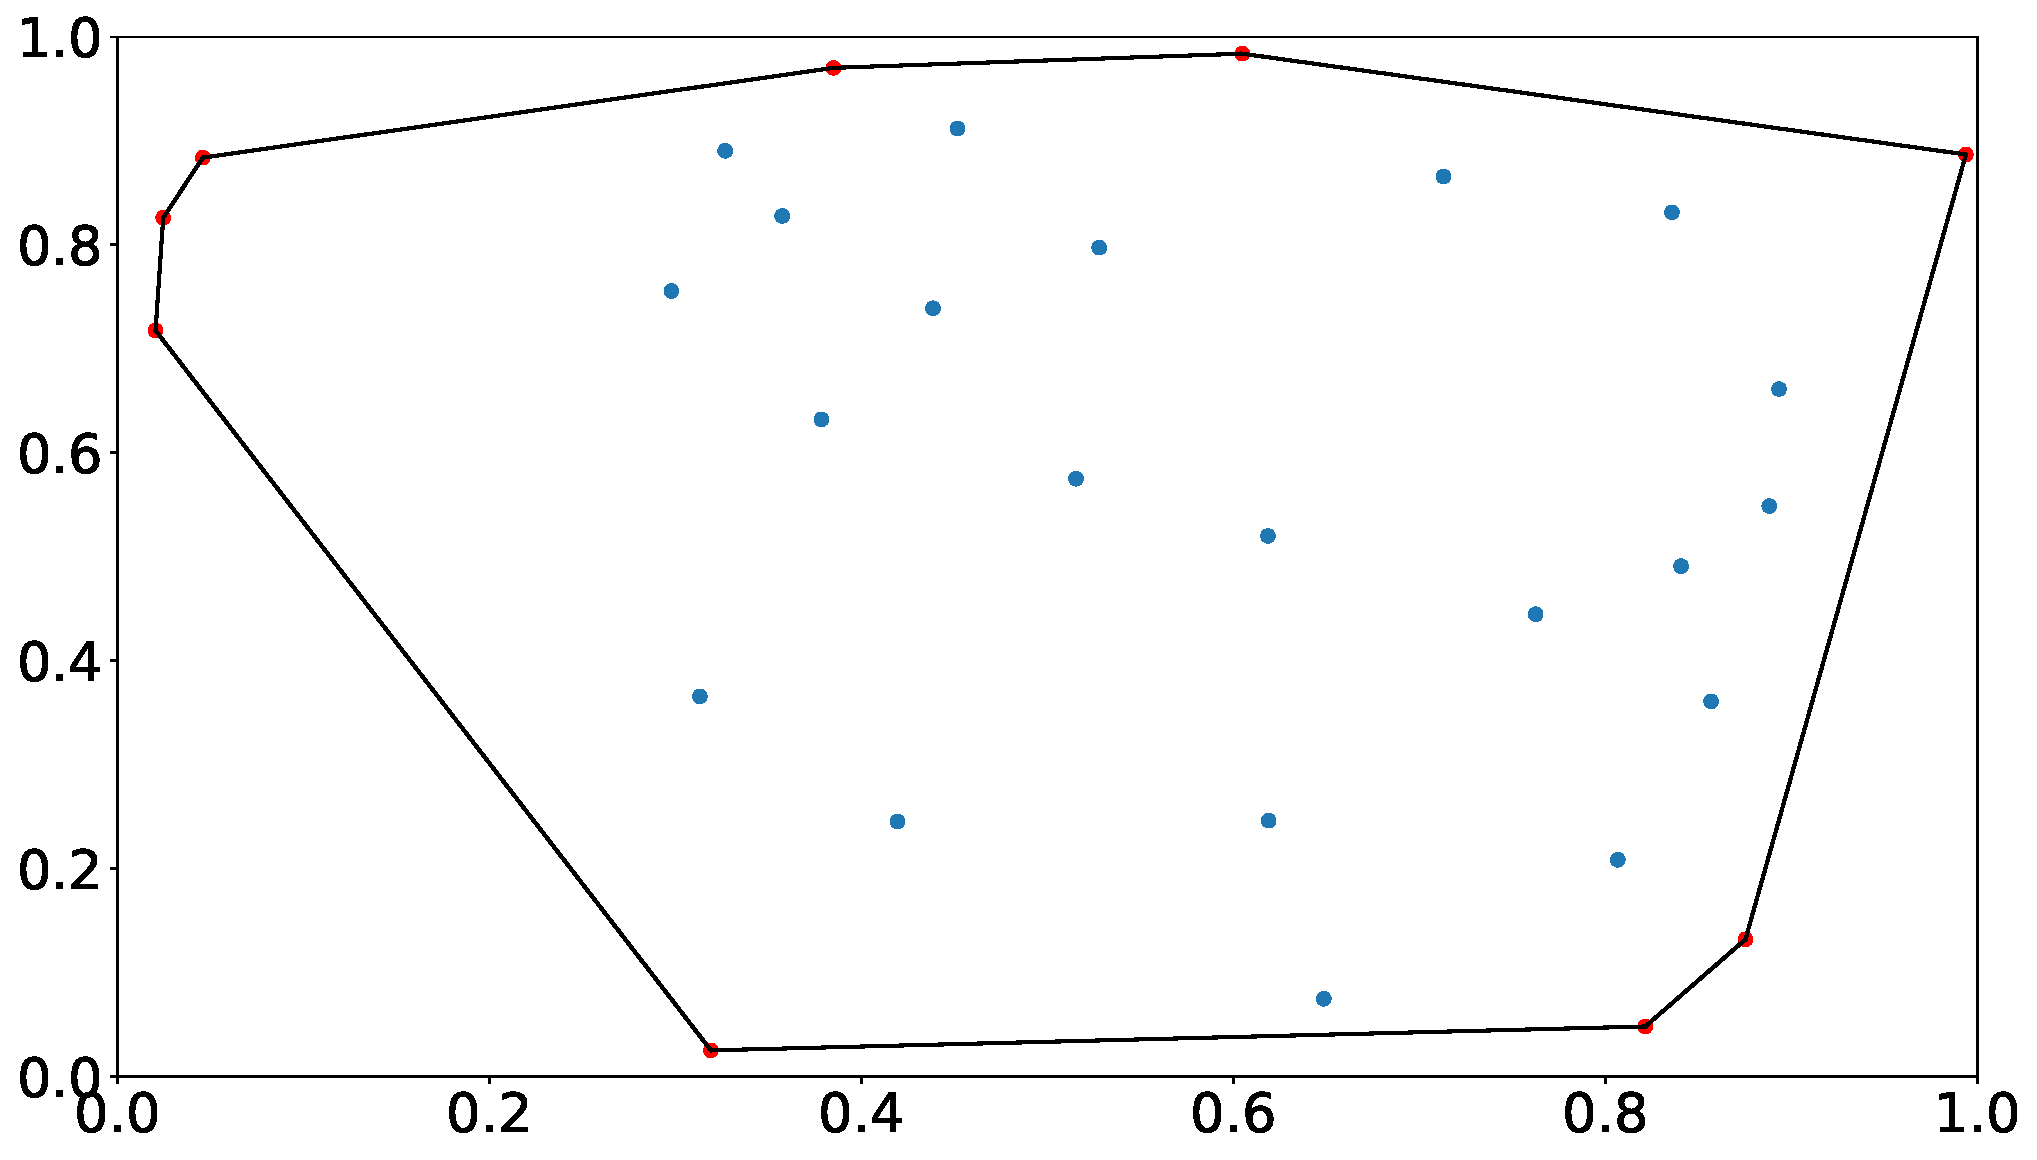
\includegraphics[width=\linewidth]{imgs/v-rep}
  \caption{Visualization of the V-representation of a set}%
  \label{fig:v-rep-example}
\end{figure}

A more useful representation of such regions is the \enquote{H-representation}.
In such a representation, the intersection of a finite number of half-spaces
describes the region. A half-space is one of the two parts in which a
hyper-plane divides an affine space. Since half-spaces are linear inequalities,
the H-representation becomes the matrix inequality
%
\begin{equation}
  Ax\leq{}b,
\end{equation}
%
where \(A\) is a matrix of coefficients, \(x\) is a point in space and \(b\) is
a vector of real numbers. The number of rows in \(A\) and \(b\) is the same as
the number of half-spaces defining the region. All points satisfying the
inequality are in the region's interior, making it easy to test set membership.
Figure~\ref{fig:h-rep-example} shows the half-spaces that compose the
H-representation of the same convex polytope presented in
Figure~\ref{fig:v-rep-example}. Equation~\ref{eq:h-rep-example} shows the
inequation that describes the region. The selected side is not shown for each
half-space but is the one in which intersections with the other selected halves
make the convex region in the middle.

\begin{equation}
  \label{eq:h-rep-example}
  \begin{bmatrix}
    -0.91 & -0.39 \\
    0.04  & -0.99 \\
    0.98  & -0.15 \\
    0.84  & -0.54 \\
    -0.24 & 0.96  \\
    0.24  & 0.97  \\
    -0.06 & 0.99  \\
    -0.99 & 0.03  \\
    -0.93 & 0.34
  \end{bmatrix}x \leq
  \begin{bmatrix}
    -0.30 \\
    -0.01 \\
    0.84  \\
    0.66  \\
    0.84  \\
    1.10  \\
    0.94  \\
    0.00  \\
    0.26
  \end{bmatrix}
\end{equation}

\begin{figure}[!htb]
  \centering
  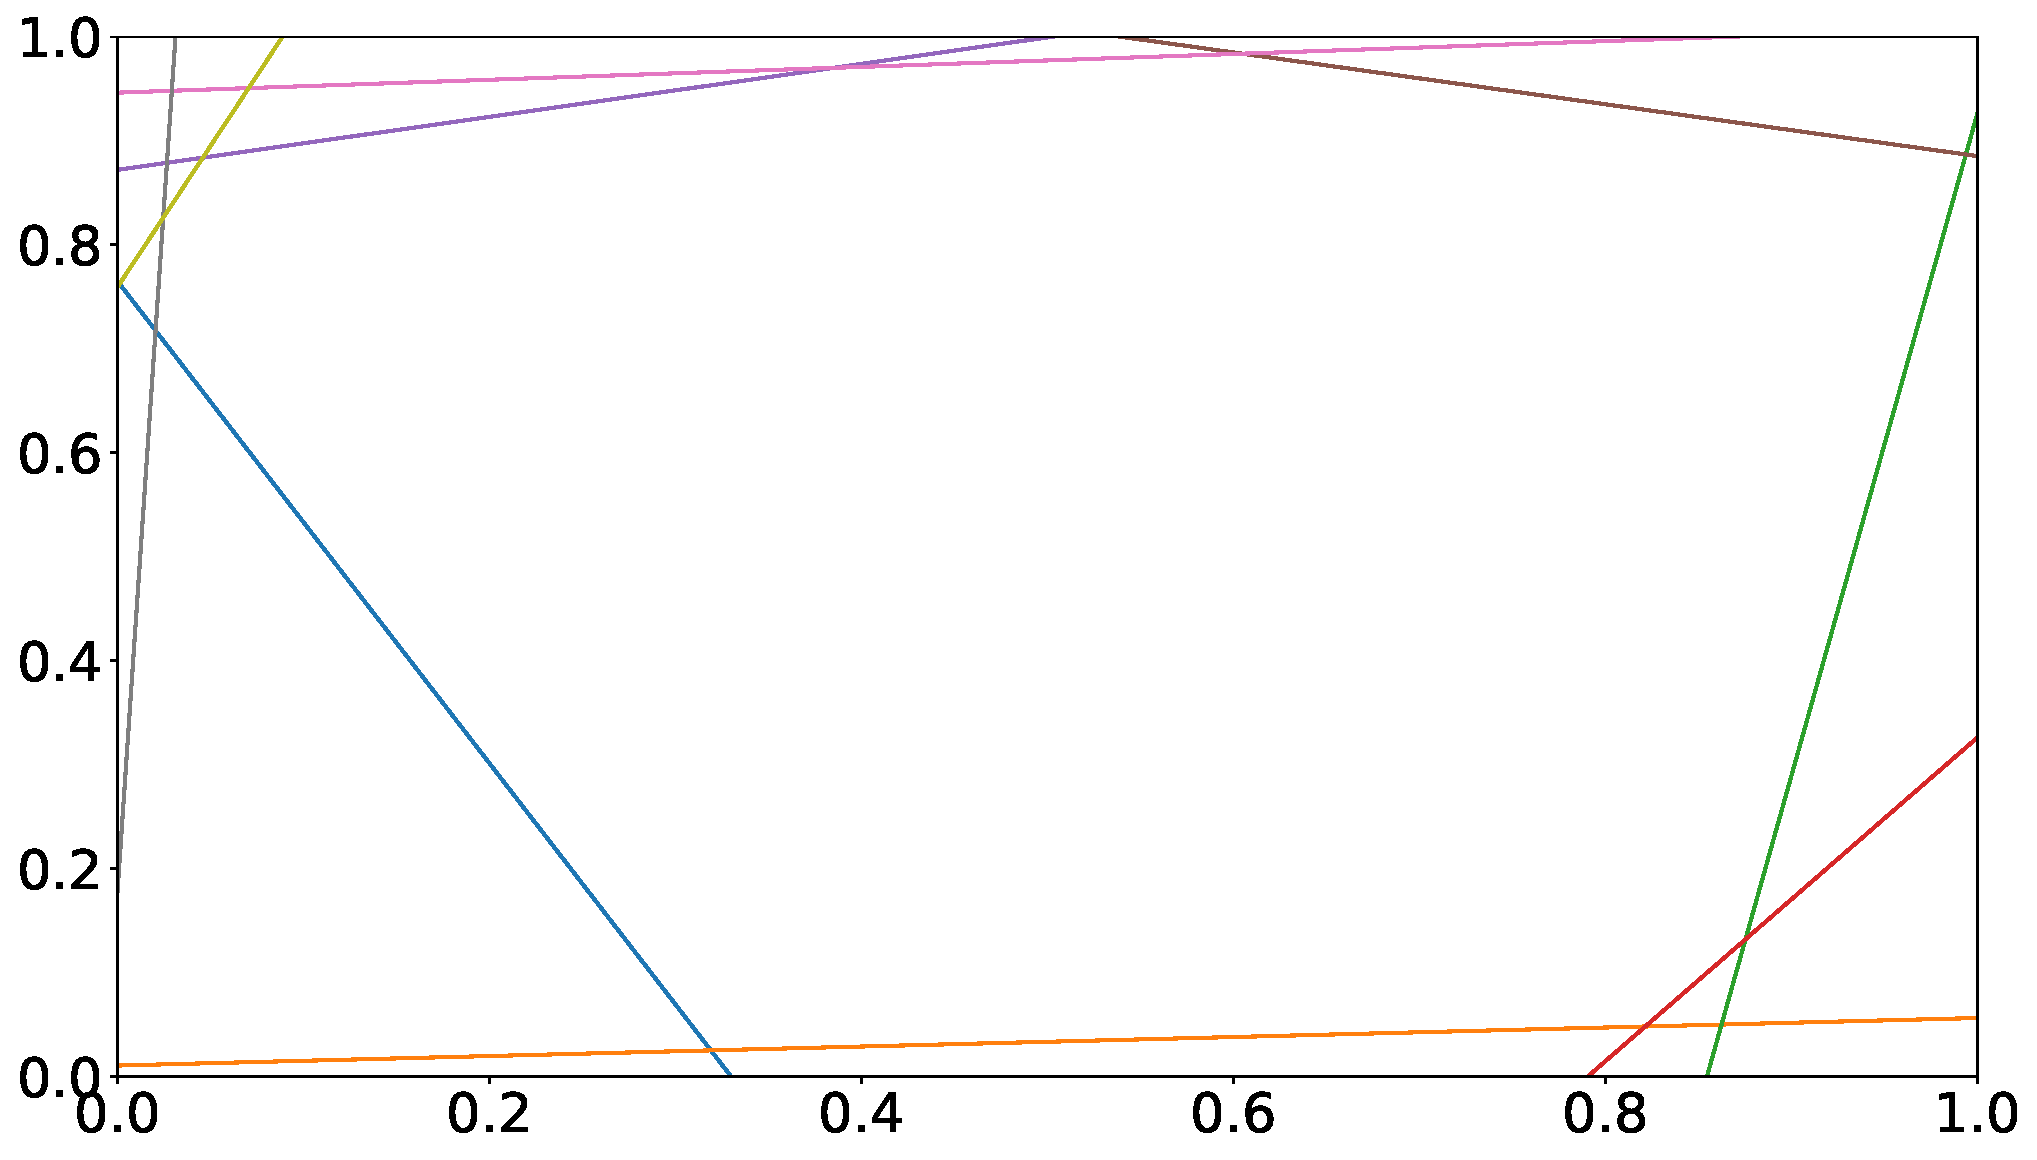
\includegraphics[width=\linewidth]{imgs/h-rep}
  \caption{Visualization of the H-representation of a set}%
  \label{fig:h-rep-example}
\end{figure}

Given that the V-representation is easier to obtain from generic shapes, but the
H-representation is more useful when verifying set membership, it is essential
to have a way to switch between them. Unfortunately, this is not
straightforward, but some algorithms allow us to enumerate the facets given the
vertices. Some problems of such algorithms are the time needed to find the
facets of many vertices and how to find facets in higher-order spaces. However,
good algorithms can be used for the conversion, especially if the computation
will be offline
\parencite{avis.bremner.ea:how,graham.frances-yao:finding,lee:on,mccallum.avis:linear}.

Particular regions can be easily described in a way that is easy to include in
optimization problems. The ellipsoid is one such region, as it is described as
\(x^{\top}Px\leq{}1\) so that any point \(x\) that satisfies the inequality is inside
the region. Any region described by polynomials can be expressed in a matrix
form and can quickly test membership. Such regions should use their inequation
directly instead of a polytope approximation. We do that to the Region of
Attraction, and it is how we implemented the check to verify if the state is
inside it.

\subsection{Internal Models}%
\label{subsec:internal-models}

To switch modes and controllers of a system the way we propose, one must pay
attention to the controller's internal states and the control signal's
continuity. Also, since every \CG{} unit has its controller and model, the
destination \CG{} must be updated to a valid state before switching. There are
many ways to do so, and we will present some.

One way is to run all \CG{}s in parallel. The optimization problem of the
inactive units does not need to run with complete constraints. It can be relaxed
only to contain the region constraint on the virtual reference; also, the
observer can be ignored. It is necessary to find the virtual reference, which
will be close to the constraint region's border, which is closest to the real
system's state. Notice that, in this case, we are not looking for a virtual
reference closest to the real reference but to the real system's state. By doing
so, the internal model's and the controller's states will always be valid.

However, this approach can be resource-intensive, as it still computes the
optimization problem at every sample. It is also possible to run the observer
and update the internal model's states without checking for constraint
violations, but this does not solve the controller's state problem. Another
technique needs to be combined to find them.

Another way of guaranteeing valid states is to compute the states before
changing mode. Two ways of computing the states are: by inverting the system and
controller equations and by simulation. The first approach has a very low
computational resource impact but may not be possible or yield not ideal values.
For systems with integrators, for example, there will be infinitely many
results. Another problem is that even though the system has only one
steady-state solution, it can have many transient ones.

The simulation becomes interesting, even though it is more computationally
intensive, as it can calculate a state that better matches the current
transitory characteristics of the real system. It can also find the model's and
controller's states at once, guaranteeing that there is no mismatch. To use the
simulation approach, execute the simulation right before changing modes, using
the internal controller and model, and setting the reference to the real
system's current state. This yields a valid steady-state model's and
controller's state. However, this technique does not guarantee control signal
continuity (which might even be impossible on some systems) without adjustments.

\subsection{Region of Attraction Estimation}%
\label{subsec:roa-estimation}

The Lyapunov approach presented in Section~\ref{subsec:region-of-attraction} can
easily estimate the region of attraction. The presented approach makes use of a
quadratic Lyapunov candidate, but it is not necessary, as it is possible to find
functions of any form. The function should easily to check if a point belongs to
the region, as it will be done frequently. Quadratic forms, such as the simple
one presented or those generated by Sum Of Squares techniques, are recommended
since they easily and computationally inexpensively check set membership.

The region of attraction needs to be larger than the constraints region and
needs to intersect all mode's regions of attraction to and from which it can
switch. Because of this, it is necessary to guarantee the intersection. However,
LMIs usually try to optimize the size of the region of attraction by making it
as big as possible or as small as possible. Since the exponential stability
tries to minimize the size of the region of attraction, we need a way to ensure
a minimum region size.

Consider the region of attraction described by
%
\begin{equation}
  x^{\top}Px \le{} 1,
\end{equation}
%
where \(x\) is the point that should be inside the region of attraction. Note
that, numerically, a number smaller than \(1\) may be necessary to make the
problem feasible.

If the LMI is written in terms os \(P\), it can be used directly to force the
region to be big enough to contain the point \(x\). If the LMI is written in
terms of \(P^{-1}\), simply applying Schur's complement yields a valid LMI:
%
\begin{equation}
  \label{eq:lmi-point-inside-roa}
  \begin{bmatrix}
    P^{-1}   & x \\
    x^{\top} & 1
  \end{bmatrix} \succ \mathbf{0},
\end{equation}

You need to add one of such LMIs to your optimization problem for each mode that
is allowed to switch from or to the current mode. The point \(x\) does not need
to be the same for two modes that intersect, as placing the points some distance
apart creates a larger region of intersection, which gives a margin for errors.

To illustrate the choice of \(x\), consider the switched system composed of
three modes shown in Figure~\ref{fig:choice-x-roa-diff}. The stars represent
each mode's linearization point, the filled ellipses its constraints regions,
the unfilled circles the regions of attractions and the black dots the points
used in the LMIs to ensure the RoA's size. Note the intersection region formed
in the middle, displayed in yellow.

Now compare it with the same system, but only one point used for all systems,
depicted in Figure~\ref{fig:choice-x-roa-same}. See how smaller is the
intersection of regions of attraction and constraints (in yellow). The proposed
technique will be much more efficient in the first case, since it will result in
an earlier switch.

\begin{figure}[!htb]
  \centering
  \begin{subfigure}[b]{.45\linewidth}
    \centering
    \includesvg[width=\linewidth]{imgs/roa-choice-of-x-diff.svg}
    \caption{Choosing different \(x\) for each RoA}%
    \label{fig:choice-x-roa-diff}
  \end{subfigure}
  %
  \begin{subfigure}[b]{.45\linewidth}
    \centering
    \includesvg[width=\linewidth]{imgs/roa-choice-of-x-same.svg}
    \caption{Choosing the same \(x\) for all RoA}%
    \label{fig:choice-x-roa-same}
  \end{subfigure}
  \caption{Different RoA's intesections}%
  \label{fig:choices-of-x}
\end{figure}

% !TeX root = document.tex
% !TeX encoding = UTF-8 Unicode

\chapter{Results}%
\label{chp:results}

This chapter presents both simulations and experimental results that show the
technique working and compares it with dwell-time implementations.

For all simulations and experiments in this chapter, the controller is designed
to ensure null steady-state error for piecewise constant references at each mode
\(i\), and thus the integral action is applied over the tracking
error~\parencite{lopes.leite.ea:anti-windup}
%
\begin{equation}
  \label{eq:r-y-error}
  e(k) = r(k)-y(k),
\end{equation}
%
where \(r(k)\) is the desired output of the system. The proportional action
comes from the system's state deviation with respect to the equilibrium point.
Figure~\ref{fig:pi-controller-diagram} depicts the topology of the considered
controller.

\begin{figure}[!htb]
  \centering
  \resizebox{0.98\linewidth}{!}{\setlength{\unitlength}{4144sp}%
%
\begingroup\makeatletter\ifx\SetFigFont\undefined%
\gdef\SetFigFont#1#2#3#4#5{%
  \reset@font\fontsize{#1}{#2pt}%
  \fontfamily{#3}\fontseries{#4}\fontshape{#5}%
  \selectfont}%
\fi\endgroup%
\begin{picture}(10169,2767)(1914,-4943)
\thinlines
{\color[rgb]{0,0,0}\put(8866,-3301){\vector( 0, 1){630}}
}%
{\color[rgb]{0,0,0}\multiput(8551,-3211)(9.00000,0.00000){66}{\makebox(1.5875,11.1125){\tiny.}}
}%
{\color[rgb]{0,0,0}\multiput(9091,-2806)(-9.00000,0.00000){66}{\makebox(1.5875,11.1125){\tiny.}}
}%
{\color[rgb]{0,0,0}\put(8236,-2986){\vector( 1, 0){1260}}
}%
{\color[rgb]{0,0,0}\put(9377,-2809){\line(-1, 0){270}}
\put(9107,-2809){\line(-3,-2){591.923}}
\put(8522,-3214){\line(-1, 0){270}}
}%
\thicklines
{\color[rgb]{0,0,0}\put(8191,-3346){\framebox(1440,720){}}
}%
{\color[rgb]{0,0,0}\put(10576,-2356){\line(-1, 0){  2}}
\multiput(10565,-2358)(-10.00000,-2.00000){2}{\makebox(6.3500,9.5250){\small.}}
\multiput(10555,-2360)(-12.94120,-3.23530){2}{\makebox(6.3500,9.5250){\small.}}
\multiput(10542,-2363)(-8.00000,-2.00000){3}{\makebox(6.3500,9.5250){\small.}}
\multiput(10526,-2367)(-9.03845,-1.80769){3}{\makebox(6.3500,9.5250){\small.}}
\multiput(10508,-2371)(-10.94120,-2.73530){3}{\makebox(6.3500,9.5250){\small.}}
\multiput(10486,-2376)(-11.52940,-2.88235){3}{\makebox(6.3500,9.5250){\small.}}
\multiput(10463,-2382)(-8.31373,-2.07843){4}{\makebox(6.3500,9.5250){\small.}}
\multiput(10438,-2388)(-8.60000,-2.86667){4}{\makebox(6.3500,9.5250){\small.}}
\multiput(10412,-2396)(-8.60000,-2.86667){4}{\makebox(6.3500,9.5250){\small.}}
\multiput(10386,-2404)(-9.00000,-3.00000){4}{\makebox(6.3500,9.5250){\small.}}
\multiput(10359,-2413)(-8.90803,-3.56321){4}{\makebox(6.3500,9.5250){\small.}}
\multiput(10332,-2423)(-9.31033,-3.72413){4}{\makebox(6.3500,9.5250){\small.}}
\multiput(10304,-2434)(-9.71263,-3.88505){4}{\makebox(6.3500,9.5250){\small.}}
\multiput(10275,-2446)(-7.20000,-3.60000){5}{\makebox(6.3500,9.5250){\small.}}
\multiput(10246,-2460)(-7.60000,-3.80000){5}{\makebox(6.3500,9.5250){\small.}}
\multiput(10216,-2476)(-7.50000,-4.50000){5}{\makebox(6.3500,9.5250){\small.}}
\multiput(10186,-2494)(-7.67307,-5.11538){5}{\makebox(6.3500,9.5250){\small.}}
\multiput(10155,-2514)(-7.28000,-5.46000){5}{\makebox(6.3500,9.5250){\small.}}
\multiput(10126,-2536)(-6.64918,-5.54098){6}{\makebox(6.3500,9.5250){\small.}}
\multiput(10093,-2564)(-5.70000,-5.70000){6}{\makebox(6.3500,9.5250){\small.}}
\multiput(10064,-2592)(-5.67622,-6.81147){5}{\makebox(6.3500,9.5250){\small.}}
\multiput(10041,-2619)(-4.92000,-6.56000){5}{\makebox(6.3500,9.5250){\small.}}
\multiput(10021,-2645)(-5.48717,-8.23075){4}{\makebox(6.3500,9.5250){\small.}}
\multiput(10005,-2670)(-4.52940,-7.54900){4}{\makebox(6.3500,9.5250){\small.}}
\multiput(9992,-2693)(-3.80000,-7.60000){4}{\makebox(6.3500,9.5250){\small.}}
\multiput(9981,-2716)(-3.70000,-11.10000){3}{\makebox(6.3500,9.5250){\small.}}
\multiput(9973,-2738)(-3.65000,-10.95000){3}{\makebox(6.3500,9.5250){\small.}}
\multiput(9966,-2760)(-3.30000,-9.90000){3}{\makebox(6.3500,9.5250){\small.}}
\multiput(9960,-2780)(-1.80770,-9.03850){3}{\makebox(6.3500,9.5250){\small.}}
\multiput(9956,-2798)(-2.00000,-8.00000){3}{\makebox(6.3500,9.5250){\small.}}
\multiput(9952,-2814)(-2.32430,-13.94580){2}{\makebox(6.3500,9.5250){\small.}}
\multiput(9950,-2828)(-2.82355,-11.29420){3}{\makebox(6.3500,9.5250){\small.}}
\put(9944,-2851){\vector(-1,-4){0}}
}%
{\color[rgb]{0,0,0}\put(4264,-4030){\framebox(879,603){}}
}%
{\color[rgb]{0,0,0}\put(8201,-4291){\framebox(1105,720){}}
}%
{\color[rgb]{0,0,0}\thinlines
\put(2566,-3031){\circle{484}}
}%
{\color[rgb]{0,0,0}\put(3781,-3031){\circle{484}}
}%
{\color[rgb]{0,0,0}\put(7381,-2941){\circle{484}}
}%
\thicklines
{\color[rgb]{0,0,0}\put(1936,-3076){\vector( 1, 0){405}}
}%
{\color[rgb]{0,0,0}\put(2836,-3076){\vector( 1, 0){720}}
}%
{\color[rgb]{0,0,0}\put(4231,-3706){\line(-1, 0){450}}
\put(3781,-3706){\vector( 0, 1){450}}
}%
{\color[rgb]{0,0,0}\put(7606,-2986){\vector( 1, 0){585}}
}%
{\color[rgb]{0,0,0}\put(9631,-2986){\vector( 1, 0){450}}
}%
{\color[rgb]{0,0,0}\put(6841,-2986){\vector( 1, 0){315}}
}%
{\color[rgb]{0,0,0}\put(5401,-3031){\line( 0,-1){675}}
\put(5401,-3706){\vector(-1, 0){270}}
}%
{\color[rgb]{0,0,0}\put(5716,-3391){\framebox(1125,675){}}
}%
{\color[rgb]{0,0,0}\put(4051,-3031){\vector( 1, 0){1665}}
}%
{\color[rgb]{0,0,0}\put(10036,-3346){\framebox(1665,720){}}
}%
{\color[rgb]{0,0,0}\put(8191,-3976){\line(-1, 0){810}}
\put(7381,-3976){\vector( 0, 1){810}}
}%
{\color[rgb]{0,0,0}\put(11701,-2986){\line( 1, 0){360}}
\put(12061,-2986){\line( 0,-1){1935}}
\put(12061,-4921){\line(-1, 0){9495}}
\put(2566,-4921){\vector( 0, 1){1665}}
}%
{\color[rgb]{0,0,1}\put(3286,-4741){\dashbox{114}(3645,2205){}}
}%
{\color[rgb]{0,0,0}\put(10036,-4336){\framebox(1665,720){}}
}%
{\color[rgb]{0,0,0}\put(12061,-4156){\vector(-1, 0){405}}
}%
{\color[rgb]{0,0,0}\put(9811,-2986){\line( 0,-1){495}}
\put(9811,-3481){\line( 1, 0){2115}}
\put(11926,-3481){\line( 0,-1){360}}
\put(11926,-3841){\vector(-1, 0){270}}
}%
{\color[rgb]{0,0,0}\put(10036,-3976){\vector(-1, 0){765}}
}%
{\color[rgb]{.69,0,0}\put(7156,-4741){\dashbox{57}(2520,1305){}}
}%
\thinlines
{\color[rgb]{0,0,0}\multiput(6311,-3661)(12.00000,3.00000){2}{\makebox(1.5875,11.1125){\tiny.}}
\multiput(6323,-3658)(8.40000,2.80000){3}{\makebox(1.5875,11.1125){\tiny.}}
\multiput(6340,-3653)(7.90000,2.63333){4}{\makebox(1.5875,11.1125){\tiny.}}
\multiput(6364,-3646)(9.60000,3.20000){4}{\makebox(1.5875,11.1125){\tiny.}}
\multiput(6393,-3637)(8.40000,2.80000){5}{\makebox(1.5875,11.1125){\tiny.}}
\multiput(6427,-3627)(9.00000,3.00000){5}{\makebox(1.5875,11.1125){\tiny.}}
\multiput(6463,-3615)(7.74000,2.58000){6}{\makebox(1.5875,11.1125){\tiny.}}
\multiput(6502,-3603)(7.92000,2.64000){6}{\makebox(1.5875,11.1125){\tiny.}}
\multiput(6542,-3591)(7.80000,2.60000){6}{\makebox(1.5875,11.1125){\tiny.}}
\multiput(6581,-3578)(9.30000,3.10000){5}{\makebox(1.5875,11.1125){\tiny.}}
\multiput(6618,-3565)(9.00000,3.00000){5}{\makebox(1.5875,11.1125){\tiny.}}
\multiput(6654,-3553)(8.32500,2.77500){5}{\makebox(1.5875,11.1125){\tiny.}}
\multiput(6687,-3541)(7.50000,3.00000){5}{\makebox(1.5875,11.1125){\tiny.}}
\multiput(6717,-3529)(9.71263,3.88505){4}{\makebox(1.5875,11.1125){\tiny.}}
\multiput(6746,-3517)(8.44827,3.37931){4}{\makebox(1.5875,11.1125){\tiny.}}
\multiput(6771,-3506)(7.86667,3.93333){4}{\makebox(1.5875,11.1125){\tiny.}}
\multiput(6795,-3495)(10.60000,5.30000){3}{\makebox(1.5875,11.1125){\tiny.}}
\multiput(6816,-3484)(9.77940,5.86764){3}{\makebox(1.5875,11.1125){\tiny.}}
\multiput(6836,-3473)(9.04410,5.42646){3}{\makebox(1.5875,11.1125){\tiny.}}
\multiput(6854,-3462)(8.42310,5.61540){3}{\makebox(1.5875,11.1125){\tiny.}}
\multiput(6871,-3451)(8.00000,6.00000){3}{\makebox(1.5875,11.1125){\tiny.}}
\multiput(6887,-3439)(9.00000,7.50000){3}{\makebox(1.5875,11.1125){\tiny.}}
\multiput(6905,-3424)(8.70490,7.25408){3}{\makebox(1.5875,11.1125){\tiny.}}
\multiput(6922,-3409)(8.25000,8.25000){3}{\makebox(1.5875,11.1125){\tiny.}}
\multiput(6938,-3392)(7.50000,9.00000){3}{\makebox(1.5875,11.1125){\tiny.}}
\multiput(6953,-3374)(4.51283,6.76925){4}{\makebox(1.5875,11.1125){\tiny.}}
\multiput(6967,-3354)(4.82050,7.23075){4}{\makebox(1.5875,11.1125){\tiny.}}
\multiput(6981,-3332)(4.76470,7.94117){4}{\makebox(1.5875,11.1125){\tiny.}}
\multiput(6995,-3308)(5.14707,8.57844){4}{\makebox(1.5875,11.1125){\tiny.}}
\multiput(7010,-3282)(3.60000,7.20000){5}{\makebox(1.5875,11.1125){\tiny.}}
\multiput(7024,-3253)(3.80000,7.60000){5}{\makebox(1.5875,11.1125){\tiny.}}
\multiput(7038,-3222)(3.12070,7.80175){5}{\makebox(1.5875,11.1125){\tiny.}}
\multiput(7051,-3191)(3.24138,8.10344){5}{\makebox(1.5875,11.1125){\tiny.}}
\multiput(7065,-3159)(3.08620,7.71550){5}{\makebox(1.5875,11.1125){\tiny.}}
\multiput(7077,-3128)(3.72413,9.31033){4}{\makebox(1.5875,11.1125){\tiny.}}
\multiput(7088,-3100)(3.17240,7.93100){4}{\makebox(1.5875,11.1125){\tiny.}}
\multiput(7097,-3076)(2.82000,8.46000){6}{\makebox(1.5875,11.1125){\tiny.}}
\put(7111,-3034){\vector( 1, 3){0}}
}%
\put(9226,-3211){\makebox(0,0)[rb]{\smash{{\SetFigFont{12}{14.4}{\rmdefault}{\mddefault}{\updefault}{\color[rgb]{0,0,0}\(\underbar{u}\)}%
}}}}
\put(8461,-2896){\makebox(0,0)[rb]{\smash{{\SetFigFont{12}{14.4}{\rmdefault}{\mddefault}{\updefault}{\color[rgb]{0,0,0}\(\bar{u}\)}%
}}}}
\put(10621,-2311){\makebox(0,0)[rb]{\smash{{\SetFigFont{12}{14.4}{\rmdefault}{\mddefault}{\updefault}{\color[rgb]{0,0,0}\(\textrm{sat}(u(k))\)}%
}}}}
\put(4622,-3746){\makebox(0,0)[lb]{\smash{{\SetFigFont{9}{10.8}{\rmdefault}{\mddefault}{\updefault}{\color[rgb]{0,0,0}\(z^{-1}\)}%
}}}}
\put(8643,-3976){\makebox(0,0)[lb]{\smash{{\SetFigFont{14}{16.8}{\rmdefault}{\mddefault}{\updefault}{\color[rgb]{0,0,0}\(K\)}%
}}}}
\put(2341,-3481){\makebox(0,0)[lb]{\smash{{\SetFigFont{12}{14.4}{\rmdefault}{\mddefault}{\updefault}{\color[rgb]{0,0,0}-}%
}}}}
\put(3376,-2896){\makebox(0,0)[lb]{\smash{{\SetFigFont{12}{14.4}{\rmdefault}{\mddefault}{\updefault}{\color[rgb]{0,0,0}+}%
}}}}
\put(3556,-3436){\makebox(0,0)[lb]{\smash{{\SetFigFont{12}{14.4}{\rmdefault}{\mddefault}{\updefault}{\color[rgb]{0,0,0}+}%
}}}}
\put(2026,-3256){\makebox(0,0)[lb]{\smash{{\SetFigFont{12}{14.4}{\rmdefault}{\mddefault}{\updefault}{\color[rgb]{0,0,0}+}%
}}}}
\put(1981,-2941){\makebox(0,0)[lb]{\smash{{\SetFigFont{12}{14.4}{\rmdefault}{\mddefault}{\updefault}{\color[rgb]{0,0,0}\(r(k)\)}%
}}}}
\put(2791,-3976){\makebox(0,0)[lb]{\smash{{\SetFigFont{12}{14.4}{\rmdefault}{\mddefault}{\updefault}{\color[rgb]{0,0,0}\(y(k)\)}%
}}}}
\put(7021,-2851){\makebox(0,0)[lb]{\smash{{\SetFigFont{12}{14.4}{\rmdefault}{\mddefault}{\updefault}{\color[rgb]{0,0,0}+}%
}}}}
\put(7516,-3661){\makebox(0,0)[lb]{\smash{{\SetFigFont{12}{14.4}{\rmdefault}{\mddefault}{\updefault}{\color[rgb]{0,0,0}\(u_p(k)\)}%
}}}}
\put(7786,-3166){\makebox(0,0)[lb]{\smash{{\SetFigFont{12}{14.4}{\rmdefault}{\mddefault}{\updefault}{\color[rgb]{0,0,0}\(u(k)\)}%
}}}}
\put(6346,-3886){\makebox(0,0)[lb]{\smash{{\SetFigFont{12}{14.4}{\rmdefault}{\mddefault}{\updefault}{\color[rgb]{0,0,0}\(u_i(k)\)}%
}}}}
\put(3501,-3931){\makebox(0,0)[lb]{\smash{{\SetFigFont{12}{14.4}{\rmdefault}{\mddefault}{\updefault}{\color[rgb]{0,0,0}\(v(k-1)\)}%
}}}}
\put(6346,-3076){\makebox(0,0)[lb]{\smash{{\SetFigFont{8}{9.6}{\rmdefault}{\mddefault}{\updefault}{\color[rgb]{0,0,0}\(K_i\)}%
}}}}
\put(10801,-2986){\makebox(0,0)[lb]{\smash{{\SetFigFont{12}{14.4}{\rmdefault}{\mddefault}{\updefault}{\color[rgb]{0,0,0}sys}%
}}}}
\put(4681,-2896){\makebox(0,0)[lb]{\smash{{\SetFigFont{12}{14.4}{\rmdefault}{\mddefault}{\updefault}{\color[rgb]{0,0,0}\(v(k)\)}%
}}}}
\put(2861,-2941){\makebox(0,0)[lb]{\smash{{\SetFigFont{12}{14.4}{\rmdefault}{\mddefault}{\updefault}{\color[rgb]{0,0,0}\(e(k)\)}%
}}}}
\put(7156,-3391){\makebox(0,0)[lb]{\smash{{\SetFigFont{12}{14.4}{\rmdefault}{\mddefault}{\updefault}{\color[rgb]{0,0,0}+}%
}}}}
\put(7291,-4516){\makebox(0,0)[lb]{\smash{{\SetFigFont{12}{14.4}{\rmdefault}{\mddefault}{\updefault}{\color[rgb]{.69,0,0}Proportional Action}%
}}}}
\put(3466,-4516){\makebox(0,0)[lb]{\smash{{\SetFigFont{12}{14.4}{\rmdefault}{\mddefault}{\updefault}{\color[rgb]{0,0,1}Integral Action}%
}}}}
\put(10756,-4021){\makebox(0,0)[lb]{\smash{{\SetFigFont{12}{14.4}{\rmdefault}{\mddefault}{\updefault}{\color[rgb]{0,0,0}obs}%
}}}}
\put(9511,-3886){\makebox(0,0)[lb]{\smash{{\SetFigFont{12}{14.4}{\rmdefault}{\mddefault}{\updefault}{\color[rgb]{0,0,0}\(x(k)\)}%
}}}}
\end{picture}%
}
  \caption[PI-like controller.]{PI-like controller. The states are fedback
    proportionally and the output error is integrated to obtain reference
    tracking.}%
  \label{fig:pi-controller-diagram}
\end{figure}

By defining an augmented state vector
\[
  \xi(k)=\begin{bmatrix}{x(k)}^\top &v{(k)}^\top\end{bmatrix}^\top,
\]
where \(v(k)\in\mathbb{R}^{n_u}\) is the vector of added integrators, the
closed-loop system shown in Figure~\ref{fig:pi-controller-diagram} can be
rewritten as

\begin{equation}
  \label{eq:augmented-system}
  \begin{split}
    \xi(k+1) &= \mathcal{A}_i\xi(k)+\mathcal{B}_{i}u(k), \\
    y_{k}    &= \mathcal{C}_i\xi(k)+\mathcal{D}_{i}u(k),
  \end{split}
\end{equation}

where \(\mathcal{A}_i=\begin{bmatrix}A_i & \textbf{0} \\-C_{i}&\textbf{I}
\end{bmatrix} \), \(\mathcal{B}_i=\begin{bmatrix}B_i\\D_i\end{bmatrix}\),
\(\mathcal{C}_i=\begin{bmatrix} C_i & \textbf{0} \end{bmatrix}\),
\(\mathcal{D}_i=\begin{bmatrix}\mathcal{D}_i^\top&\textbf{0}\end{bmatrix}^\top\).

The design of each controller gain \(K_i\in\mathbb{R}^{n_u\times{}(n+p)}\) may use
tandard LMI based techniques, such as, for instance, pole
placement~\parencite{yu:lmis}, LPV design~\parencite{briat:linear}, or robust
control~\parencite{boyd.ghaoui.ea:linear}. The exponential stability and
saturation LMI's described below were used.

Note that the constrained output can also be expressed in terms of the augmented
state \(\xi(k)\), taking into account the state of the integrator, i.e., \(c(k)\)
in~\eqref{eq:state-space} can be given by
%
\begin{equation}
  \label{eq:constrained-output}
  c(k) = \mathcal{E}_i\xi(k) + \mathcal{F}_i u(k),
\end{equation}
%
with the mode-dependent matrices \(\mathcal{E}_i\) and \(\mathcal{F}_i\) with
adequate dimensions.

There are various ways to measure stability, with the asymptotic stability being
the most common. However, other definitions might yield better results. One of
such stability criteria is exponential stability, which guarantees fast
convergence to the origin. A system is said to be exponentially stable if its
states decay is upper-bounded by an exponential~\parencite{hespanha:linear}:
%
\begin{equation}
  \norm{x(t)} \le{} Ce^{-\lambda{}(t-t_{0})}\norm{x(0)}.
\end{equation}
%
Squaring both sides of the equation and expanding the norms we get
%
\begin{equation}
  x(t)^{T}x(t) \le{} C^{2}e^{-2\lambda{}(t-t_{0})}x(0)^{T}x(0).
\end{equation}
%
Using Taylor's series approximation to discretize the equation with \(C=1\) and
letting the constant \(\lambda{}\) absorb the constant \(2\) yields
%
\begin{equation}
  x(k+1)^{T}x(k+1) \le{} (1-\lambda{}) x(k)^{T}x(k).
\end{equation}
%
Inserting the matrix \(P\) between both vectors does not affect the innequality.
Replacing \(x(k+1)=(A+BK)x(k)\) results in
%
\begin{equation}
  x(k)^{T}[(A+BK)^{T}P(A+BK)-(I-\lambda{}I)P]x(k) \prec \mathbf{0}.
\end{equation}
%
Applying the Schur complement we obtain
%
\begin{equation}
  \begin{bmatrix}
    (I-\lambda{}I)P & (A+BK)^{T}P \\
    P(A+BK)         & P
  \end{bmatrix} \succ \mathbf{0}
\end{equation}
%
Pre- and post-multiplying by
\(\left[\begin{smallmatrix} P^{-1} & 0 \\ 0 & P^{-1}
  \end{smallmatrix}\right]\) and making \(W=P^{-1}\) and \(Z=KP^{-1}\), we
obtain our LMI, which can be used with the following optimization procedure:
%
\begin{align}
  \label{eq:roa-opt}
  \min_{W,Z}     & \texttt{ Trace}(W) \nonumber                 \\
  \textrm{s. t.} & \begin{bmatrix}
    W(I-\lambda{}I) & (AW+BZ)^{T} \\
    AW+BZ           & W
  \end{bmatrix} \succ \mathbf{0}.
\end{align}

Considering~\eqref{eq:augmented-system} under input saturation, even though the
input constraints are usually included in the set \(\mathcal{C}\) and are
handled by the optimization machinery, at this point, we explicitly consider
them, by using a saturating allowance
approach~\parencite{tarbouriech.garcia.ea:stability}. In such a case, we assume
decentralized saturation function, \(\sat{u(k)}\), instead of \(u(k)\) as the
input signal in~\eqref{eq:augmented-system}, where \(\bar{u}\) is the saturation
value and
%
\[
  \sat{u} = \mbox{\textrm{sign}}(U_{\ell})\min\{|u_{(\ell)}|,\bar{u}_{(\ell)}\}, \quad \ell = 1,\ldots, m,
\] where \(u_{(\ell)}\) means the \(\ell\)-th entry of \(u\). An estimate of the
region of attraction can be computed by solving a suitable optimization
procedure for each mode, such as~\parencite{klug.castelan.ea:fuzzy}:
%
\begin{align}
  \min_{P_i,G_i,S_i} & \mbox{\textrm{Trace}}(P_i) \nonumber                         \\
  \textrm{s. t.}     & \begin{bmatrix}
    A_i^\top P_i A_{i} - P_i & \phantom{-} & -B_{i}S_i+G_i^\top \\
    \star                                        & \phantom{-} & -2S_i
  \end{bmatrix} < \mathbf{0} \label{eq:opt2} \\
                     & \begin{bmatrix}
    -P_i  & \phantom{-} & (K_i-G_i)^\top \\
    \star & \phantom{-} & -u^2
  \end{bmatrix} < \mathbf{0} \nonumber
\end{align}
%
with \(G_i\in\mathbb{R}^{n_u \times n_a}\), \(S_i\in\mathbb{R}^{n_u \times n_u}\) is a
positive diagonal matrix, for \(\ell = 1, \ldots, m\).

\section{Simulations}%
\label{sec:simulation}

This section presents three MIMO-systems simulations using both region of
attraction techniques described in Algorithm~\ref{alg:roa-rule} (with and
without early controller switching). The level-system presented models a
physical system present in our laboratory, the unstable system is purely
theoretical, and the Cessna 182 was taken from an article for comparison.

\subsection{Level Control System}%
\label{subsec:tanks-system}

Consider an interactive tank system as indicated in Figure~\ref{fig:tanks-sim}.
It consists of two coupled tanks, namely \(T1\) and \(T2\), that are feed by two
with controlled outflows \(u_1\) and \(u_2\), measured in
\si{\cubic\centi\metre\per\second}. The levels of each tank, \(h_1\) and \(h_2\)
(\si{\centi\metre}), are the control objective variables.

\begin{figure}[ht!]
  \centering
  \tikzset{every picture/.style={line width=0.75pt}}
  \resizebox*{0.8\linewidth}{!}{%
    \tikzset{every picture/.style={line width=0.75pt}} %set default line width to 0.75pt
  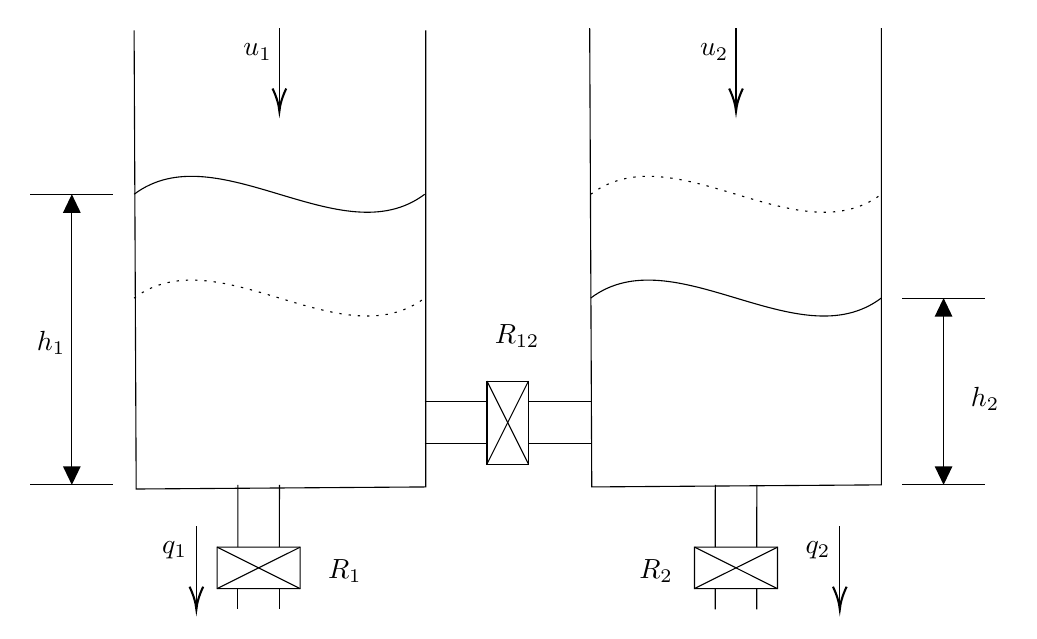
\begin{tikzpicture}[x=0.75pt,y=0.75pt,yscale=-1,xscale=1]
    %uncomment if require: \path (0,459); %set diagram left start at 0, and has height of 459
    %Straight Lines [id:da5688929335924803]
    \draw    (310.5,121) -- (310.5,341) -- (171,342) -- (170,121) ;
    %Straight Lines [id:da5444294116492245]
    \draw    (530,120) -- (530,340) -- (390.5,341) -- (389.5,120) ;
    %Straight Lines [id:da5805131124126722]
    \draw    (200,360) -- (200,398) ;
    \draw [shift={(200,400)}, rotate = 270] [color={rgb, 255:red, 0; green, 0; blue, 0 }  ][line width=0.75]    (10.93,-3.29) .. controls (6.95,-1.4) and (3.31,-0.3) .. (0,0) .. controls (3.31,0.3) and (6.95,1.4) .. (10.93,3.29)   ;
    %Straight Lines [id:da36945578968673487]
    \draw    (510,360) -- (510,398) ;
    \draw [shift={(510,400)}, rotate = 270] [color={rgb, 255:red, 0; green, 0; blue, 0 }  ][line width=0.75]    (10.93,-3.29) .. controls (6.95,-1.4) and (3.31,-0.3) .. (0,0) .. controls (3.31,0.3) and (6.95,1.4) .. (10.93,3.29)   ;
    %Straight Lines [id:da3077937138084411]
    \draw    (310,300) -- (340,300) ;
    %Straight Lines [id:da6773172185122848]
    \draw    (310,320) -- (340,320) ;
    %Shape: Rectangle [id:dp35476624369345366]
    \draw   (340,290) -- (360,290) -- (360,330) -- (340,330) -- cycle ;
    %Straight Lines [id:da9030142425581202]
    \draw    (360,300) -- (390,300) ;
    %Straight Lines [id:da9329287059080266]
    \draw    (360,320) -- (390,320) ;
    %Straight Lines [id:da7833363422326105]
    \draw    (340,290) -- (360,330) ;
    %Straight Lines [id:da26540765973372593]
    \draw    (360,290) -- (340,330) ;
    %Straight Lines [id:da7238601427391023]
    \draw    (470.02,340) -- (470,370) ;
    %Straight Lines [id:da21192498383993508]
    \draw    (450.02,339.99) -- (450,369.99) ;
    %Shape: Rectangle [id:dp4746471043409347]
    \draw   (480,370.01) -- (479.99,390.01) -- (439.99,389.98) -- (440,369.98) -- cycle ;
    %Straight Lines [id:da6336671048955647]
    \draw    (470,389.99) -- (469.98,400) ;
    %Straight Lines [id:da6700066277567417]
    \draw    (450,389.99) -- (449.98,400) ;
    %Straight Lines [id:da928718960478936]
    \draw    (480,370.01) -- (439.99,389.98) ;
    %Straight Lines [id:da1540497075962557]
    \draw    (479.99,390.01) -- (440,369.98) ;
    %Straight Lines [id:da7575667165517417]
    \draw    (240.03,340.01) -- (240.01,370.01) ;
    %Straight Lines [id:da24987185404211631]
    \draw    (220.03,340) -- (220.01,370) ;
    %Shape: Rectangle [id:dp2771887371908066]
    \draw   (250.01,370.02) -- (250,390.02) -- (210,389.99) -- (210.01,369.99) -- cycle ;
    %Straight Lines [id:da9912034440398235]
    \draw    (240,390) -- (240,400) ;
    %Straight Lines [id:da11904000202181764]
    \draw    (220,390) -- (220,400) ;
    %Straight Lines [id:da7480508238760858]
    \draw    (250.01,370.02) -- (210,389.99) ;
    %Straight Lines [id:da7049908339863217]
    \draw    (250,390.02) -- (210.01,369.99) ;
    %Straight Lines [id:da9101133488343268]
    \draw    (240,120) -- (240,158) ;
    \draw [shift={(240,160)}, rotate = 270] [color={rgb, 255:red, 0; green, 0; blue, 0 }  ][line width=0.75]    (10.93,-3.29) .. controls (6.95,-1.4) and (3.31,-0.3) .. (0,0) .. controls (3.31,0.3) and (6.95,1.4) .. (10.93,3.29)   ;
    %Straight Lines [id:da11474588029910615]
    \draw    (460,120) -- (460,158) ;
    \draw [shift={(460,160)}, rotate = 270] [color={rgb, 255:red, 0; green, 0; blue, 0 }  ][line width=0.75]    (10.93,-3.29) .. controls (6.95,-1.4) and (3.31,-0.3) .. (0,0) .. controls (3.31,0.3) and (6.95,1.4) .. (10.93,3.29)   ;
    %Curve Lines [id:da10596831311641142]
    \draw    (170,200) .. controls (210,170) and (270,230) .. (310,200) ;
    %Curve Lines [id:da32042097611565956]
    \draw    (390,250) .. controls (430,220) and (490,280) .. (530,250) ;
    %Curve Lines [id:da9628648357071894]
    \draw  [dash pattern={on 0.84pt off 2.51pt}]  (170,250) .. controls (210,220) and (270,280) .. (310,250) ;
    %Curve Lines [id:da13605436176729158]
    \draw  [dash pattern={on 0.84pt off 2.51pt}]  (390,200) .. controls (430,170) and (490,230) .. (530,200) ;
    %Straight Lines [id:da6375240487876032]
    \draw    (140,202) -- (140,338) ;
    \draw [shift={(140,340)}, rotate = 270] [fill={rgb, 255:red, 0; green, 0; blue, 0 }  ][line width=0.75]  [draw opacity=0] (8.93,-4.29) -- (0,0) -- (8.93,4.29) -- cycle    ;
    \draw [shift={(140,200)}, rotate = 90] [fill={rgb, 255:red, 0; green, 0; blue, 0 }  ][line width=0.75]  [draw opacity=0] (8.93,-4.29) -- (0,0) -- (8.93,4.29) -- cycle    ;
    %Straight Lines [id:da08454244898673535]
    \draw    (120,200) -- (160,200) ;
    %Straight Lines [id:da6622529040678575]
    \draw    (120,340) -- (160,340) ;
    %Straight Lines [id:da8094387172838741]
    \draw    (560,252) -- (560,338) ;
    \draw [shift={(560,340)}, rotate = 270] [fill={rgb, 255:red, 0; green, 0; blue, 0 }  ][line width=0.75]  [draw opacity=0] (8.93,-4.29) -- (0,0) -- (8.93,4.29) -- cycle    ;
    \draw [shift={(560,250)}, rotate = 90] [fill={rgb, 255:red, 0; green, 0; blue, 0 }  ][line width=0.75]  [draw opacity=0] (8.93,-4.29) -- (0,0) -- (8.93,4.29) -- cycle    ;
    %Straight Lines [id:da5524739963534533]
    \draw    (540,250) -- (580,250) ;
    %Straight Lines [id:da7800336719151444]
    \draw    (540,340) -- (580,340) ;
    % Text Node
    \draw (189.5,371.5) node  [align=left] {$\displaystyle q_{1}$};
    % Text Node
    \draw (499.5,371.5) node  [align=left] {$\displaystyle q_{2}$};
    % Text Node
    \draw (354.5,268.5) node  [align=left] {$\displaystyle R_{12}$};
    % Text Node
    \draw (229.5,131.5) node  [align=left] {$\displaystyle u_{1}$};
    % Text Node
    \draw (449.5,131.5) node  [align=left] {$\displaystyle u_{2}$};
    % Text Node
    \draw (130,271.5) node  [align=left] {$\displaystyle h_{1}$};
    % Text Node
    \draw (580,298.5) node  [align=left] {$\displaystyle h_{2}$};
    % Text Node
    \draw (271.5,381.5) node  [align=left] {$\displaystyle R_{1}$};
    % Text Node
    \draw (421.5,381.5) node  [align=left] {$\displaystyle R_{2}$};
  \end{tikzpicture}%
  }
  \caption[System of Coupled Tanks.]{System of Coupled Tanks. Two pumps input
    water into the system, and the water can flow out of the system through each
    tank. The water can also flow from one tank to another, making the state of
    one affect the state of the other. The control objective are the water
    levels of both tanks. The solid and dashed lines representing the water
    levels illustate two configurations, one with \(h_{1}>h_{2}\) and the
    contrary.}%
  \label{fig:tanks-sim}
\end{figure}


The output flow of the \(T1\) and \(T2\) are denoted by \(q_1\) and \(q_2\)
(\si{\cubic\centi\metre\per\second}), respectively, and the flow between them is
noted by \(q_{12}\) (\si{\cubic\centi\metre\per\second}). Both tanks have the
same cross-section area, denoted as \(A\) (\si{\square\centi\metre}), as well as the
cross-section areas of the restrictions in the outputs of the tanks, \(a\)
(\si{\square\centi\metre}); \(g\) (\si{\centi\metre\per\square\second}) is the gravity
acceleration. By using Bernoulli's equations, we have:
%
\begin{equation}
  \label{eq:formula-height-variation-lin}
  \begin{aligned}
    \dot{h}_1(t) & = \frac{u_1(t)-q_1(t)\pm{}q_{12}}{A}, \\
    \dot{h}_2(t) & = \frac{u_2(t)-q_2(t)\mp{}q_{12}}{A},
  \end{aligned}
\end{equation}
%
where the flows are given by \(q_1(t) = a\sqrt{2gh_1(t)}\),
\(q_2(t) = a\sqrt{2gh_2(t)}\), and
\(q_{12}(t) = a\sqrt{2g\left|h_2(t)-h_1(t)\right|}\).

This is a nonlinear and switching system, as the model changes depending on the
height of the tanks' water column. At each mode, \(h_1>h_2\) or \(h_1\leq h_2\),
equation~\eqref{eq:formula-height-variation-lin} can be linearized around an
equilibrium operational point \((x_{eq},u_{eq})\) by using Jacobian matrices. In
what follows, we use \(a=\SI{5.9}{\centi\metre\squared}\),
\(A=\SI{961\pi{}}{\centi\metre\squared}\), and
\(g=\SI{980.665}{\centi\metre\per\square\second}\).

Two operational conditions with
\(x(k) = \begin{bmatrix}h_1(k) & h_2(k)\end{bmatrix}^\top{}\), chosen so one tank
is nearly full, are such that:
%
\begin{equation*}
  x_{eq}^1 =\! \begin{bmatrix}
    57.5 \\ 43.61
  \end{bmatrix}\!,
  u_{eq}^1 =\! \begin{bmatrix}
    744 \\ 2960
  \end{bmatrix}\!,
  x_{eq}^2 = \begin{bmatrix}
    43.61 \\ 57.5
  \end{bmatrix}\!,
  u_{eq}^2 =\! \begin{bmatrix}
    2960 \\ 744
  \end{bmatrix}\!,
\end{equation*}
%
yielding two operational modes, each of them corresponding to a \CG{}.\@
%
After the linearization, we discretized the continuous-time model using a sample
time of \SI{5}{\second} and Euler equations to get discrete-time model given
by~\eqref{eq:state-space} with matrices:
%
\begin{align*}
  A_1 & =
  \begin{bmatrix}
    0.92  & 0.053 \\
    0.053 & 0.91
  \end{bmatrix}, ~~~ A_2 = \begin{bmatrix}
    0.91  & 0.053 \\
    0.053 & 0.92
  \end{bmatrix} \\
  B_1 & =
  \begin{bmatrix}
    0.0016           & 4.5\times10^{-5} \\
    4.5\times10^{-5} & 0.0016
  \end{bmatrix},
  B_2 = \begin{bmatrix}
    0.0016           & 4.5\times10^{-5} \\
    4.5\times10^{-5} & 0.0016
  \end{bmatrix},                              \\
  %
  C_1 & = C_2 =
  \begin{bmatrix}
    1 & 0 \\
    0 & 1
  \end{bmatrix},
\end{align*}
%
and number of modes \(s=2\). Using Lyapunov's
approach~\parencite{chen:linear,hespanha:linear}, on the system augmented with 2
integrators (one for each state), we got the following controller:
%
\begin{align*}
  K_1 & = \begin{bmatrix}
    -875.384 & -9.217   & -297.447 & 7.982    \\
    -8.505   & -849.853 & 8.514    & -279.434
  \end{bmatrix}, \\
  %
  K_2 & = \begin{bmatrix}
    -849.853 & -8.505   & -279.434 & 8.514    \\
    -9.217   & -875.384 & 7.982    & -297.447
  \end{bmatrix},
\end{align*}
%
for the operational modes \(1\) and \(2\).

We simulated our approaches described by Algorithm~\ref{alg:roa-rule} to switch
between the \CG{}s 1 and 2. In both cases the system starts in \(x(0) =
\begin{bsmallmatrix}43.61 & 57.5\end{bsmallmatrix}^{\top}\). The references are
\(r = \begin{bsmallmatrix}57.5 & 43.61\end{bsmallmatrix}^{\top}\), for
\(0\leq k\leq 10 \cup 50 \leq k \leq\infty{}\), and
\(r = \begin{bsmallmatrix}43.61& 57.5\end{bsmallmatrix}^{\top}\), for
\(11 \leq k \leq 49\). Therefore, the system must perform a closed path. Note that the
references are the system's two equilibrium points, so the systems starts in
mode 1, moves to mode 2 and goes back to mode 1.

The regions of attraction were estimated using the optimization procedure
presented in Section~\ref{sec:region-of-attraction}. The following inequalities
define each mode's regions of attraction:
%
\begin{align}
  \mathcal{L}_{V_{1}}(x) & = x^{\top} \begin{bmatrix}
    4.766\times{}10^{-3} & 1.431\times{}10^{-8} \\
    1.431\times{}10^{-8} & 4.766\times{}10^{-3}
  \end{bmatrix}x \leq 1 \\
  \mathcal{L}_{V_{2}}(x) & = x^{\top} \begin{bmatrix}
    4.766\times{}10^{-3} & 1.185\times{}10^{-8} \\
    1.185\times{}10^{-8} & 4.766\times{}10^{-3}
  \end{bmatrix}x \leq 1
\end{align}

The constraint regions are, in this case, also defined as ellipses, given by the
following inequalities:
%
\begin{align}
  \mathcal{C}_{1}(x) & = \frac{(x_{1}-50.55)^{2}}{8.681^{2}} + \frac{(x_{2}-43.61)^{2}}{1.085^{2}} \leq 1 \\
  \mathcal{C}_{2}(x) & = \frac{(x_{1}-43.61)^{2}}{1.085^{2}} + \frac{(x_{2}-50.55)^{2}}{8.681^{2}} \leq 1
\end{align}
%
where \(x=\begin{bsmallmatrix} x_{1} & x_{2} \end{bsmallmatrix}^{\top}\).

Since the system is linearized around two different operation points, there are
three bases (the equilibrium points of each linearized model), and the states
need to be converted between them. The first is the basis of the non-linear
system, called \enquote{global}. The second and third are those of the
linearized systems. The constraints are written on the global basis and the
regions of attraction in the respective mode's basis. Care must be taken to
convert between the basis for set membership tests.

Fig.~\ref{fig:states} shows the path taken by the closed-loop system over the
space of the system's state. The trajectory marked with
\textcolor{red}{red-dashed line} concerns the results achieved without
early-switch, and the \textcolor{blue}{solid-blue line} is related to ones with
early-switch. The shadow regions concern the constraints of each mode. Also,
Fig.~\ref{fig:states} shows the borders of the estimates of the regions of
attraction, RoA, for each mode, with dot-dashed lines.

It is clear that the path taken under each algorithm's variation (with and
without early controller switch) are almost the same. The respective control
signals are given in Fig.~\ref{fig:control-signals}, showing faster convergence
and smaller signal amplitude in the hybrid switch.

\begin{figure}[ht!]
  \centering
  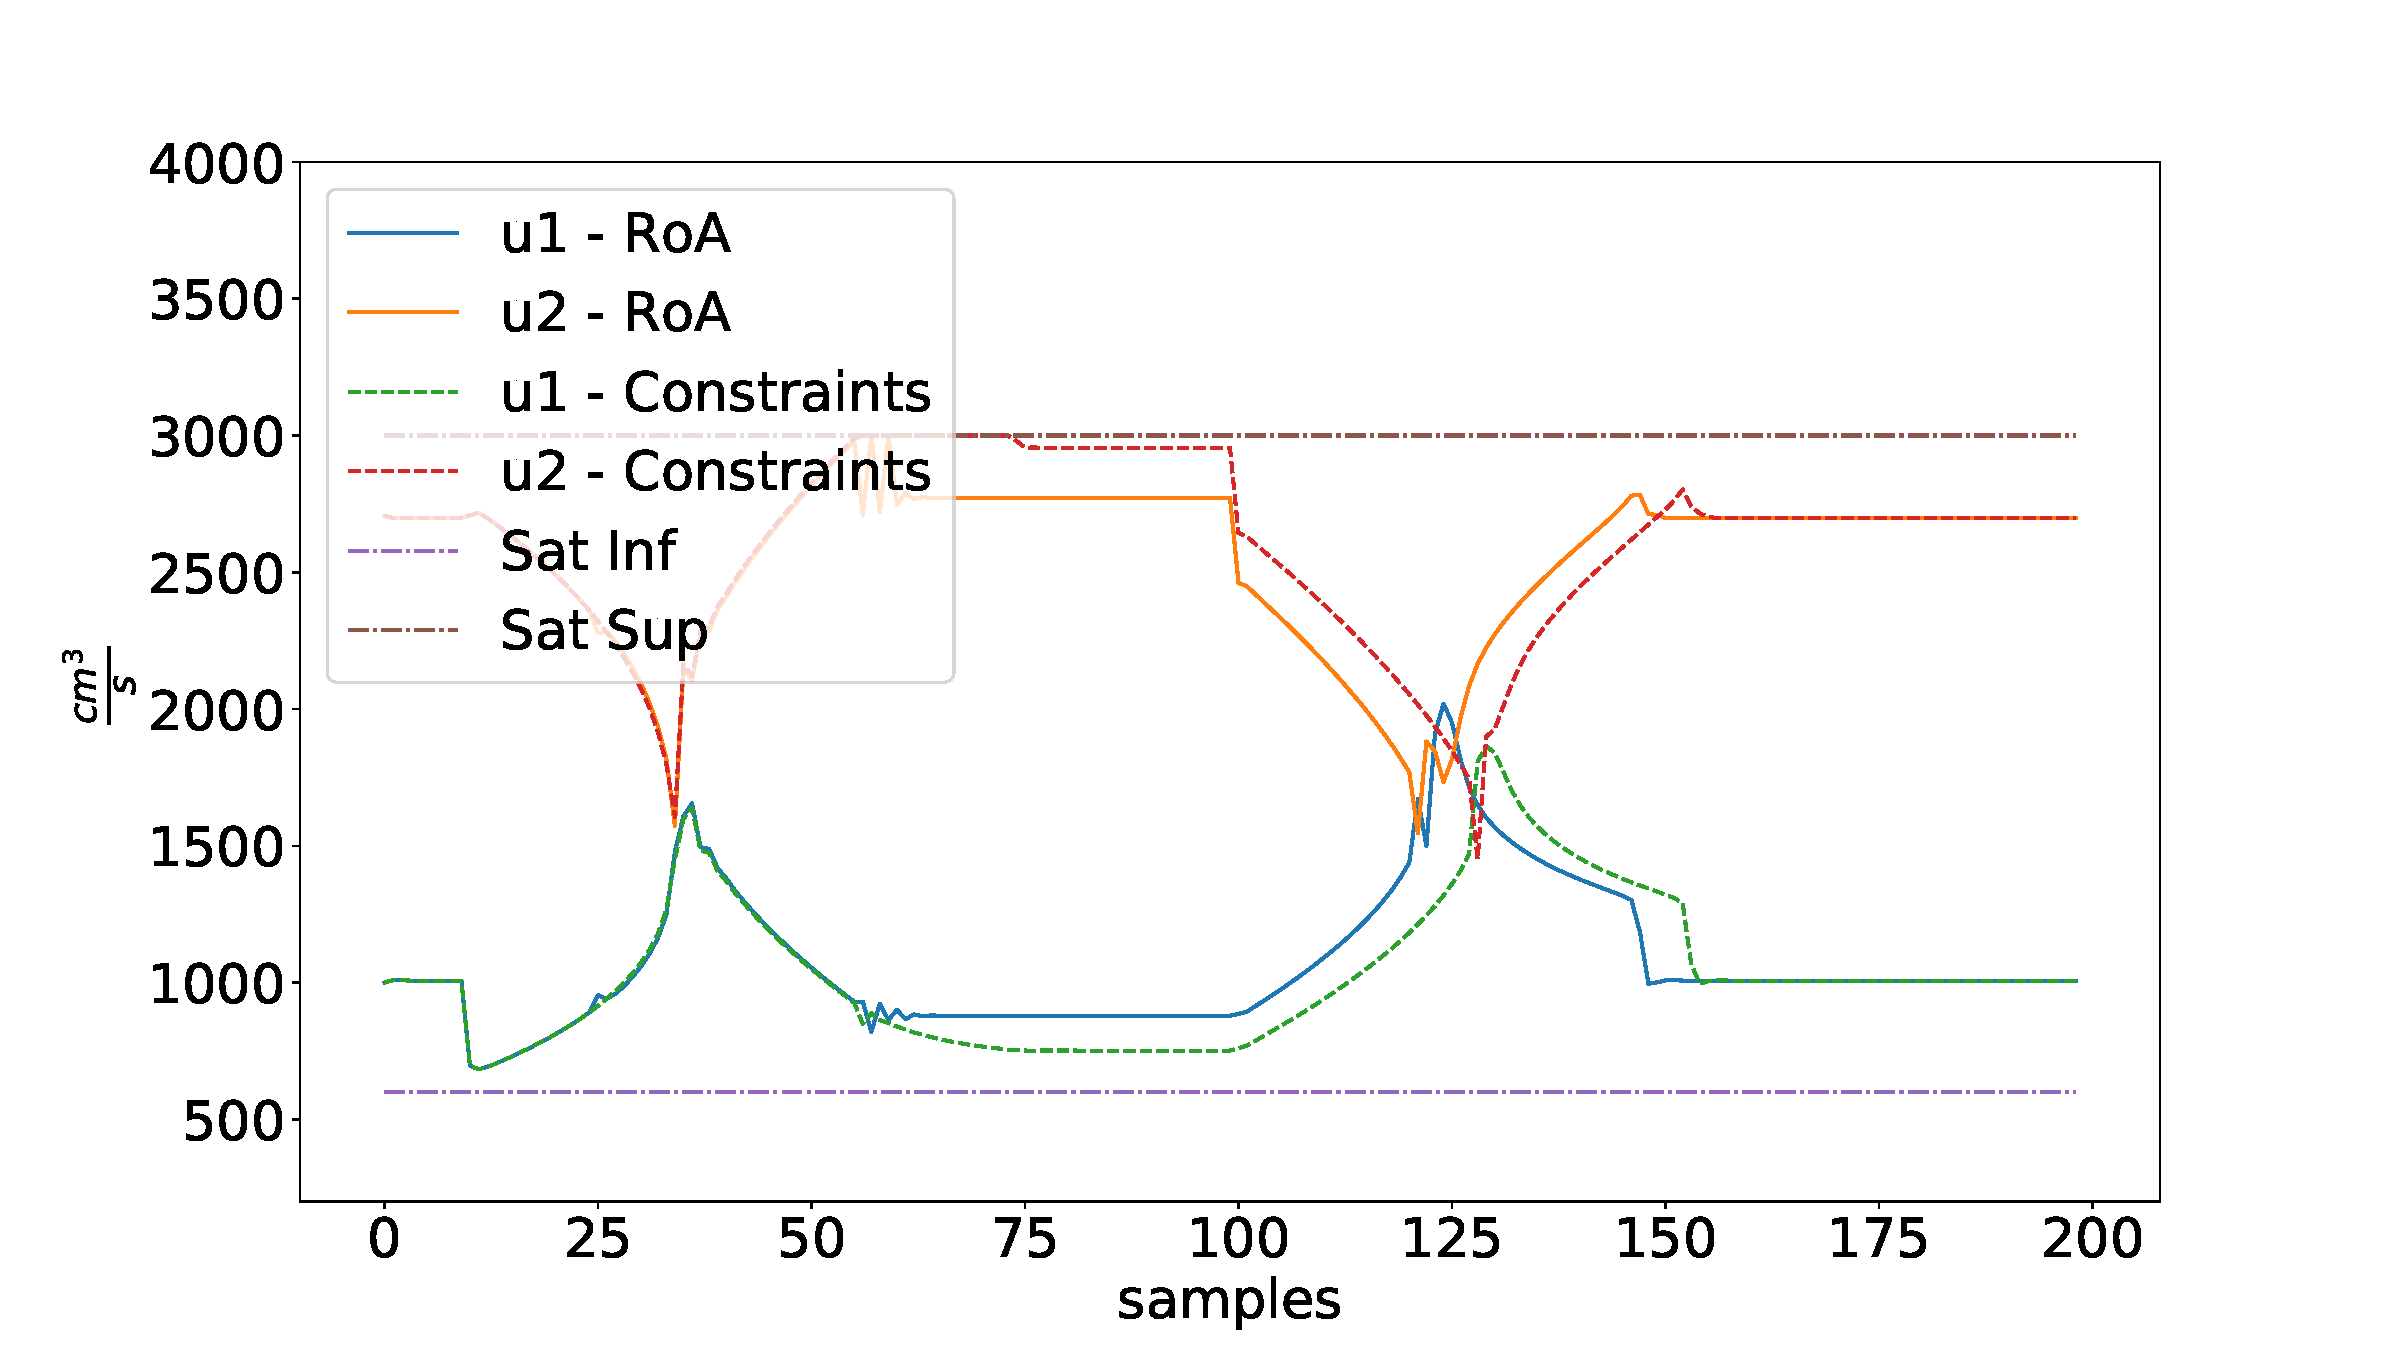
\includegraphics[width=0.8\linewidth]{imgs/tanks-control-signal}
  \caption[Control signals for Example 1.]{Control signals for Example 1. Solid
    lines are the hybrid switch and dashed lines are the normal switch.
    Dashed-dotted lines are saturations.}%
  \label{fig:control-signals}
\end{figure}

\begin{figure}[ht!]
  \centering
  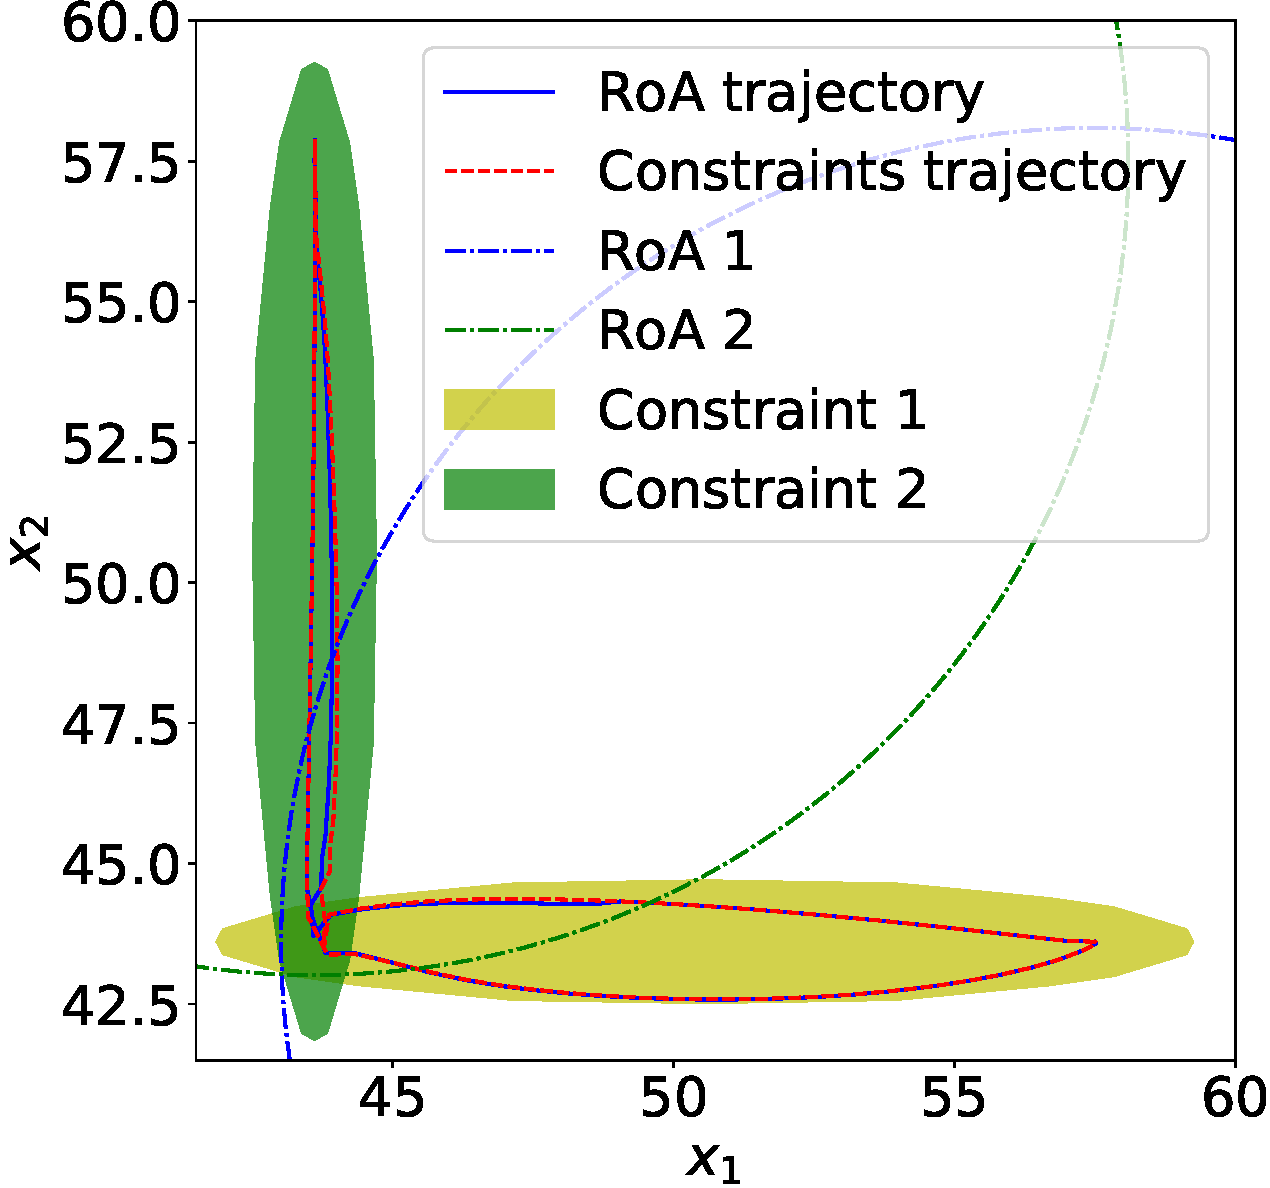
\includegraphics[width=0.9\linewidth]{imgs/tanks-states}
  \caption[States trajectory for Example 1.]{States trajectory for Example 1.
    The filled ellipses are each mode's constraints. The dashed-dotted circles
    are each controller's Region of Attraction. The dashed blue red line is the
    state path of the normal switch and the solid blue line the state path of
    the hybrid switch.}%
  \label{fig:states}
\end{figure}

\FloatBarrier

\subsection{Unstable System}%
\label{subsec:unstable-system}

Consider the unstable switching system with matrices
%
\begin{align*}
  A_1 & =
  \begin{bmatrix}
    1 & 0.003 \\
    0 & 1
  \end{bmatrix},
  A_2 = \begin{bmatrix}
    1 & 0.0074 \\
    0 & 1.1
  \end{bmatrix}, \\
  B_1 & =
  \begin{bmatrix}
    0.0005 & 1.2\times{}10^{-6} \\
    0      & 0.0008
  \end{bmatrix},
  B_2 = \begin{bmatrix}
    0.0019 & 3.6\times{}10^{-5} \\
    0      & 0.011
  \end{bmatrix}, \\
  %
  C_1 & = C_2 =
  \begin{bmatrix}
    1 & 0 \\
    0 & 1
  \end{bmatrix},       \\
\end{align*}
%
and operational points
%
\[
  x_{eq}^1 = \begin{bmatrix}
    1 \\ 1
  \end{bmatrix},
  u_{eq}^1 = \begin{bmatrix}
    -2 \\ \frac{-5}{4}
  \end{bmatrix},
  x_{eq}^2 = \begin{bmatrix}
    -1 \\ 1
  \end{bmatrix},
  u_{eq}^2 = \begin{bmatrix}
    \frac{-30}{19} \\ -10
  \end{bmatrix}.
\]
%
The sample-period was \SI{0.1}{\second}, and controller gains are given by:
%
\scriptsize
\begin{align*}
  K_1 & = \begin{bmatrix}
    -2.669\times{}10^3   & -1.993             & -6.741\times{}10^2    & 1.010              \\
    3.582\times{}10^{-4} & -1.669\times{}10^3 & -3.103\times{}10^{-4} & -4.210\times{}10^2
  \end{bmatrix}, \\
  %
  K_2 & = \begin{bmatrix}
    -7.034\times{}10^2    & -1.268             & -1.769\times{}10^2    & 6.097\times{}10^{-1} \\
    -3.903\times{}10^{-6} & -1.370\times{}10^2 & -1.292\times{}10^{-5} & -3.202\times{}10^1
  \end{bmatrix}.
\end{align*}
\normalsize

With the same procedures and considerations of the previous example, including
the used color codes, we simulated the unstable system.
Figure~\ref{fig:unstable-states} shows the same system trajectory for both
methods.

\begin{figure}[ht!]
  \centering
  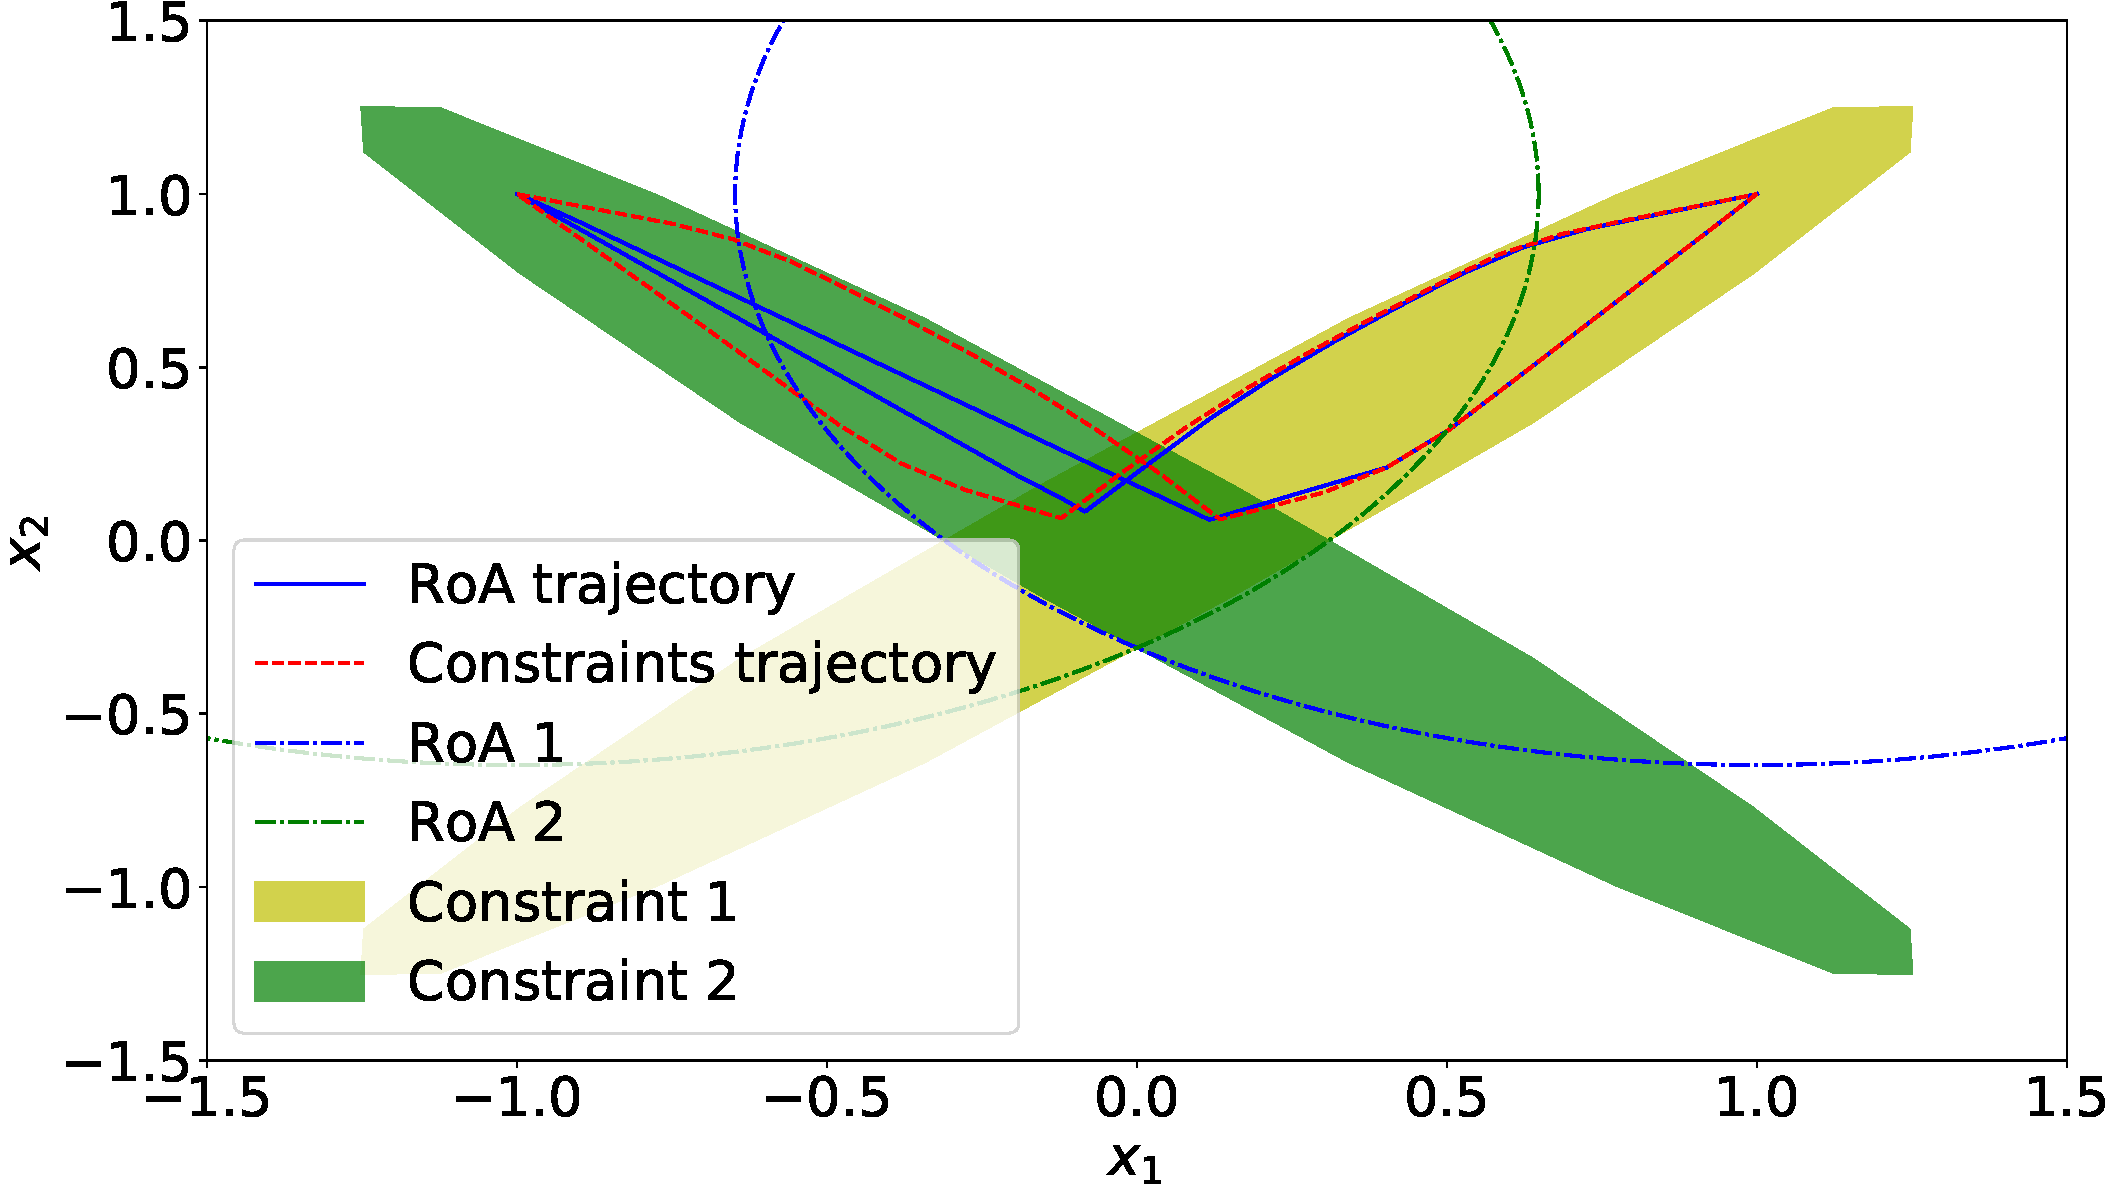
\includegraphics[width=\linewidth]{imgs/unstable_states}
  \caption[States trajectory for Example 2.]{States trajectory for Example 2.
    The filled ellipses are each mode's constraints. The dashed-dotted circles
    are each controller's Region of Attraction. The dashed blue red line is the
    state path of the normal switch and the solid blue line the state path of
    the hybrid switch.}%
  \label{fig:unstable-states}
\end{figure}

The second method shows better performance under control signal restrictions.
Figure~\ref{fig:unstable-control-signals} reveals a difference in the control
signals, where the first method, displayed in \textcolor{red}{red dashed-line}
and \textcolor{green}{green dashed-line}, have higher control signal outputs
than the second method, shown by \textcolor{blue}{blue solid-line} and
\textcolor{orange}{orange solid-line}. Both methods results in the same settling
time, but with much lower control effort with the strategy of early switching.

\begin{figure}[ht!]
  \centering
  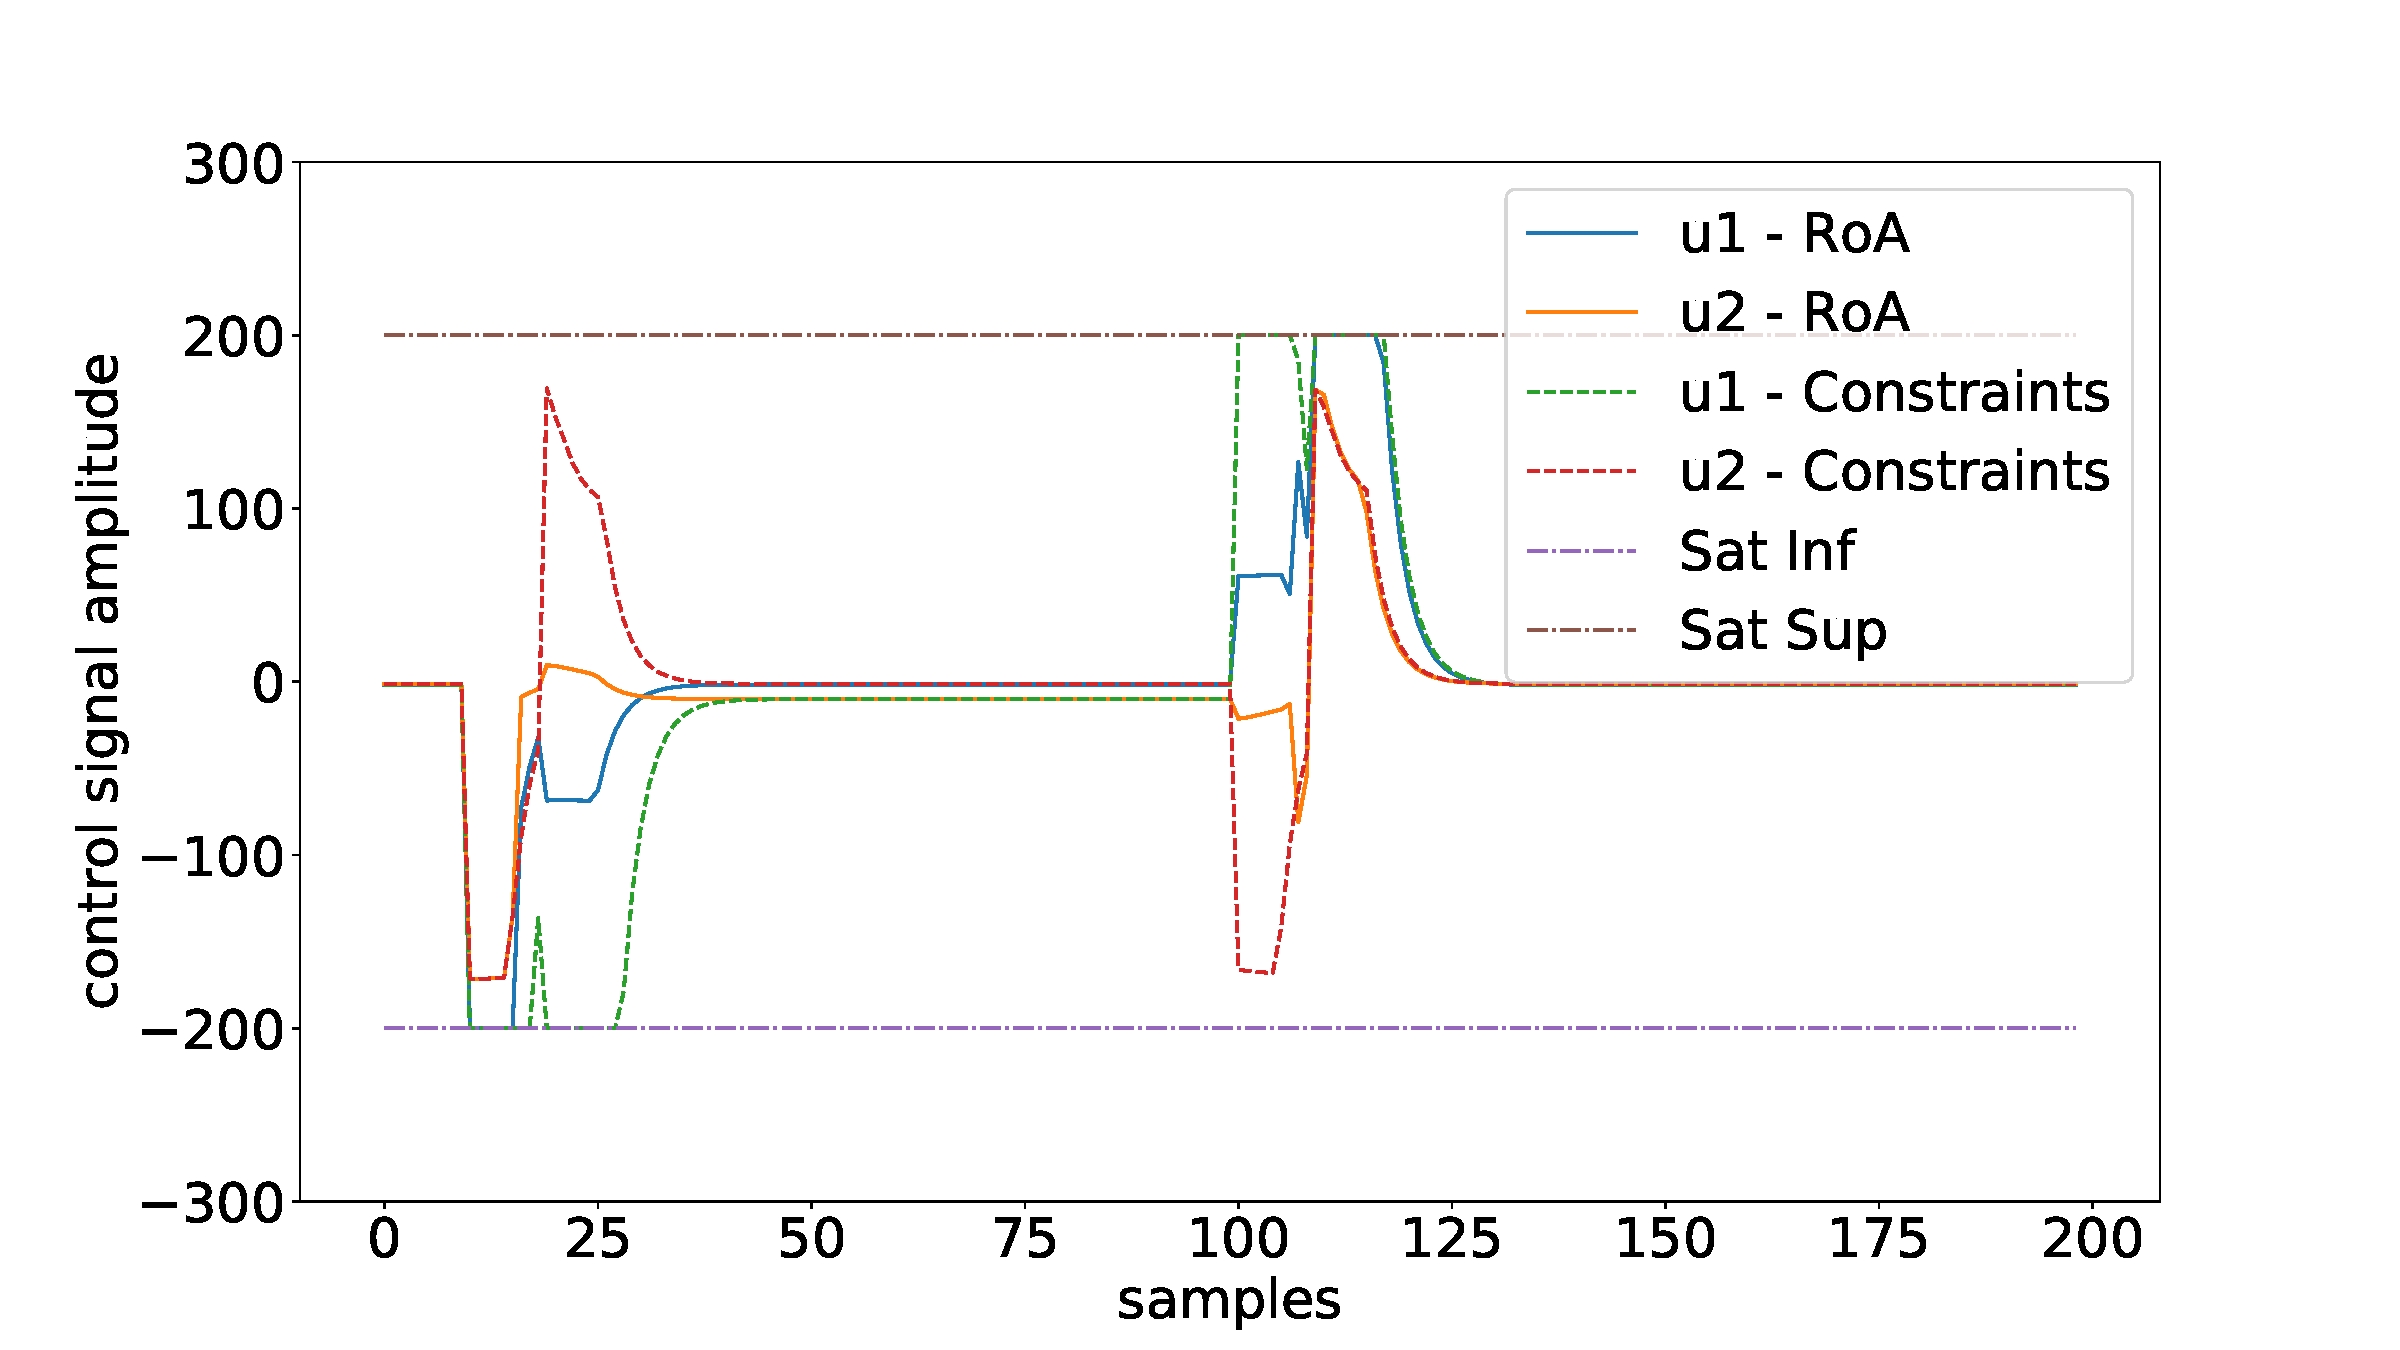
\includegraphics[width=\linewidth]{imgs/unstable_control_signal}
  \caption[Control signals for Example 2.]{Control signals for Example 2. Solid
    lines are the hybrid switch and dashed lines are the normal switch.
    Dashed-dotted lines are saturations.}%
  \label{fig:unstable-control-signals}
\end{figure}

\FloatBarrier

\subsection{Cessna 182}%
\label{subsec:cessna}

\textcite{franzè.lucia.ea:command} present a Cessna 182 aircraft model, which
they used to simulate a dwell-time. They describe the model, the operation
points they chose, and the constraints applied to it. We used the same system
changing only the switch technique to compare the performance. The proposed
technique took \SI{6}{\second} to converge, whereas the dwell-time technique
took over \SI{20}{\second}.

Figure~\ref{fig:cessna-u} shows both actuators' control signals, which are kept
mostly invariant, except at the mode transitions, where the integrator reset
created a discontinuity. Figure~\ref{fig:cessna-x} shows each state. In both
figures, the solid black lines at the plot's top and bottom are the signal's
constraints. The last state (\(x_{4}\)) is the output, and its plot also shows
the reference and command governor's output.

\begin{figure}[ht!]
  \centering
  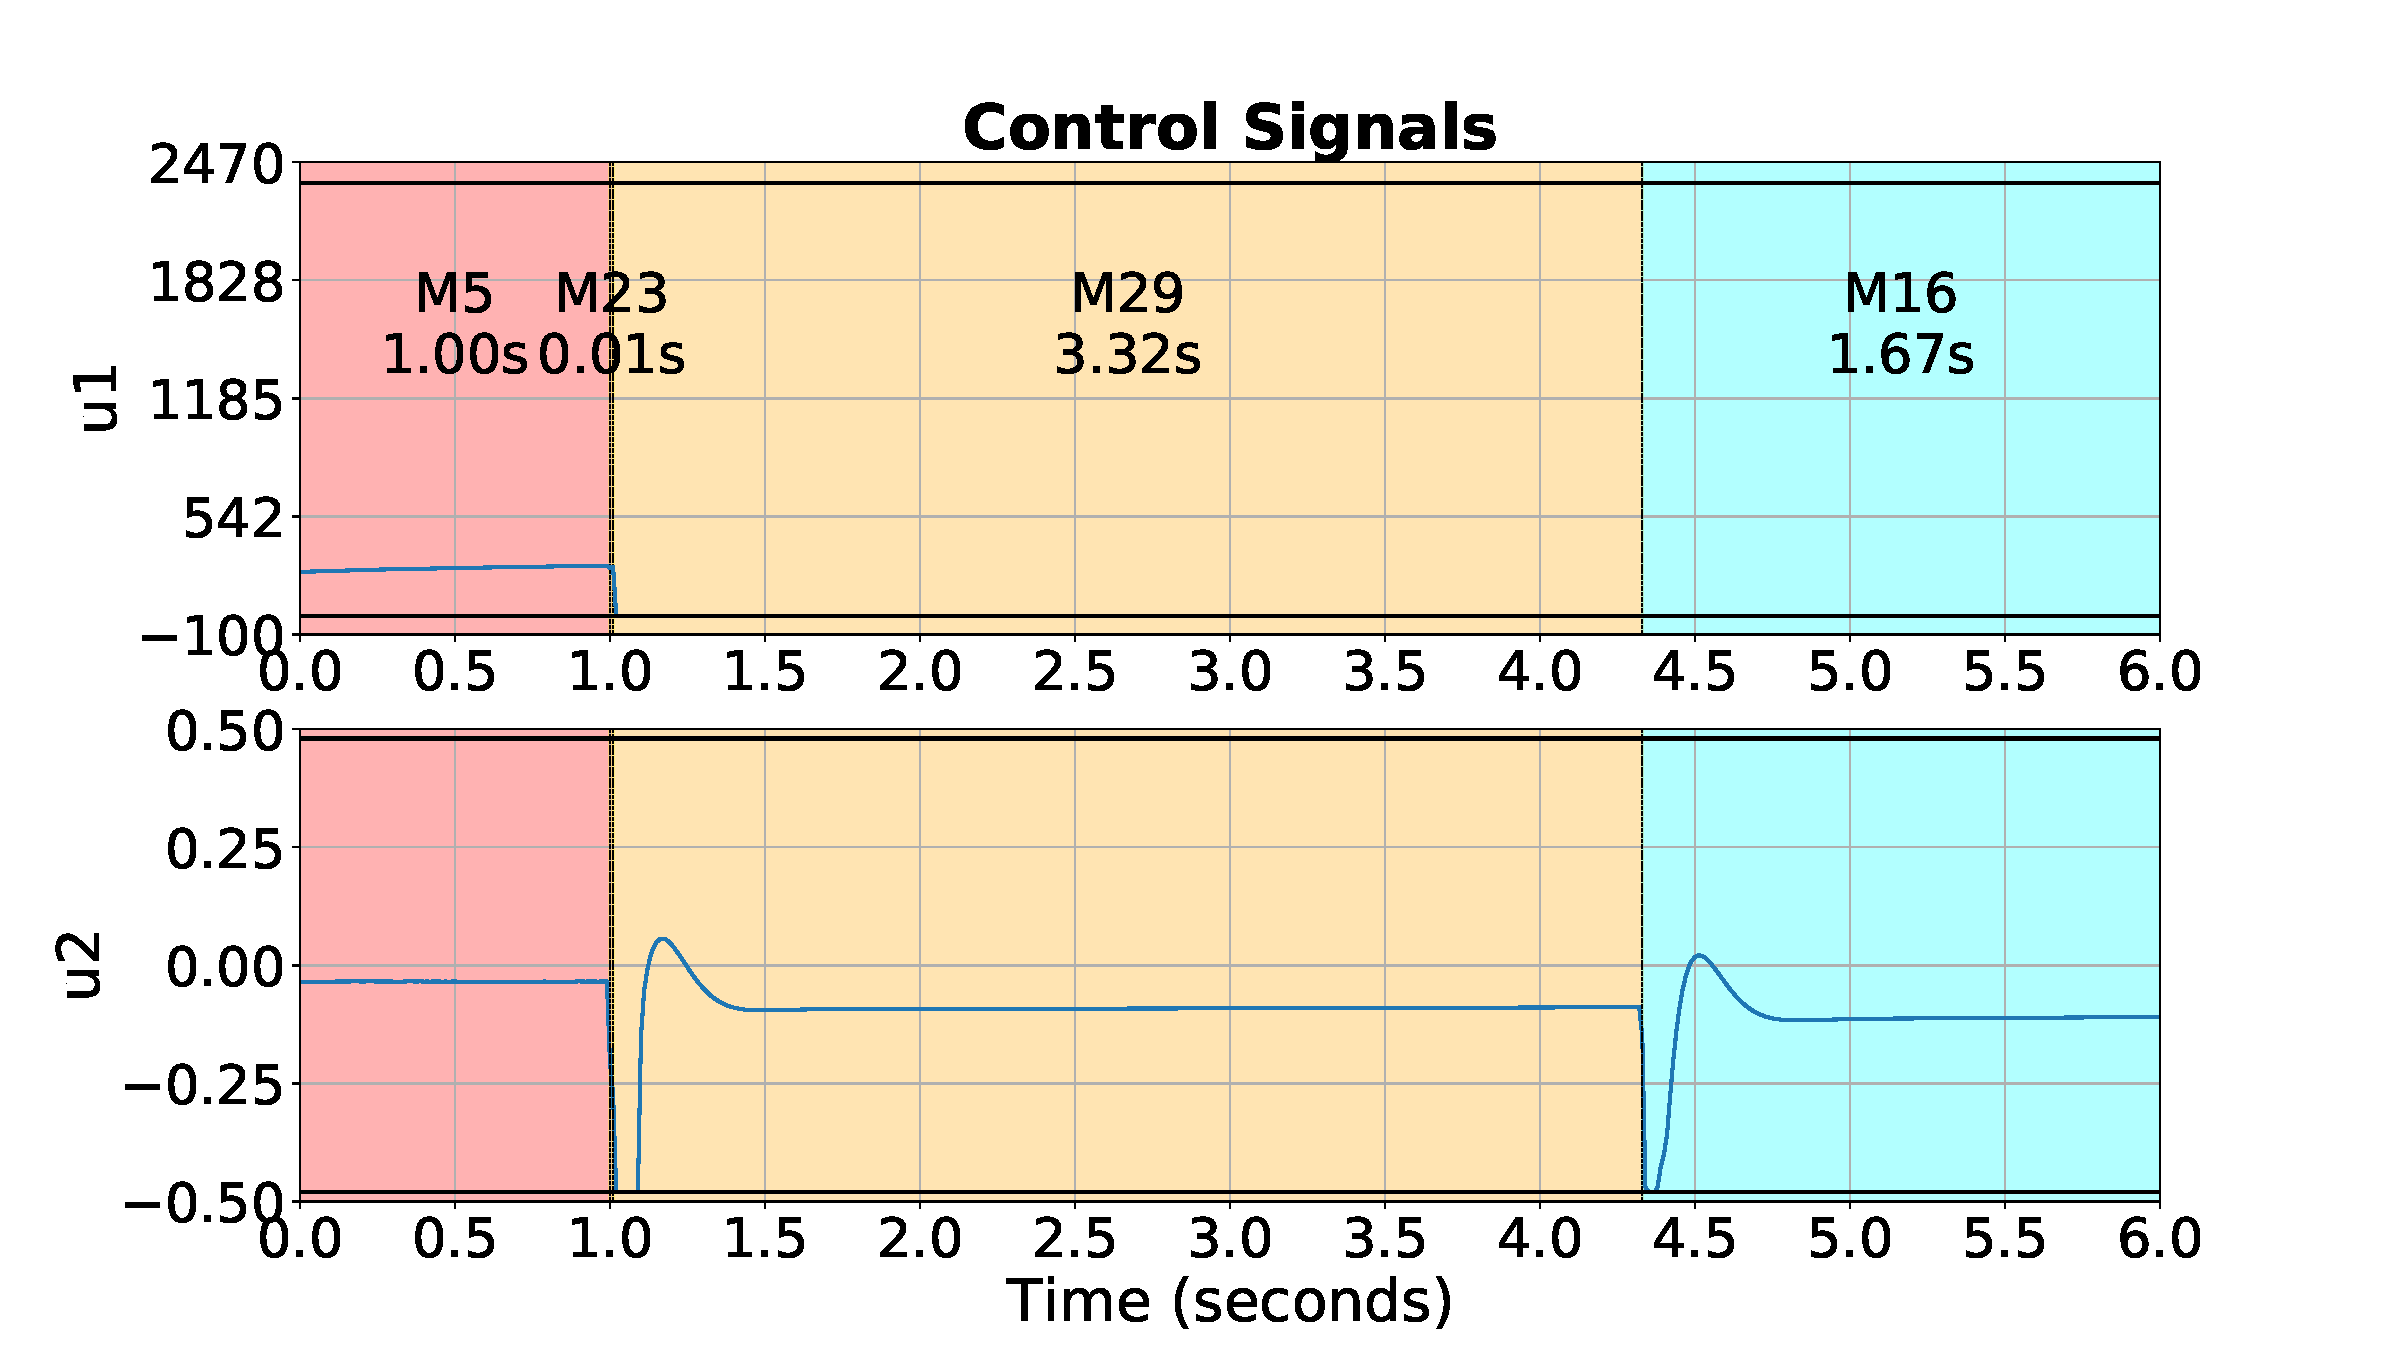
\includegraphics[height=0.3\textheight]{imgs/cessna-u}
  \caption{Cessna 192 control signals.}%
  \label{fig:cessna-u}
\end{figure}

\begin{figure}[ht!]
  \centering
  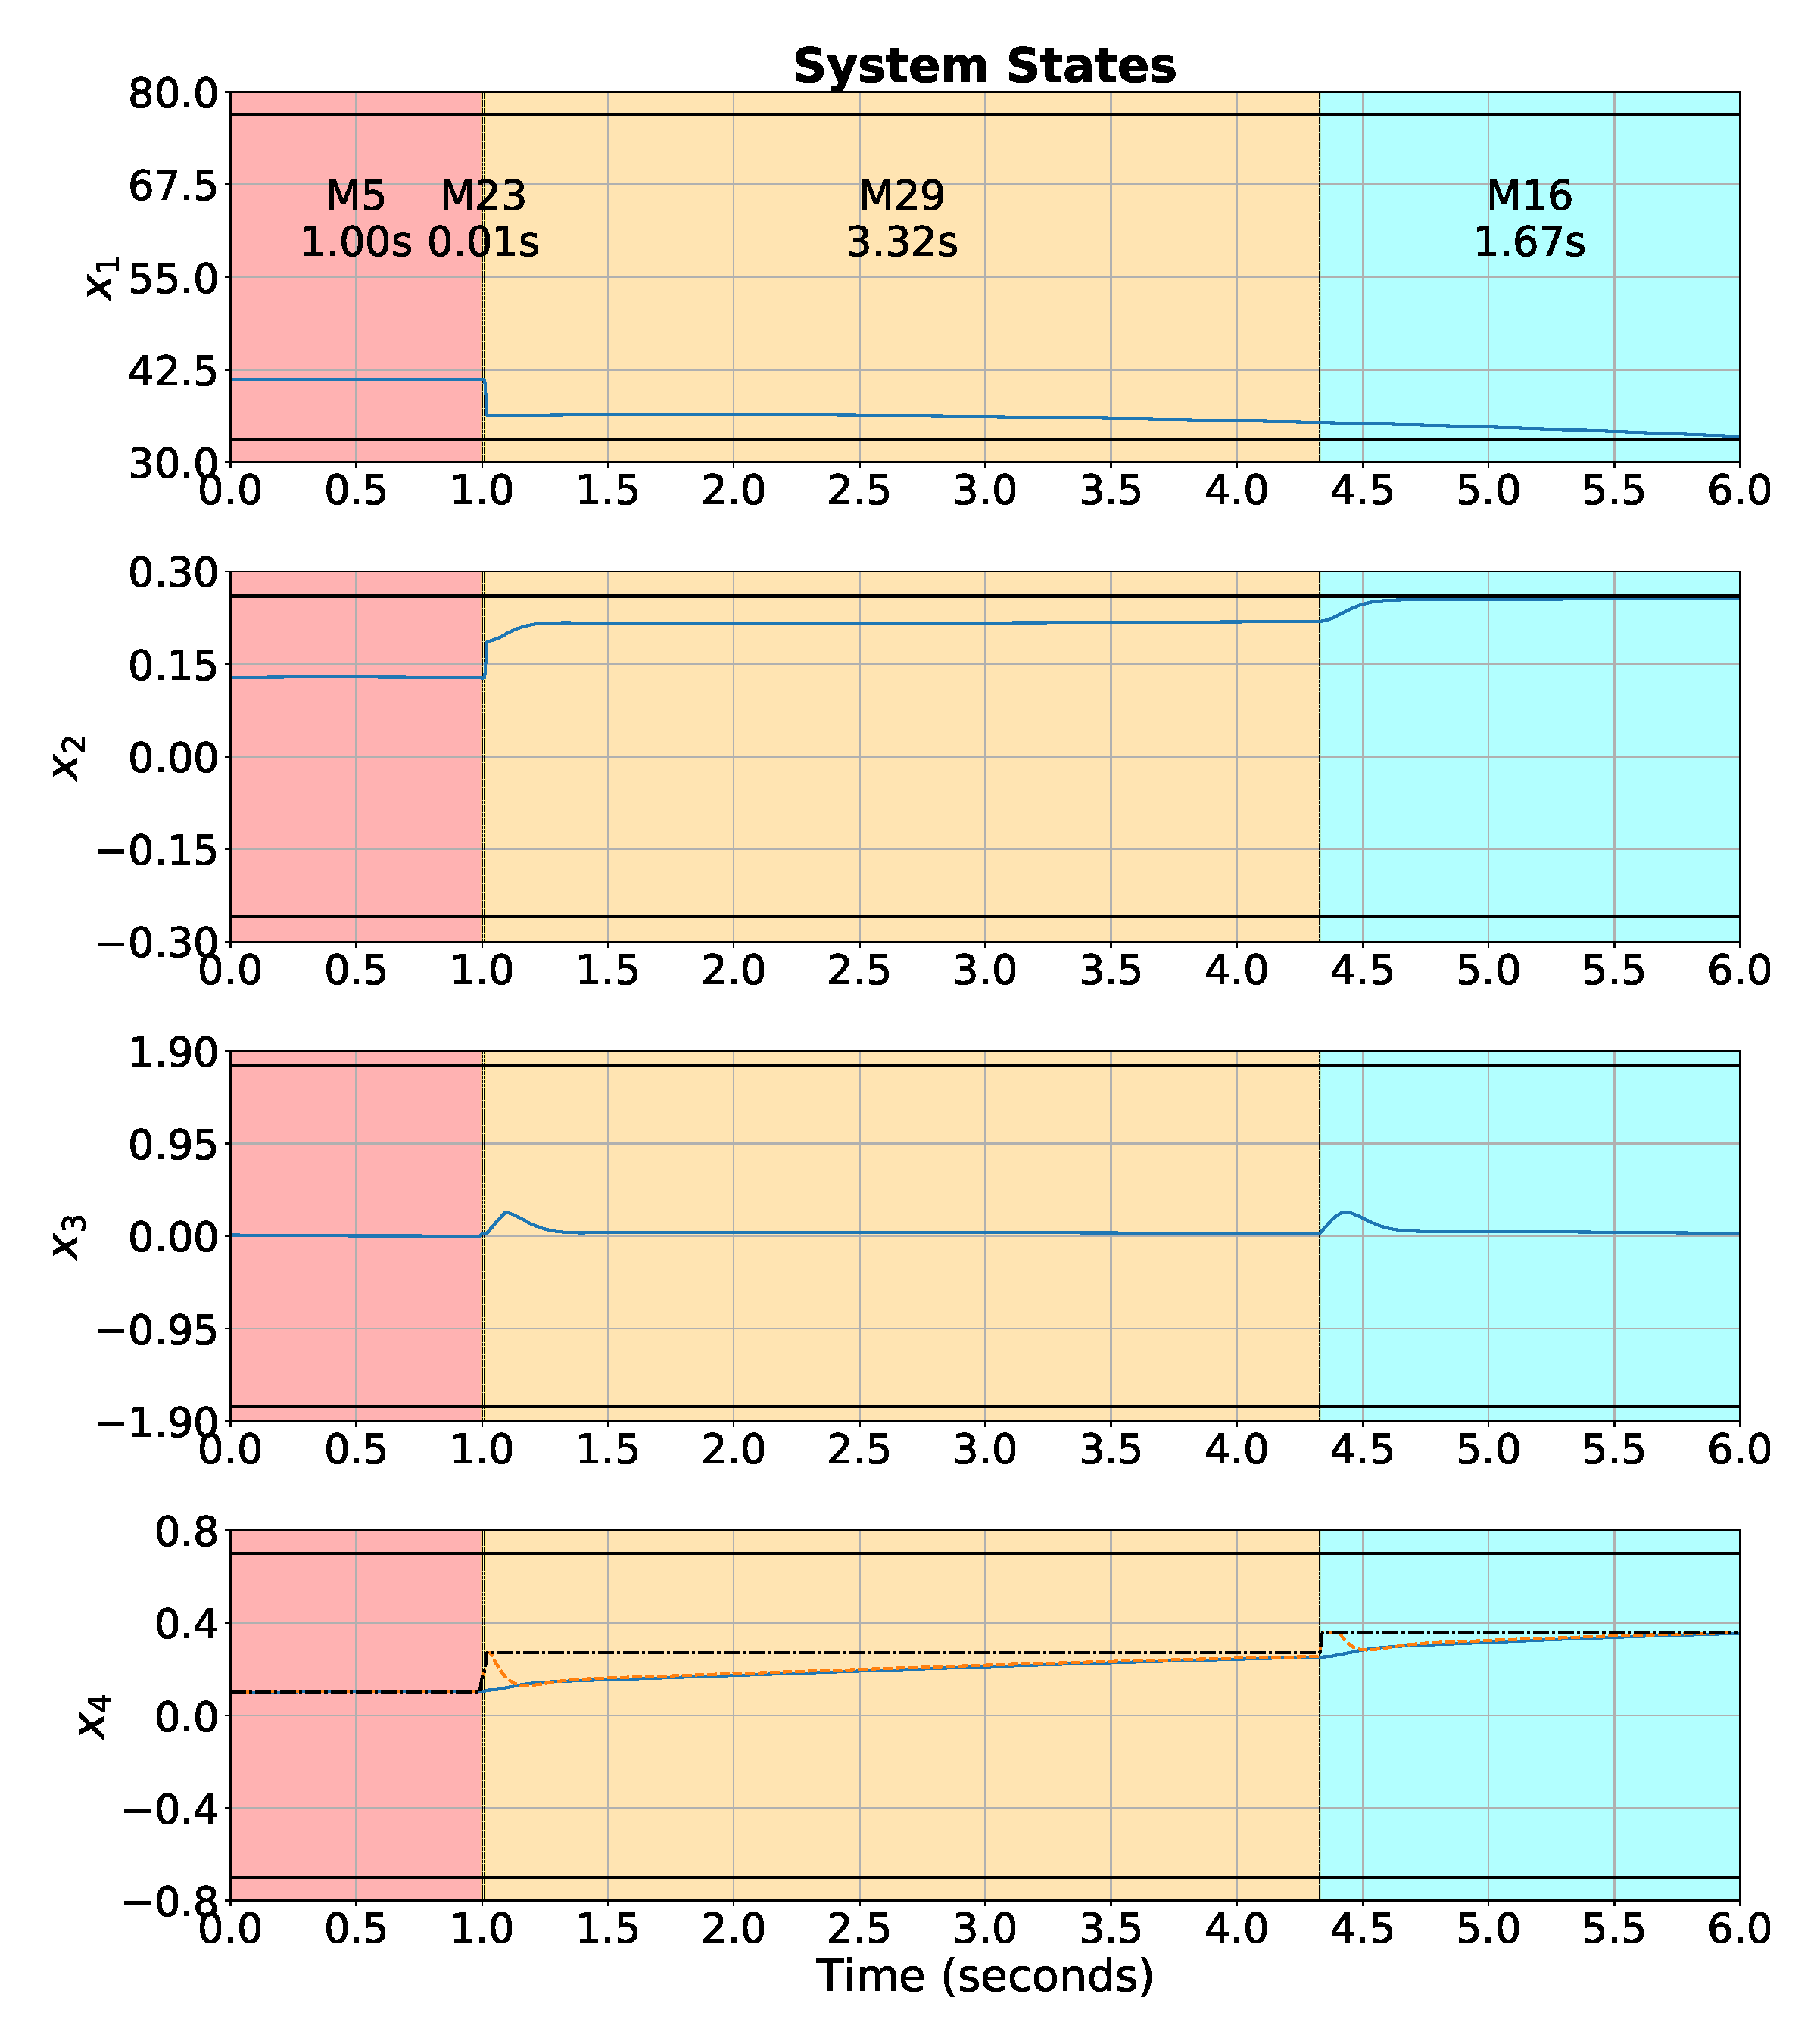
\includegraphics[height=0.6\textheight]{imgs/cessna-x}
  \caption[Cessna 182 states.]{Cessna 182 states. The colored backgrounds show
    the active mode. In the last plot, the dashed black line is the reference
    set by the supervisor, the dashed orange line is the reference generated by
    the Command Governor, the solid blue line is the state and the solid black
    lines are the saturation values.}%
  \label{fig:cessna-x}
\end{figure}

\section{Experimental Results}%
\label{sec:experimental-results}

Consider an interactive tank system as indicated in Figure~\ref{fig:tanks}. It
describes the physical system present at the System Analysis Laboratory of
CEFET-MG campus V, shown in Figure~\ref{fig:tanks-real}. It consists of two
coupled tanks, \(T1\) and \(T2\), that are fed by a pump with controlled flow
\(u(t)\), measured in \si{\cubic\centi\metre\per\second}. The levels of each
tank, \(h_1\) and \(h_2\) (\si{\centi\metre}), are the control objective
variables, and are measured
directly~\parencite{franco.oliveira.ea:síntese,sousa.leite.ea:affordable,lopes.leite.ea:anti-windup}.

\begin{figure}[ht!]
  \centering
  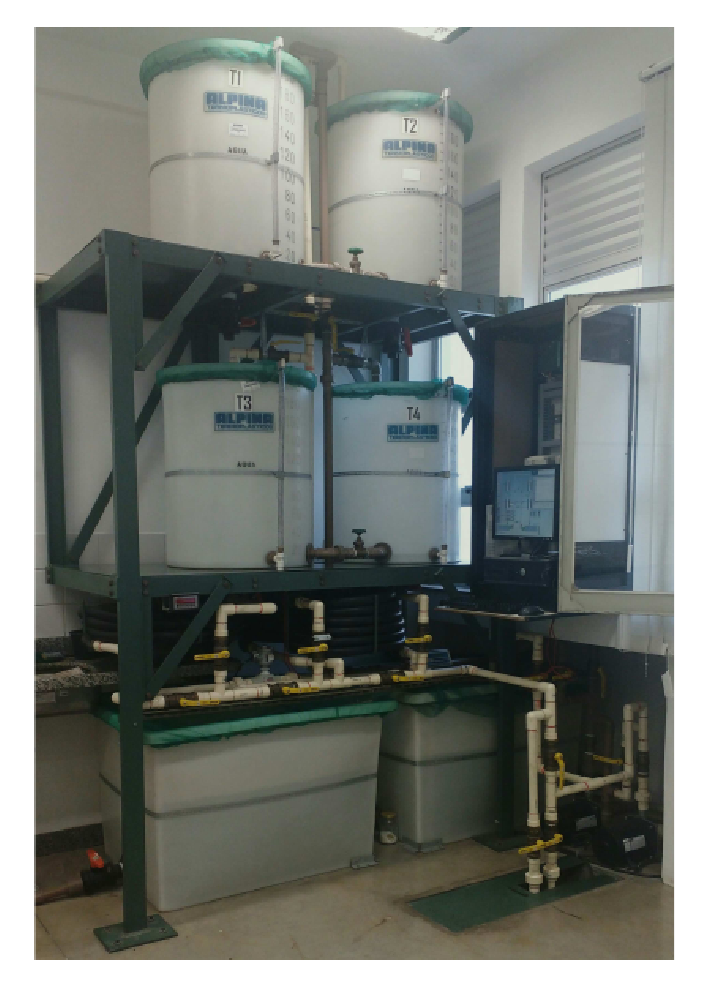
\includegraphics[height=.5\textheight]{imgs/tanks-real}
  \caption[System of coupled tanks.]{System of coupled tanks with four 200L
    tanks. There are two pumps that can be configured through the pipes to fill
    any of the tanks. Tank T3 has a rigid body with a non-linear shape inside
    it. The water flow between tanks is also configurable.}%
  \label{fig:tanks-real}
\end{figure}

\begin{figure}[ht!]
  \centering
  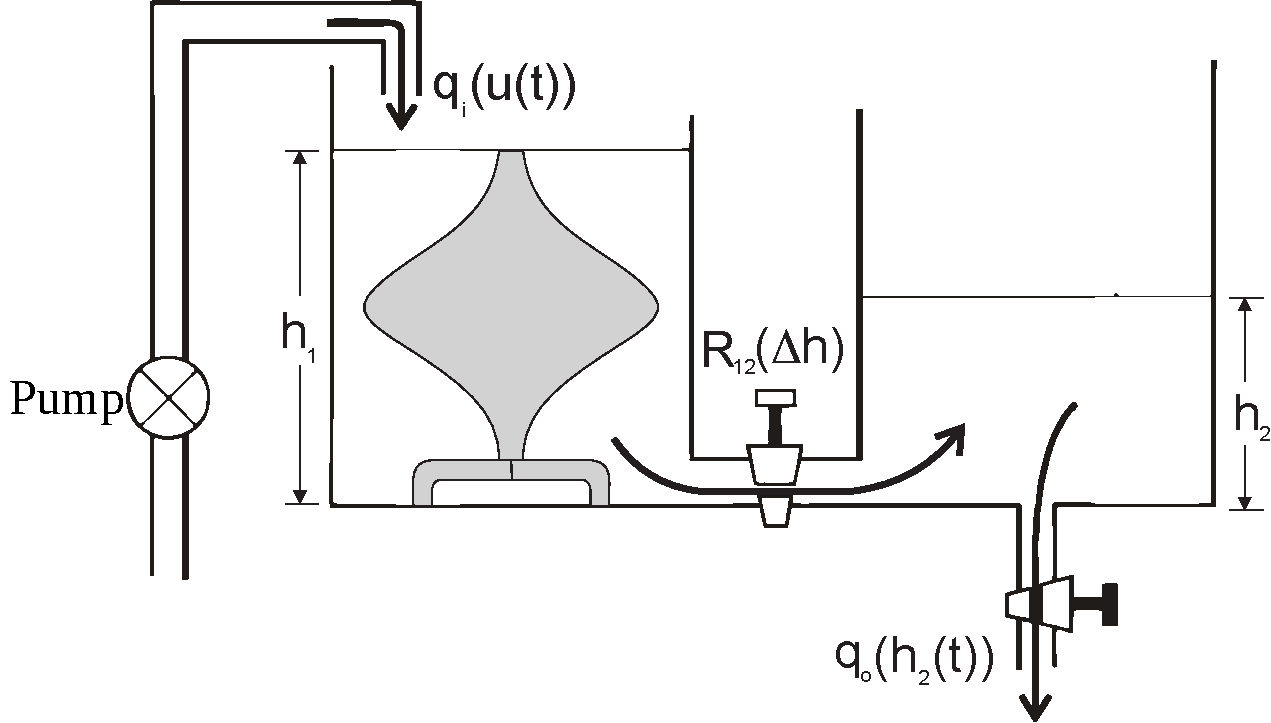
\includegraphics[width=0.9\linewidth]{imgs/tanks}
  \caption[Coupled tanks diagram.]{Diagram of the third and fourth tanks,
    showing the non-linear body. The water flows from the pump into the tank
    three, then move to tank four and goes back to the reservoir.}%
  \label{fig:tanks}
\end{figure}

Both tanks have the same cross-section area, denoted as \(A\)
(\si{\square\centi\metre}), however, there is a solid inside \(T1\) that makes its
area non-linear and adds uncertainties to its model. The cross-section area of
\(T1\) becomes
%
\begin{equation}
  \label{eq:t1-area}
  A_{1}(h_{1}(t)) = \frac{3r}{5} \left(
  2.7r - \frac{\cos(2.5\pi{}((h_{1}(t)-8)\times{}10^{-2}-\mu))}{\sigma{}\sqrt{2\pi}}
  e^{-\frac{((h_{1}(t)-8)\times{}10^{-2}-\mu^{2})^{2}}{2\sigma^{2}}}
  \right),
\end{equation}
%
where \(\mu=0.4\), \(\sigma=0.55\) and \(r=0.31\). The cross-section area of \(T2\) is
\(\SI{0.31}{\square\metre}\).

By using Bernoulli's equations, the system's dynamics can be described by:
%
\begin{equation}
  \label{eq:formula-height-variation}
  \begin{aligned}
    \dot{h}_1(t) & = \frac{R_{12}(h_{1}(t),h_{2}(t))\times{}K_{b}\times{}u(t)-h_{1}(t)+h_{2}(t)}
    {A_{1}(h_{1}(t))\times{}R_{12}(h_{1}(t),h_{2}(t))}                                                                 \\
    \dot{h}_2(t) & = \frac{h_{1}(t)-h_{2}(t)}{R_{12}(h_{1}(t),h_{2}(t))\times{}A_{2}} - \frac{q_{o}(h_{2}(t))}{A_{2}},
  \end{aligned}
\end{equation}
%
where \(R_{12}(h_{1}(t),h_{2}(t))=(0.412(h_{1}(t-h_{2}(t))+11.488)\times{}10^{-3}\)
and \(q_{o}(h_{2}(t))=11.941h_{2}(t)+787.586\). A frequency inverter controls
the pump through the percentage of maximum flow, and this value can be converted
to flow by \(q_{i}=13.201u_{t}+220.085\). Applying this before inputing in
Equation~\eqref{eq:formula-height-variation} results in \(u(t)\) becoming this
percentual value instead of the flow directly.

We chose four operation points to cover a significant portion of the available
\(h_{1}\) range (0 to \SI{70}{\centi\metre}), which is the output of the system.
The points and their respective linearized and discretized (with a sampling time
of \SI{5}{\second}) systems are

\begin{align*}
  \label{eq:op-points}
  \left[\begin{array}{c|c}
      x_{eq}^{\top} & u_{eq} \\
      \hline
      A             & B
    \end{array}\right]_{1} & = \left[\begin{array}{cc|c}
      19.5  & 5    & 15     \\
      \hline
      0.91  & 0.14 & 0.028  \\
      0.085 & 0.9  & 0.0013
    \end{array}\right],
  \left[\begin{array}{c|c}
      x_{eq}^{\top} & u_{eq} \\
      \hline
      A             & B
    \end{array}\right]_{2} & = \left[\begin{array}{cc|c}
      27.5  & 11.6 & 20     \\
      \hline
      0.94  & 0.19 & 0.04   \\
      0.084 & 0.9  & 0.0018
    \end{array}\right], \\
  \left[\begin{array}{c|c}
      x_{eq}^{\top} & u_{eq} \\
      \hline
      A             & B
    \end{array}\right]_{3} & = \left[\begin{array}{cc|c}
      37.3  & 17.8 & 25     \\
      \hline
      1.1   & 0.47 & 0.1    \\
      0.086 & 0.92 & 0.0042
    \end{array}\right],
  \left[\begin{array}{c|c}
      x_{eq}^{\top} & u_{eq} \\
      \hline
      A             & B
    \end{array}\right]_{4} & = \left[\begin{array}{cc|c}
      47.4  & 24.9 & 30     \\
      \hline
      0.49  & 0.96 & 0.22   \\
      0.053 & 0.95 & 0.0096
    \end{array}\right].
\end{align*}

To develop the controllers we applied the LMI described in the
Section~\ref{sec:region-of-attraction}~-~\nameref{sec:region-of-attraction} to
the integral-augmented system. The augmented state is the integral of the
output, \(h_{1}\). The points forced to be inside the region of attraction are
the previous' and next's operation point. It creates an intersection that allows
the early switching of controllers, which speeds up convergence. The following
controllers were obtained:

\begin{align}
  K_{1} & = \begin{bmatrix} -12.884 & -97.540 & -13.975 \end{bmatrix}, \\
  K_{2} & = \begin{bmatrix} -10.054 & -73.777 & -10.523 \end{bmatrix}, \\
  K_{3} & = \begin{bmatrix} -5.840  & -31.622 & -4.148 \end{bmatrix}, \\
  K_{4} & = \begin{bmatrix} -1.832  & -21.527 & -4.177 \end{bmatrix}.
\end{align}

To calculate each of the described modes' dwell-time, we applied the technique
described by~\textcite{franzè.lucia.ea:command}. We then ran both approaches ---
the dwell-time and the proposed one --- on the physical system.
Figures~\ref{fig:tanks-dwell} and~\ref{fig:tanks-roa} show the result of the
experiments, where the colored backgrounds represent the different modes, M1 to
M4, the two states (\(x_{1}\) and \(x_{2}\)) are plotted alongside their
respective real (\(r_{1,2}\)) and virtual (\(g_{1,2}\)) references.

The proposed technique has a faster overall convergence, entering the final mode
after 215 seconds while the dwell-time approach takes 340 seconds. This can
easily be seen by comparing the width of the regions with different background
colors, as the red, orange and yellow regions are much shorter on the proposed
technique. The proposed approach also shows no overshoot, since it does not give
the system enough time to converge to the waypoints and keeps it always moving
towards the reference, as shown by the states' trajectories, which are always
moving torwards the reference in the proposed technique, but starts to converge
to the mode's operation point on the dwell-time technique. Because of that, it
also has a smaller control effort, producing smaller control signal variation,
seen in the last plot, where the control signal constantly saturates in the
dwell-time approach, but does not saturate and has a smaller variation in the
proposed technique.

The last mode should also have an overshoot on the proposed technique, since it
is part of the closed-loop dynamics. However, the command governor's
optimization problem generated virtual references that slowly guided the system
to the real reference, making it take longer than necessary to converge. The
behaviour was present on every test repetition, just like the dwell-time
approach's overshoots.

\begin{figure}[ht!]
  \centering
  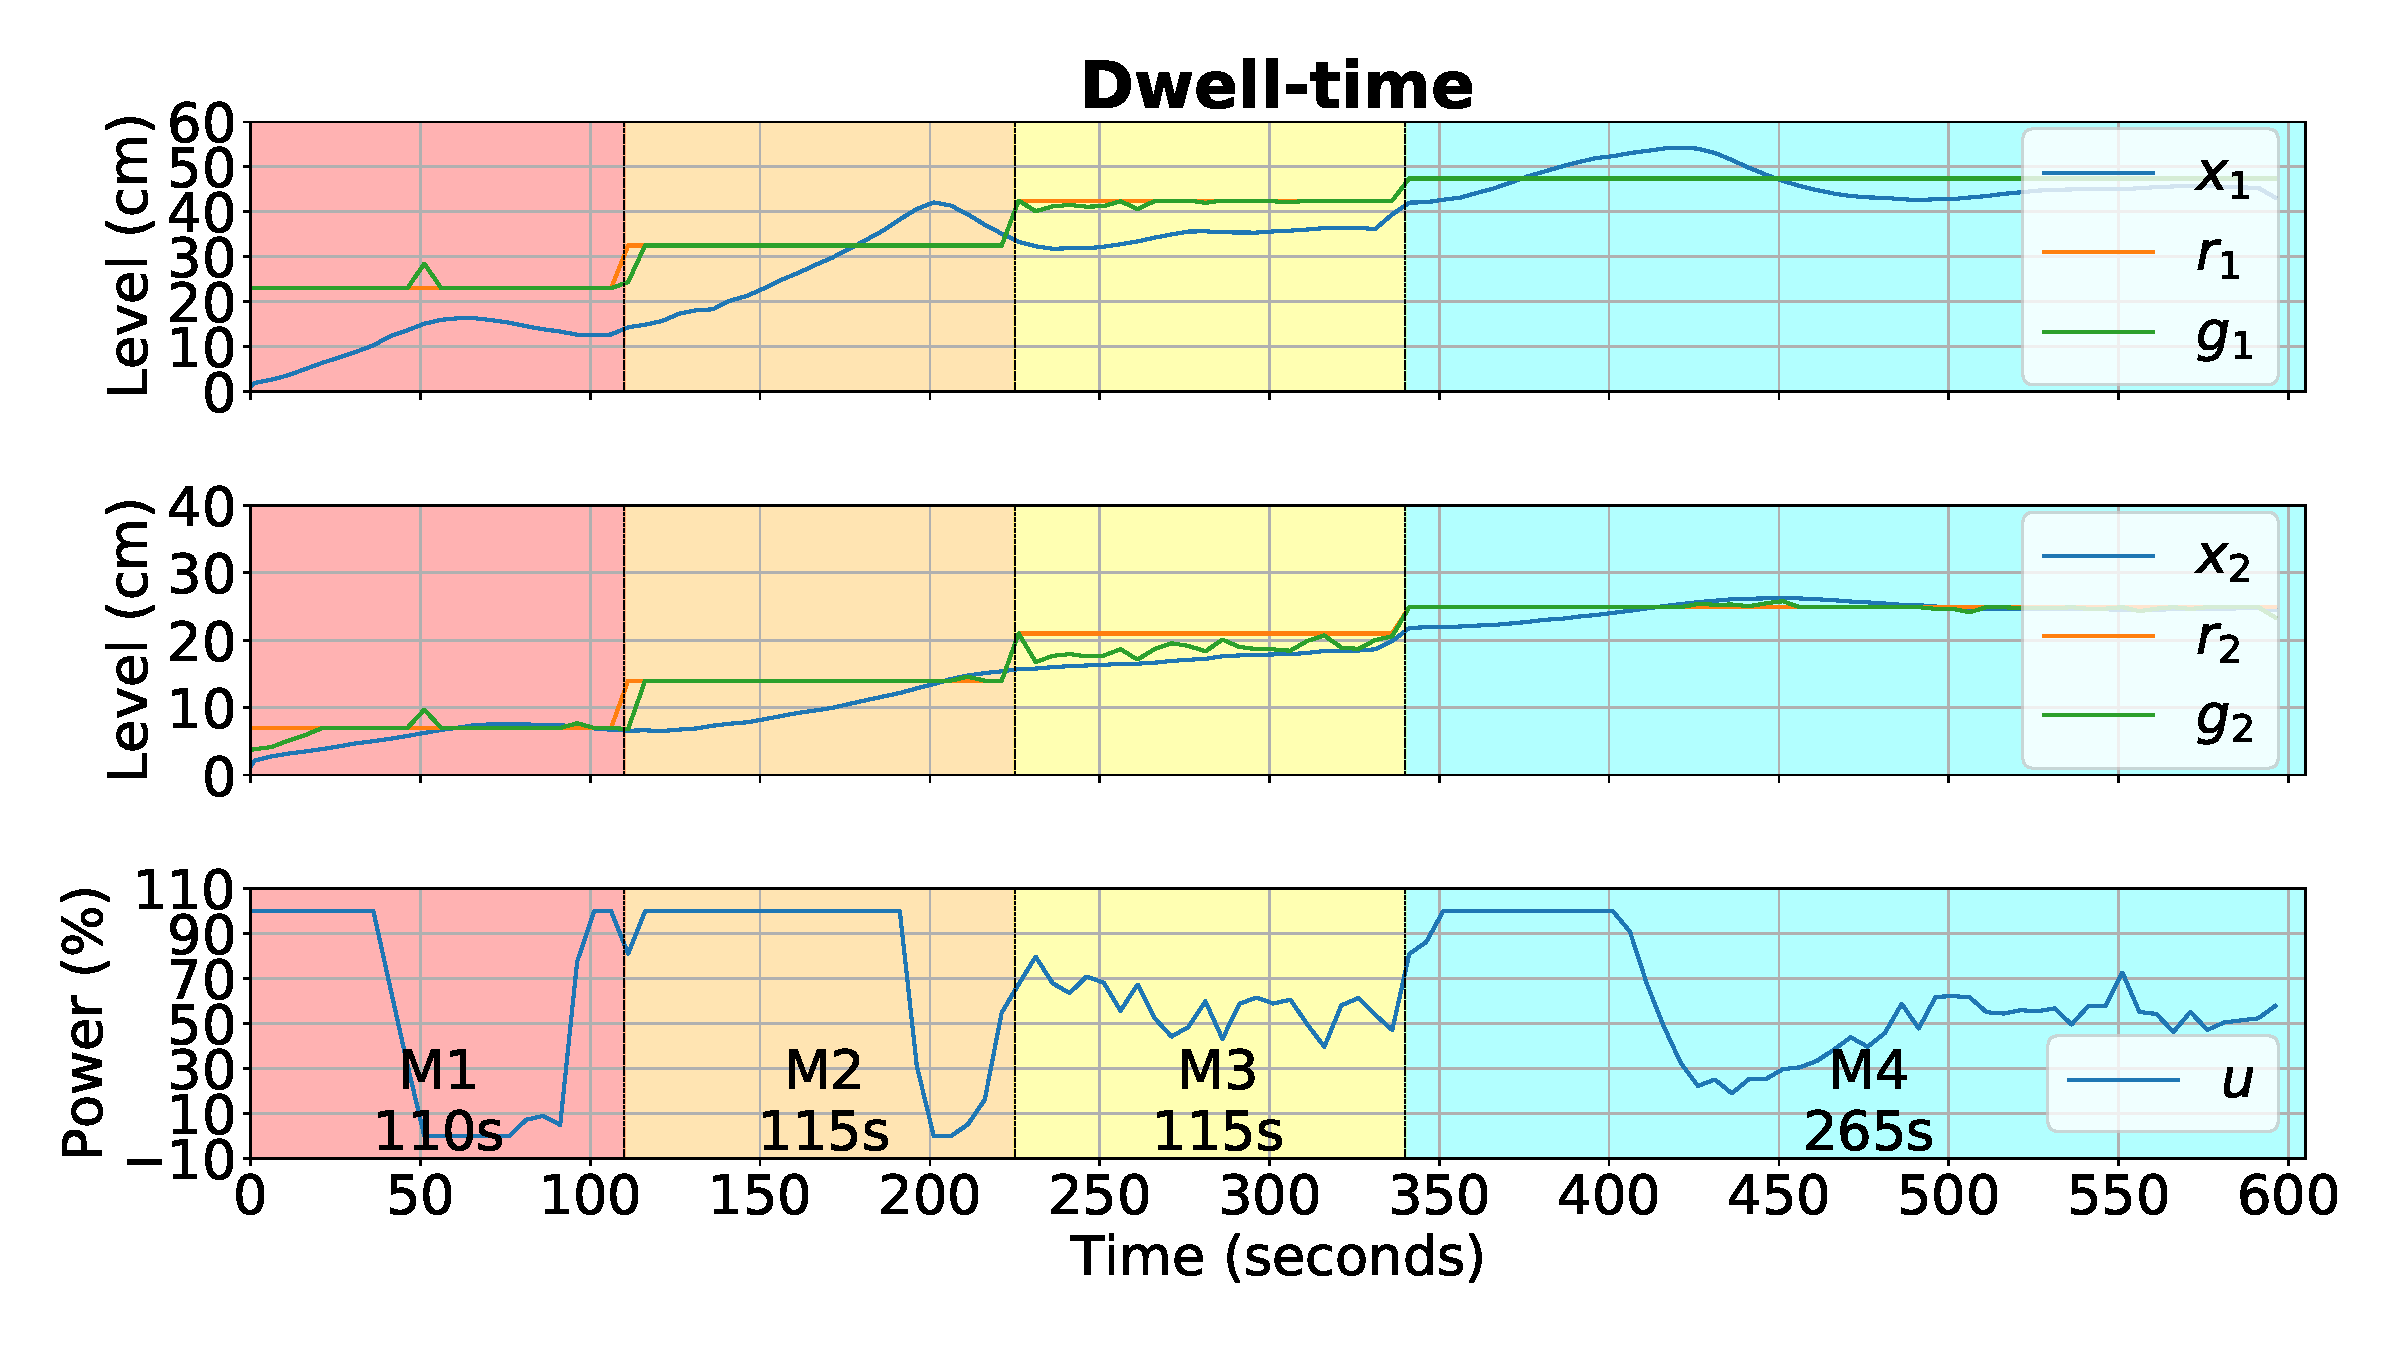
\includegraphics[width=\linewidth]{imgs/tanks-dwell}
  \caption[Experimental dwell-time states.]{This Figure shows the states and
    control signal of the system running with the dwell-time rule. The first two
    plots show the system states as well as the reference set by the supervisor
    and command governors and the third plot shows the control signal. All plots
    have colored backgrounds displaying the active mode, and the last plot also
    shows the time that each mode remained active. The states show overflows on
    first, second and fourth modes, which is expected from the system, and the
    control signal saturates four times and presents a large variation, going
    from 100\% to 0\%.}%
  \label{fig:tanks-dwell}
\end{figure}

\begin{figure}[ht!]
  \centering
  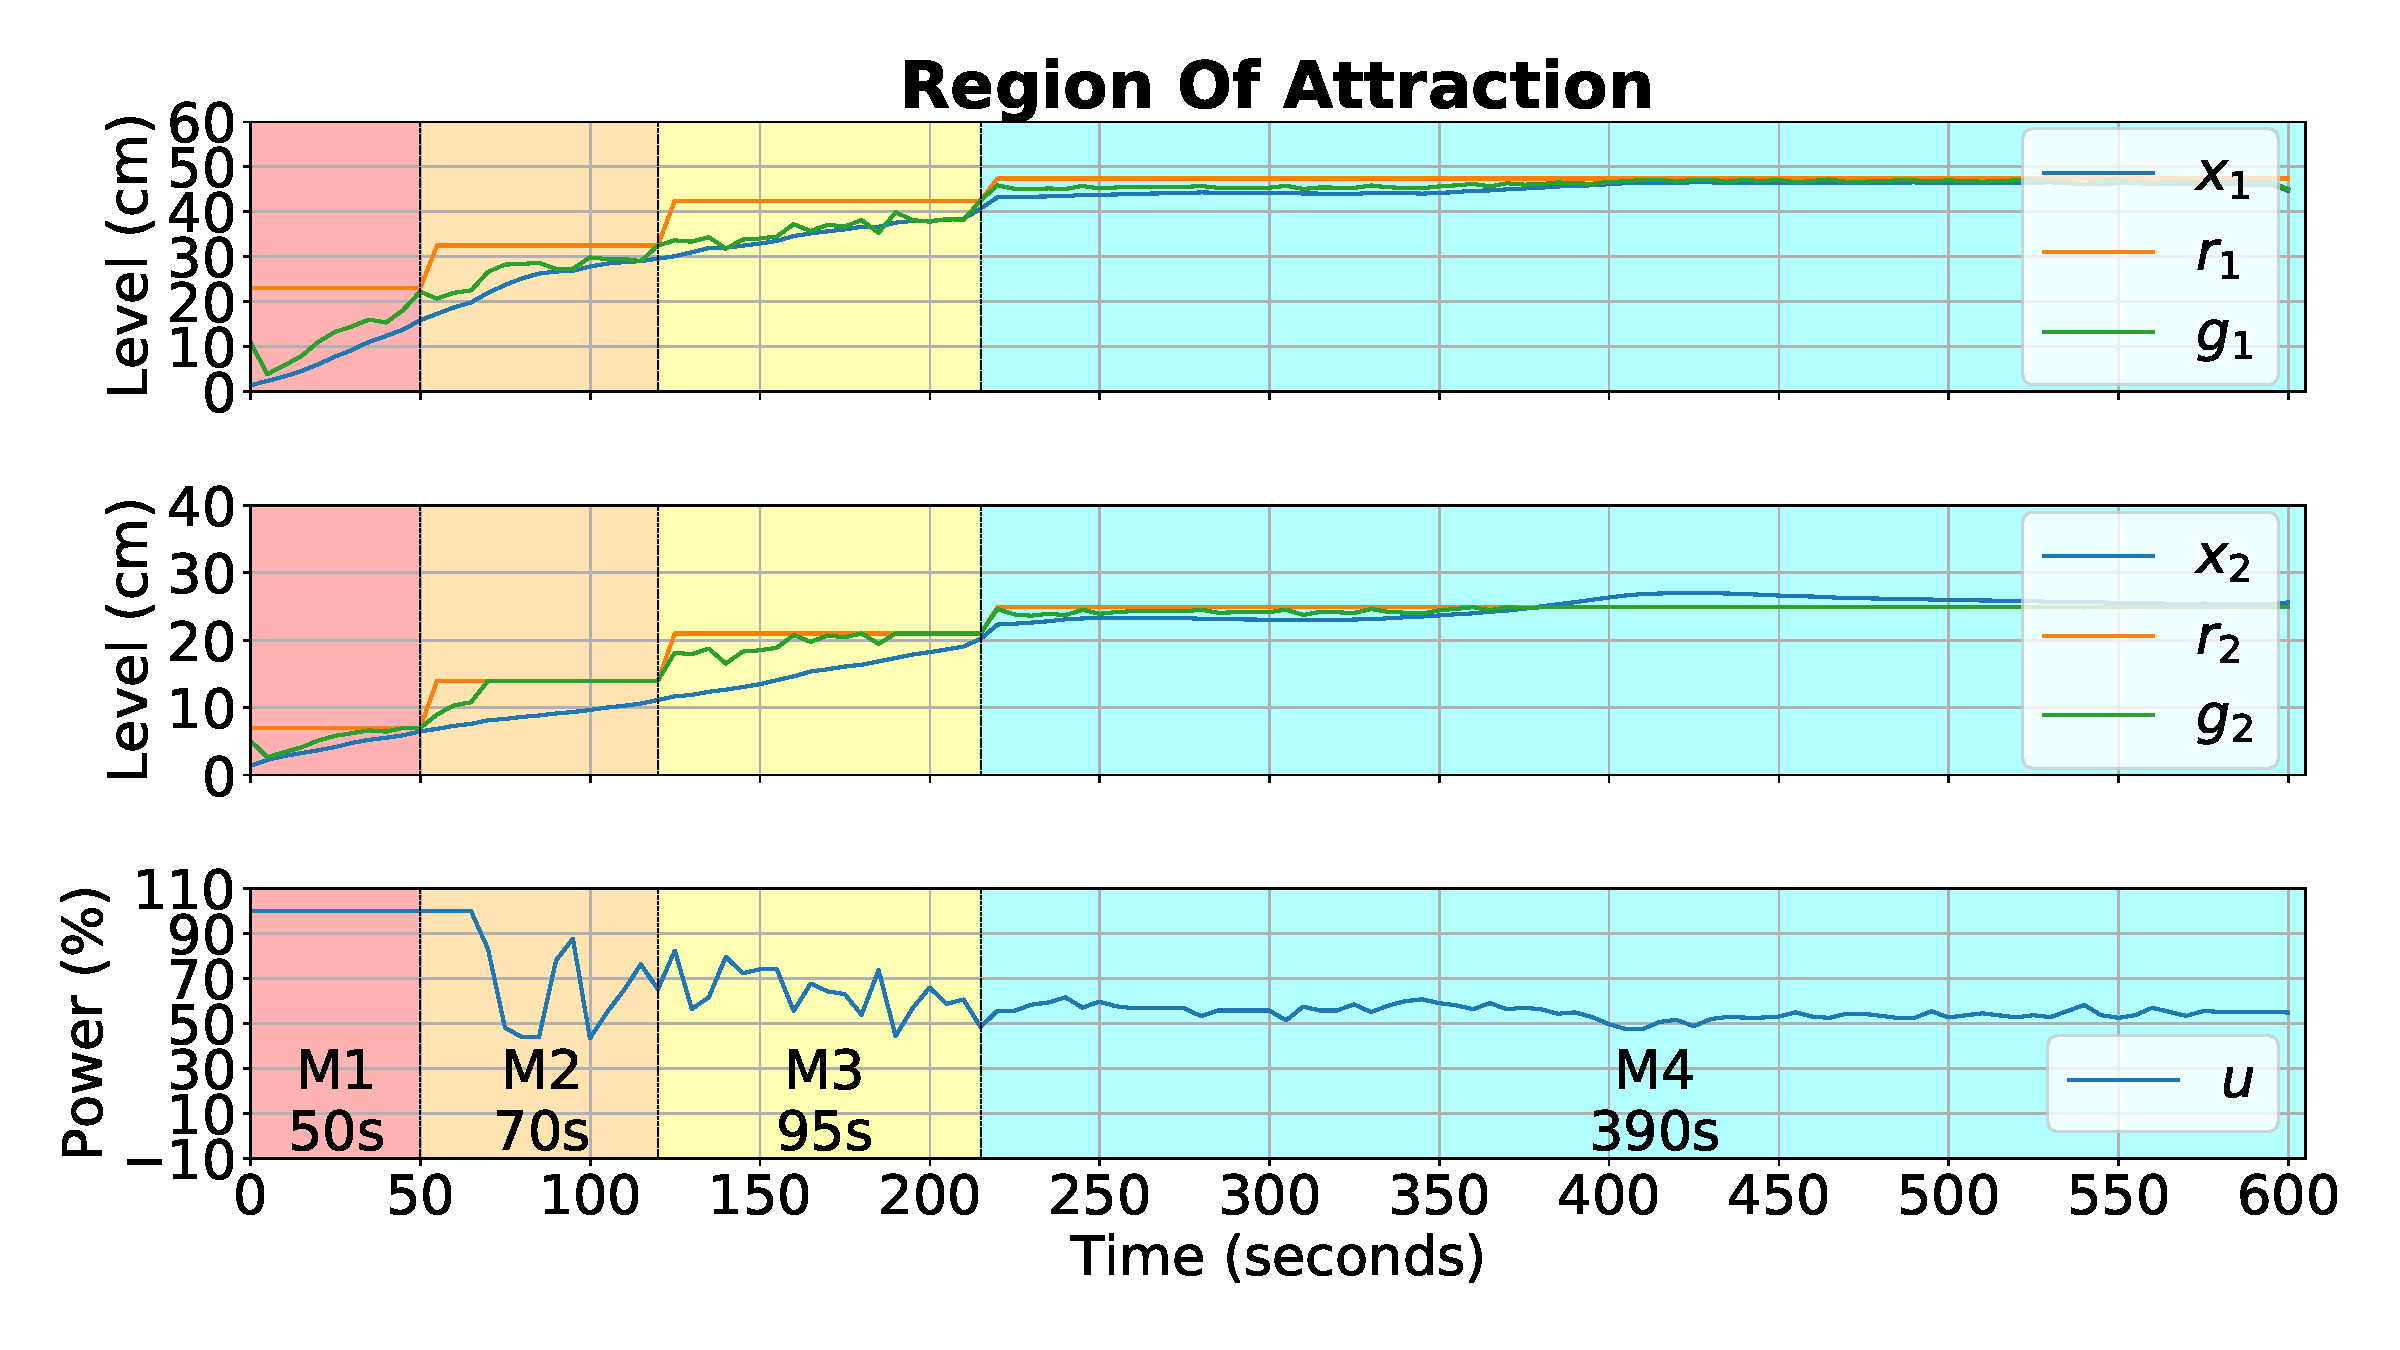
\includegraphics[width=\linewidth]{imgs/tanks-roa}
  \caption[Experimental RoA states.]{This Figure show the states and control
    signals of the Region of Attraction-based switching rule. It has the same
    structure as Figure~\ref{fig:tanks-dwell}. The overall convergence is
    visibly faster than the dwell-time alternative. Also, the states do not
    present overshoots, since the system is not given enough time to converge to
    the waypoints. The control signal has a smaler variation in amplitude only
    saturates at the begining.}%
  \label{fig:tanks-roa}
\end{figure}

% !TeX root = document.tex
% !TeX encoding = UTF-8 Unicode

\chapter{Final Considerations}%
\label{chp:final-considerations}

Final Considerations

\printbibliography{}
\end{document}
